\documentclass[twoside]{book}

% Packages required by doxygen
\usepackage{fixltx2e}
\usepackage{calc}
\usepackage{doxygen}
\usepackage[export]{adjustbox} % also loads graphicx
\usepackage{graphicx}
\usepackage[utf8]{inputenc}
\usepackage{makeidx}
\usepackage{multicol}
\usepackage{multirow}
\PassOptionsToPackage{warn}{textcomp}
\usepackage{textcomp}
\usepackage[nointegrals]{wasysym}
\usepackage[table]{xcolor}

% Font selection
\usepackage[T1]{fontenc}
\usepackage[scaled=.90]{helvet}
\usepackage{courier}
\usepackage{amssymb}
\usepackage{sectsty}
\renewcommand{\familydefault}{\sfdefault}
\allsectionsfont{%
  \fontseries{bc}\selectfont%
  \color{darkgray}%
}
\renewcommand{\DoxyLabelFont}{%
  \fontseries{bc}\selectfont%
  \color{darkgray}%
}
\newcommand{\+}{\discretionary{\mbox{\scriptsize$\hookleftarrow$}}{}{}}

% Page & text layout
\usepackage{geometry}
\geometry{%
  a4paper,%
  top=2.5cm,%
  bottom=2.5cm,%
  left=2.5cm,%
  right=2.5cm%
}
\tolerance=750
\hfuzz=15pt
\hbadness=750
\setlength{\emergencystretch}{15pt}
\setlength{\parindent}{0cm}
\setlength{\parskip}{3ex plus 2ex minus 2ex}
\makeatletter
\renewcommand{\paragraph}{%
  \@startsection{paragraph}{4}{0ex}{-1.0ex}{1.0ex}{%
    \normalfont\normalsize\bfseries\SS@parafont%
  }%
}
\renewcommand{\subparagraph}{%
  \@startsection{subparagraph}{5}{0ex}{-1.0ex}{1.0ex}{%
    \normalfont\normalsize\bfseries\SS@subparafont%
  }%
}
\makeatother

% Headers & footers
\usepackage{fancyhdr}
\pagestyle{fancyplain}
\fancyhead[LE]{\fancyplain{}{\bfseries\thepage}}
\fancyhead[CE]{\fancyplain{}{}}
\fancyhead[RE]{\fancyplain{}{\bfseries\leftmark}}
\fancyhead[LO]{\fancyplain{}{\bfseries\rightmark}}
\fancyhead[CO]{\fancyplain{}{}}
\fancyhead[RO]{\fancyplain{}{\bfseries\thepage}}
\fancyfoot[LE]{\fancyplain{}{}}
\fancyfoot[CE]{\fancyplain{}{}}
\fancyfoot[RE]{\fancyplain{}{\bfseries\scriptsize Generated by Doxygen }}
\fancyfoot[LO]{\fancyplain{}{\bfseries\scriptsize Generated by Doxygen }}
\fancyfoot[CO]{\fancyplain{}{}}
\fancyfoot[RO]{\fancyplain{}{}}
\renewcommand{\footrulewidth}{0.4pt}
\renewcommand{\chaptermark}[1]{%
  \markboth{#1}{}%
}
\renewcommand{\sectionmark}[1]{%
  \markright{\thesection\ #1}%
}

% Indices & bibliography
\usepackage{natbib}
\usepackage[titles]{tocloft}
\setcounter{tocdepth}{3}
\setcounter{secnumdepth}{5}
\makeindex

% Hyperlinks (required, but should be loaded last)
\usepackage{ifpdf}
\ifpdf
  \usepackage[pdftex,pagebackref=true]{hyperref}
\else
  \usepackage[ps2pdf,pagebackref=true]{hyperref}
\fi
\hypersetup{%
  colorlinks=true,%
  linkcolor=blue,%
  citecolor=blue,%
  unicode%
}

% Custom commands
\newcommand{\clearemptydoublepage}{%
  \newpage{\pagestyle{empty}\cleardoublepage}%
}

\usepackage{caption}
\captionsetup{labelsep=space,justification=centering,font={bf},singlelinecheck=off,skip=4pt,position=top}

%===== C O N T E N T S =====

\begin{document}

% Titlepage & ToC
\hypersetup{pageanchor=false,
             bookmarksnumbered=true,
             pdfencoding=unicode
            }
\pagenumbering{alph}
\begin{titlepage}
\vspace*{7cm}
\begin{center}%
{\Large Dice }\\
\vspace*{1cm}
{\large Generated by Doxygen 1.8.14}\\
\end{center}
\end{titlepage}
\clearemptydoublepage
\pagenumbering{roman}
\tableofcontents
\clearemptydoublepage
\pagenumbering{arabic}
\hypersetup{pageanchor=true}

%--- Begin generated contents ---
\chapter{Hierarchical Index}
\section{Class Hierarchy}
This inheritance list is sorted roughly, but not completely, alphabetically\+:\begin{DoxyCompactList}
\item \contentsline{section}{dice\+:\+:base\+\_\+value}{\pageref{classdice_1_1base__value}}{}
\begin{DoxyCompactList}
\item \contentsline{section}{dice\+:\+:typed\+\_\+value$<$ T $>$}{\pageref{classdice_1_1typed__value}}{}
\end{DoxyCompactList}
\item \contentsline{section}{dice\+:\+:bernoulli\+\_\+tag}{\pageref{classdice_1_1bernoulli__tag}}{}
\item \contentsline{section}{dice\+:\+:calculator}{\pageref{structdice_1_1calculator}}{}
\item \contentsline{section}{command\+\_\+reader}{\pageref{structcommand__reader}}{}
\item \contentsline{section}{dice\+:\+:constant\+\_\+tag}{\pageref{classdice_1_1constant__tag}}{}
\item \contentsline{section}{dice\+:\+:conversions}{\pageref{classdice_1_1conversions}}{}
\item \contentsline{section}{dice\+:\+:decomposition$<$ Value\+Type, Probability\+Type $>$}{\pageref{classdice_1_1decomposition}}{}
\item \contentsline{section}{dice\+:\+:decomposition\+\_\+iterator$<$ Value\+Type, Probability\+Type $>$}{\pageref{classdice_1_1decomposition__iterator}}{}
\item \contentsline{section}{dice\+:\+:direct\+\_\+interpreter$<$ Environment $>$}{\pageref{classdice_1_1direct__interpreter}}{}
\item \contentsline{section}{dice\+:\+:direct\+\_\+interpreter$<$ dice\+:\+:environment $>$}{\pageref{classdice_1_1direct__interpreter}}{}
\item \contentsline{section}{dice\+:\+:environment}{\pageref{classdice_1_1environment}}{}
\item \contentsline{section}{dice\+:\+:execution\+\_\+context}{\pageref{classdice_1_1execution__context}}{}
\item \contentsline{section}{dice\+:\+:function\+\_\+definition}{\pageref{classdice_1_1function__definition}}{}
\item \contentsline{section}{std\+:\+:hash$<$ dice\+:\+:safe$<$ T $>$ $>$}{\pageref{structstd_1_1hash_3_01dice_1_1safe_3_01T_01_4_01_4}}{}
\item \contentsline{section}{dice\+:\+:lexer$<$ Logger $>$}{\pageref{classdice_1_1lexer}}{}
\item \contentsline{section}{dice\+:\+:lexer\+\_\+location}{\pageref{structdice_1_1lexer__location}}{}
\item \contentsline{section}{dice\+:\+:logger}{\pageref{classdice_1_1logger}}{}
\item logic\+\_\+error\begin{DoxyCompactList}
\item \contentsline{section}{dice\+:\+:compiler\+\_\+error}{\pageref{classdice_1_1compiler__error}}{}
\end{DoxyCompactList}
\item \contentsline{section}{dice\+:\+:nonterminal$<$ type $>$}{\pageref{classdice_1_1nonterminal}}{}
\item \contentsline{section}{dice\+:\+:nonterminal$<$ nonterminal\+\_\+type\+:\+:add $>$}{\pageref{classdice_1_1nonterminal_3_01nonterminal__type_1_1add_01_4}}{}
\item \contentsline{section}{dice\+:\+:nonterminal$<$ nonterminal\+\_\+type\+:\+:dice\+\_\+roll $>$}{\pageref{classdice_1_1nonterminal_3_01nonterminal__type_1_1dice__roll_01_4}}{}
\item \contentsline{section}{dice\+:\+:nonterminal$<$ nonterminal\+\_\+type\+:\+:expr $>$}{\pageref{classdice_1_1nonterminal_3_01nonterminal__type_1_1expr_01_4}}{}
\item \contentsline{section}{dice\+:\+:nonterminal$<$ nonterminal\+\_\+type\+:\+:factor $>$}{\pageref{classdice_1_1nonterminal_3_01nonterminal__type_1_1factor_01_4}}{}
\item \contentsline{section}{dice\+:\+:nonterminal$<$ nonterminal\+\_\+type\+:\+:mult $>$}{\pageref{classdice_1_1nonterminal_3_01nonterminal__type_1_1mult_01_4}}{}
\item \contentsline{section}{dice\+:\+:nonterminal$<$ nonterminal\+\_\+type\+:\+:param\+\_\+list $>$}{\pageref{classdice_1_1nonterminal_3_01nonterminal__type_1_1param__list_01_4}}{}
\item \contentsline{section}{dice\+:\+:nonterminal$<$ nonterminal\+\_\+type\+:\+:stmt $>$}{\pageref{classdice_1_1nonterminal_3_01nonterminal__type_1_1stmt_01_4}}{}
\item \contentsline{section}{dice\+:\+:nonterminal$<$ nonterminal\+\_\+type\+:\+:stmts $>$}{\pageref{classdice_1_1nonterminal_3_01nonterminal__type_1_1stmts_01_4}}{}
\item \contentsline{section}{std\+:\+:numeric\+\_\+limits$<$ dice\+:\+:safe$<$ T $>$ $>$}{\pageref{classstd_1_1numeric__limits_3_01dice_1_1safe_3_01T_01_4_01_4}}{}
\item \contentsline{section}{options}{\pageref{structoptions}}{}
\item \contentsline{section}{dice\+:\+:parser$<$ Lexer, Logger, Interpreter $>$}{\pageref{classdice_1_1parser}}{}
\item \contentsline{section}{dice\+:\+:random\+\_\+variable$<$ Value\+Type, Probability\+Type $>$}{\pageref{classdice_1_1random__variable}}{}
\item \contentsline{section}{dice\+:\+:symbol}{\pageref{structdice_1_1symbol}}{}
\item \contentsline{section}{dice\+:\+:value\+\_\+visitor}{\pageref{classdice_1_1value__visitor}}{}
\begin{DoxyCompactList}
\item \contentsline{section}{dice\+:\+:conversion\+\_\+visitor}{\pageref{classdice_1_1conversion__visitor}}{}
\item \contentsline{section}{formatting\+\_\+visitor}{\pageref{classformatting__visitor}}{}
\end{DoxyCompactList}
\end{DoxyCompactList}

\chapter{Class Index}
\section{Class List}
Here are the classes, structs, unions and interfaces with brief descriptions\+:\begin{DoxyCompactList}
\item\contentsline{section}{\mbox{\hyperlink{classdice_1_1base__value}{dice\+::base\+\_\+value}} \\*Parent of all value types that are used in dice expressions }{\pageref{classdice_1_1base__value}}{}
\item\contentsline{section}{\mbox{\hyperlink{classdice_1_1bernoulli__tag}{dice\+::bernoulli\+\_\+tag}} }{\pageref{classdice_1_1bernoulli__tag}}{}
\item\contentsline{section}{\mbox{\hyperlink{structdice_1_1calculator}{dice\+::calculator}} \\*Facade for script evaluation }{\pageref{structdice_1_1calculator}}{}
\item\contentsline{section}{\mbox{\hyperlink{structcommand__reader}{command\+\_\+reader}} }{\pageref{structcommand__reader}}{}
\item\contentsline{section}{\mbox{\hyperlink{classdice_1_1compiler__error}{dice\+::compiler\+\_\+error}} \\*An error thrown when there is an error in computation during script evaluation }{\pageref{classdice_1_1compiler__error}}{}
\item\contentsline{section}{\mbox{\hyperlink{classdice_1_1constant__tag}{dice\+::constant\+\_\+tag}} }{\pageref{classdice_1_1constant__tag}}{}
\item\contentsline{section}{\mbox{\hyperlink{classdice_1_1conversion__visitor}{dice\+::conversion\+\_\+visitor}} }{\pageref{classdice_1_1conversion__visitor}}{}
\item\contentsline{section}{\mbox{\hyperlink{classdice_1_1conversions}{dice\+::conversions}} \\*This class manages conversions of values in dice expression }{\pageref{classdice_1_1conversions}}{}
\item\contentsline{section}{\mbox{\hyperlink{classdice_1_1decomposition}{dice\+::decomposition$<$ Value\+Type, Probability\+Type $>$}} \\*Object representing a decomposition of a function of random variables }{\pageref{classdice_1_1decomposition}}{}
\item\contentsline{section}{\mbox{\hyperlink{classdice_1_1decomposition__iterator}{dice\+::decomposition\+\_\+iterator$<$ Value\+Type, Probability\+Type $>$}} \\*Decompositon value iterator }{\pageref{classdice_1_1decomposition__iterator}}{}
\item\contentsline{section}{\mbox{\hyperlink{classdice_1_1direct__interpreter}{dice\+::direct\+\_\+interpreter$<$ Environment $>$}} \\*This interpreter evaluates expressions as soon as they are parsed }{\pageref{classdice_1_1direct__interpreter}}{}
\item\contentsline{section}{\mbox{\hyperlink{classdice_1_1environment}{dice\+::environment}} \\*Symbol table }{\pageref{classdice_1_1environment}}{}
\item\contentsline{section}{\mbox{\hyperlink{classdice_1_1execution__context}{dice\+::execution\+\_\+context}} \\*Context of dice user function execution }{\pageref{classdice_1_1execution__context}}{}
\item\contentsline{section}{\mbox{\hyperlink{classformatting__visitor}{formatting\+\_\+visitor}} }{\pageref{classformatting__visitor}}{}
\item\contentsline{section}{\mbox{\hyperlink{classdice_1_1function__definition}{dice\+::function\+\_\+definition}} \\*Object representing a function callable from a dice expression }{\pageref{classdice_1_1function__definition}}{}
\item\contentsline{section}{\mbox{\hyperlink{structstd_1_1hash_3_01dice_1_1safe_3_01T_01_4_01_4}{std\+::hash$<$ dice\+::safe$<$ T $>$ $>$}} }{\pageref{structstd_1_1hash_3_01dice_1_1safe_3_01T_01_4_01_4}}{}
\item\contentsline{section}{\mbox{\hyperlink{classdice_1_1lexer}{dice\+::lexer$<$ Logger $>$}} \\*Lexer of a dice script }{\pageref{classdice_1_1lexer}}{}
\item\contentsline{section}{\mbox{\hyperlink{structdice_1_1lexer__location}{dice\+::lexer\+\_\+location}} \\*Location in an input stream }{\pageref{structdice_1_1lexer__location}}{}
\item\contentsline{section}{\mbox{\hyperlink{classdice_1_1logger}{dice\+::logger}} \\*This class prints all errors in given output stream }{\pageref{classdice_1_1logger}}{}
\item\contentsline{section}{\mbox{\hyperlink{classdice_1_1nonterminal}{dice\+::nonterminal$<$ type $>$}} }{\pageref{classdice_1_1nonterminal}}{}
\item\contentsline{section}{\mbox{\hyperlink{classdice_1_1nonterminal_3_01nonterminal__type_1_1add_01_4}{dice\+::nonterminal$<$ nonterminal\+\_\+type\+::add $>$}} }{\pageref{classdice_1_1nonterminal_3_01nonterminal__type_1_1add_01_4}}{}
\item\contentsline{section}{\mbox{\hyperlink{classdice_1_1nonterminal_3_01nonterminal__type_1_1dice__roll_01_4}{dice\+::nonterminal$<$ nonterminal\+\_\+type\+::dice\+\_\+roll $>$}} }{\pageref{classdice_1_1nonterminal_3_01nonterminal__type_1_1dice__roll_01_4}}{}
\item\contentsline{section}{\mbox{\hyperlink{classdice_1_1nonterminal_3_01nonterminal__type_1_1expr_01_4}{dice\+::nonterminal$<$ nonterminal\+\_\+type\+::expr $>$}} }{\pageref{classdice_1_1nonterminal_3_01nonterminal__type_1_1expr_01_4}}{}
\item\contentsline{section}{\mbox{\hyperlink{classdice_1_1nonterminal_3_01nonterminal__type_1_1factor_01_4}{dice\+::nonterminal$<$ nonterminal\+\_\+type\+::factor $>$}} }{\pageref{classdice_1_1nonterminal_3_01nonterminal__type_1_1factor_01_4}}{}
\item\contentsline{section}{\mbox{\hyperlink{classdice_1_1nonterminal_3_01nonterminal__type_1_1mult_01_4}{dice\+::nonterminal$<$ nonterminal\+\_\+type\+::mult $>$}} }{\pageref{classdice_1_1nonterminal_3_01nonterminal__type_1_1mult_01_4}}{}
\item\contentsline{section}{\mbox{\hyperlink{classdice_1_1nonterminal_3_01nonterminal__type_1_1param__list_01_4}{dice\+::nonterminal$<$ nonterminal\+\_\+type\+::param\+\_\+list $>$}} }{\pageref{classdice_1_1nonterminal_3_01nonterminal__type_1_1param__list_01_4}}{}
\item\contentsline{section}{\mbox{\hyperlink{classdice_1_1nonterminal_3_01nonterminal__type_1_1stmt_01_4}{dice\+::nonterminal$<$ nonterminal\+\_\+type\+::stmt $>$}} }{\pageref{classdice_1_1nonterminal_3_01nonterminal__type_1_1stmt_01_4}}{}
\item\contentsline{section}{\mbox{\hyperlink{classdice_1_1nonterminal_3_01nonterminal__type_1_1stmts_01_4}{dice\+::nonterminal$<$ nonterminal\+\_\+type\+::stmts $>$}} }{\pageref{classdice_1_1nonterminal_3_01nonterminal__type_1_1stmts_01_4}}{}
\item\contentsline{section}{\mbox{\hyperlink{classstd_1_1numeric__limits_3_01dice_1_1safe_3_01T_01_4_01_4}{std\+::numeric\+\_\+limits$<$ dice\+::safe$<$ T $>$ $>$}} }{\pageref{classstd_1_1numeric__limits_3_01dice_1_1safe_3_01T_01_4_01_4}}{}
\item\contentsline{section}{\mbox{\hyperlink{structoptions}{options}} }{\pageref{structoptions}}{}
\item\contentsline{section}{\mbox{\hyperlink{classdice_1_1parser}{dice\+::parser$<$ Lexer, Logger, Interpreter $>$}} \\*Dice expression parser }{\pageref{classdice_1_1parser}}{}
\item\contentsline{section}{\mbox{\hyperlink{classdice_1_1random__variable}{dice\+::random\+\_\+variable$<$ Value\+Type, Probability\+Type $>$}} \\*Discrete random variable }{\pageref{classdice_1_1random__variable}}{}
\item\contentsline{section}{\mbox{\hyperlink{structdice_1_1symbol}{dice\+::symbol}} \\*Terminal symbol returned by the lexer type }{\pageref{structdice_1_1symbol}}{}
\item\contentsline{section}{\mbox{\hyperlink{classdice_1_1typed__value}{dice\+::typed\+\_\+value$<$ T $>$}} \\*Value with data }{\pageref{classdice_1_1typed__value}}{}
\item\contentsline{section}{\mbox{\hyperlink{classdice_1_1value__visitor}{dice\+::value\+\_\+visitor}} \\*Visitor of a dice value }{\pageref{classdice_1_1value__visitor}}{}
\end{DoxyCompactList}

\chapter{File Index}
\section{File List}
Here is a list of all documented files with brief descriptions\+:\begin{DoxyCompactList}
\item\contentsline{section}{C\+:/projects/dice/src/{\bfseries calculator.\+hpp} }{\pageref{calculator_8hpp}}{}
\item\contentsline{section}{C\+:/projects/dice/src/{\bfseries conversions.\+hpp} }{\pageref{conversions_8hpp}}{}
\item\contentsline{section}{C\+:/projects/dice/src/{\bfseries decomposition.\+hpp} }{\pageref{decomposition_8hpp}}{}
\item\contentsline{section}{C\+:/projects/dice/src/{\bfseries direct\+\_\+interpreter.\+hpp} }{\pageref{direct__interpreter_8hpp}}{}
\item\contentsline{section}{C\+:/projects/dice/src/{\bfseries environment.\+hpp} }{\pageref{environment_8hpp}}{}
\item\contentsline{section}{C\+:/projects/dice/src/{\bfseries functions.\+hpp} }{\pageref{functions_8hpp}}{}
\item\contentsline{section}{C\+:/projects/dice/src/{\bfseries lexer.\+hpp} }{\pageref{lexer_8hpp}}{}
\item\contentsline{section}{C\+:/projects/dice/src/{\bfseries logger.\+hpp} }{\pageref{logger_8hpp}}{}
\item\contentsline{section}{C\+:/projects/dice/src/{\bfseries parser.\+hpp} }{\pageref{parser_8hpp}}{}
\item\contentsline{section}{C\+:/projects/dice/src/{\bfseries random\+\_\+variable.\+hpp} }{\pageref{random__variable_8hpp}}{}
\item\contentsline{section}{C\+:/projects/dice/src/\mbox{\hyperlink{safe_8hpp}{safe.\+hpp}} \\*Safe type for arithmetic operations on integral values }{\pageref{safe_8hpp}}{}
\item\contentsline{section}{C\+:/projects/dice/src/\mbox{\hyperlink{symbols_8hpp}{symbols.\+hpp}} \\*Symbols in dice expressions (returned by lexer) }{\pageref{symbols_8hpp}}{}
\item\contentsline{section}{C\+:/projects/dice/src/\mbox{\hyperlink{utils_8hpp}{utils.\+hpp}} \\*General purpose utility function templates }{\pageref{utils_8hpp}}{}
\item\contentsline{section}{C\+:/projects/dice/src/\mbox{\hyperlink{value_8hpp}{value.\+hpp}} \\*Value in a dice expression }{\pageref{value_8hpp}}{}
\end{DoxyCompactList}

\chapter{Class Documentation}
\hypertarget{classdice_1_1base__value}{}\section{dice\+:\+:base\+\_\+value Class Reference}
\label{classdice_1_1base__value}\index{dice\+::base\+\_\+value@{dice\+::base\+\_\+value}}


Parent of all value types that are used in dice expressions.  




{\ttfamily \#include $<$value.\+hpp$>$}



Inheritance diagram for dice\+:\+:base\+\_\+value\+:\nopagebreak
\begin{figure}[H]
\begin{center}
\leavevmode
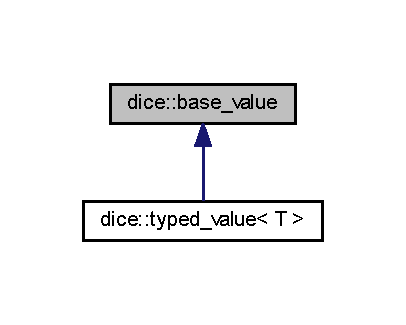
\includegraphics[width=195pt]{classdice_1_1base__value__inherit__graph}
\end{center}
\end{figure}
\subsection*{Public Member Functions}
\begin{DoxyCompactItemize}
\item 
virtual \mbox{\hyperlink{value_8hpp_ab9af7d8ecc381e026ca4d07a745f23eb}{type\+\_\+id}} \mbox{\hyperlink{classdice_1_1base__value_a5125d076b0ed6a398f4f4f8fe19ef60b}{type}} () const =0
\begin{DoxyCompactList}\small\item\em Get type of this value. \end{DoxyCompactList}\item 
virtual std\+::unique\+\_\+ptr$<$ \mbox{\hyperlink{classdice_1_1base__value}{base\+\_\+value}} $>$ \mbox{\hyperlink{classdice_1_1base__value_a58335a522dda6d97332f938ead90aa15}{clone}} () const =0
\begin{DoxyCompactList}\small\item\em Create a copy of this value. \end{DoxyCompactList}\item 
virtual bool \mbox{\hyperlink{classdice_1_1base__value_a81269be4c101eeef6d48810823e1835c}{equals}} (const \mbox{\hyperlink{classdice_1_1base__value}{base\+\_\+value}} \&other) const =0
\begin{DoxyCompactList}\small\item\em Check whether this value is equal to other value. \end{DoxyCompactList}\item 
bool \mbox{\hyperlink{classdice_1_1base__value_a5939b300dd577d307cf94d3a6d726210}{operator==}} (const \mbox{\hyperlink{classdice_1_1base__value}{base\+\_\+value}} \&other) const
\begin{DoxyCompactList}\small\item\em Check whether this value is equal to other value. \end{DoxyCompactList}\item 
bool \mbox{\hyperlink{classdice_1_1base__value_a6a05109afbb4b9a2c77887d76e7edbab}{operator!=}} (const \mbox{\hyperlink{classdice_1_1base__value}{base\+\_\+value}} \&other) const
\begin{DoxyCompactList}\small\item\em Check whether this value is not equal to other value. \end{DoxyCompactList}\item 
virtual void \mbox{\hyperlink{classdice_1_1base__value_a8ab0acd9a7b10035a1c8f8a0f05b40b4}{accept}} (\mbox{\hyperlink{classdice_1_1value__visitor}{value\+\_\+visitor}} $\ast$visitor)=0
\begin{DoxyCompactList}\small\item\em Visit this value using given visitor. \end{DoxyCompactList}\end{DoxyCompactItemize}


\subsection{Detailed Description}
Parent of all value types that are used in dice expressions. 

\subsection{Member Function Documentation}
\mbox{\Hypertarget{classdice_1_1base__value_a8ab0acd9a7b10035a1c8f8a0f05b40b4}\label{classdice_1_1base__value_a8ab0acd9a7b10035a1c8f8a0f05b40b4}} 
\index{dice\+::base\+\_\+value@{dice\+::base\+\_\+value}!accept@{accept}}
\index{accept@{accept}!dice\+::base\+\_\+value@{dice\+::base\+\_\+value}}
\subsubsection{\texorpdfstring{accept()}{accept()}}
{\footnotesize\ttfamily virtual void dice\+::base\+\_\+value\+::accept (\begin{DoxyParamCaption}\item[{\mbox{\hyperlink{classdice_1_1value__visitor}{value\+\_\+visitor}} $\ast$}]{visitor }\end{DoxyParamCaption})\hspace{0.3cm}{\ttfamily [pure virtual]}}



Visit this value using given visitor. 


\begin{DoxyParams}{Parameters}
{\em visitor} & \\
\hline
\end{DoxyParams}


Implemented in \mbox{\hyperlink{classdice_1_1typed__value_ae9563902b664c40a4b3d8a8cb201a194}{dice\+::typed\+\_\+value$<$ T $>$}}.

\mbox{\Hypertarget{classdice_1_1base__value_a58335a522dda6d97332f938ead90aa15}\label{classdice_1_1base__value_a58335a522dda6d97332f938ead90aa15}} 
\index{dice\+::base\+\_\+value@{dice\+::base\+\_\+value}!clone@{clone}}
\index{clone@{clone}!dice\+::base\+\_\+value@{dice\+::base\+\_\+value}}
\subsubsection{\texorpdfstring{clone()}{clone()}}
{\footnotesize\ttfamily virtual std\+::unique\+\_\+ptr$<$\mbox{\hyperlink{classdice_1_1base__value}{base\+\_\+value}}$>$ dice\+::base\+\_\+value\+::clone (\begin{DoxyParamCaption}{ }\end{DoxyParamCaption}) const\hspace{0.3cm}{\ttfamily [pure virtual]}}



Create a copy of this value. 

\begin{DoxyReturn}{Returns}
copied value 
\end{DoxyReturn}


Implemented in \mbox{\hyperlink{classdice_1_1typed__value_a54490141b25b17213989fd2e859b4f59}{dice\+::typed\+\_\+value$<$ T $>$}}.

\mbox{\Hypertarget{classdice_1_1base__value_a81269be4c101eeef6d48810823e1835c}\label{classdice_1_1base__value_a81269be4c101eeef6d48810823e1835c}} 
\index{dice\+::base\+\_\+value@{dice\+::base\+\_\+value}!equals@{equals}}
\index{equals@{equals}!dice\+::base\+\_\+value@{dice\+::base\+\_\+value}}
\subsubsection{\texorpdfstring{equals()}{equals()}}
{\footnotesize\ttfamily virtual bool dice\+::base\+\_\+value\+::equals (\begin{DoxyParamCaption}\item[{const \mbox{\hyperlink{classdice_1_1base__value}{base\+\_\+value}} \&}]{other }\end{DoxyParamCaption}) const\hspace{0.3cm}{\ttfamily [pure virtual]}}



Check whether this value is equal to other value. 


\begin{DoxyParams}{Parameters}
{\em other} & value to compare with this value\\
\hline
\end{DoxyParams}
\begin{DoxyReturn}{Returns}
true iff both have the same type and represent the same value 
\end{DoxyReturn}


Implemented in \mbox{\hyperlink{classdice_1_1typed__value_aeb5c87839a5e3ecb7beac6abc05e6701}{dice\+::typed\+\_\+value$<$ T $>$}}.

\mbox{\Hypertarget{classdice_1_1base__value_a6a05109afbb4b9a2c77887d76e7edbab}\label{classdice_1_1base__value_a6a05109afbb4b9a2c77887d76e7edbab}} 
\index{dice\+::base\+\_\+value@{dice\+::base\+\_\+value}!operator"!=@{operator"!=}}
\index{operator"!=@{operator"!=}!dice\+::base\+\_\+value@{dice\+::base\+\_\+value}}
\subsubsection{\texorpdfstring{operator"!=()}{operator!=()}}
{\footnotesize\ttfamily bool dice\+::base\+\_\+value\+::operator!= (\begin{DoxyParamCaption}\item[{const \mbox{\hyperlink{classdice_1_1base__value}{base\+\_\+value}} \&}]{other }\end{DoxyParamCaption}) const\hspace{0.3cm}{\ttfamily [inline]}}



Check whether this value is not equal to other value. 


\begin{DoxyParams}{Parameters}
{\em other} & value\\
\hline
\end{DoxyParams}
\begin{DoxyReturn}{Returns}
ture iff values are different That is, values or types are different 
\end{DoxyReturn}
\mbox{\Hypertarget{classdice_1_1base__value_a5939b300dd577d307cf94d3a6d726210}\label{classdice_1_1base__value_a5939b300dd577d307cf94d3a6d726210}} 
\index{dice\+::base\+\_\+value@{dice\+::base\+\_\+value}!operator==@{operator==}}
\index{operator==@{operator==}!dice\+::base\+\_\+value@{dice\+::base\+\_\+value}}
\subsubsection{\texorpdfstring{operator==()}{operator==()}}
{\footnotesize\ttfamily bool dice\+::base\+\_\+value\+::operator== (\begin{DoxyParamCaption}\item[{const \mbox{\hyperlink{classdice_1_1base__value}{base\+\_\+value}} \&}]{other }\end{DoxyParamCaption}) const\hspace{0.3cm}{\ttfamily [inline]}}



Check whether this value is equal to other value. 


\begin{DoxyParams}{Parameters}
{\em other} & value (right hand side of the == operator)\\
\hline
\end{DoxyParams}
\begin{DoxyReturn}{Returns}
true iff both have the same type and represent the same value 
\end{DoxyReturn}
\mbox{\Hypertarget{classdice_1_1base__value_a5125d076b0ed6a398f4f4f8fe19ef60b}\label{classdice_1_1base__value_a5125d076b0ed6a398f4f4f8fe19ef60b}} 
\index{dice\+::base\+\_\+value@{dice\+::base\+\_\+value}!type@{type}}
\index{type@{type}!dice\+::base\+\_\+value@{dice\+::base\+\_\+value}}
\subsubsection{\texorpdfstring{type()}{type()}}
{\footnotesize\ttfamily virtual \mbox{\hyperlink{value_8hpp_ab9af7d8ecc381e026ca4d07a745f23eb}{type\+\_\+id}} dice\+::base\+\_\+value\+::type (\begin{DoxyParamCaption}{ }\end{DoxyParamCaption}) const\hspace{0.3cm}{\ttfamily [pure virtual]}}



Get type of this value. 

It has to be unique for each type. It has to be the same for the same type (i.\+e. multiple values of the same type will return the same type id)

\begin{DoxyReturn}{Returns}
type id of the type of this value 
\end{DoxyReturn}


Implemented in \mbox{\hyperlink{classdice_1_1typed__value_aa75a4167e6d3ff2640fd2fa65442e2ed}{dice\+::typed\+\_\+value$<$ T $>$}}.



The documentation for this class was generated from the following file\+:\begin{DoxyCompactItemize}
\item 
C\+:/projects/dice/src/\mbox{\hyperlink{value_8hpp}{value.\+hpp}}\end{DoxyCompactItemize}

\hypertarget{classdice_1_1bernoulli__tag}{}\section{dice\+:\+:bernoulli\+\_\+tag Class Reference}
\label{classdice_1_1bernoulli__tag}\index{dice\+::bernoulli\+\_\+tag@{dice\+::bernoulli\+\_\+tag}}


The documentation for this class was generated from the following file\+:\begin{DoxyCompactItemize}
\item 
C\+:/projects/dice/src/random\+\_\+variable.\+hpp\end{DoxyCompactItemize}

\hypertarget{structdice_1_1calculator}{}\section{dice\+:\+:calculator Struct Reference}
\label{structdice_1_1calculator}\index{dice\+::calculator@{dice\+::calculator}}


Facade for script evaluation.  




{\ttfamily \#include $<$calculator.\+hpp$>$}



Collaboration diagram for dice\+:\+:calculator\+:\nopagebreak
\begin{figure}[H]
\begin{center}
\leavevmode
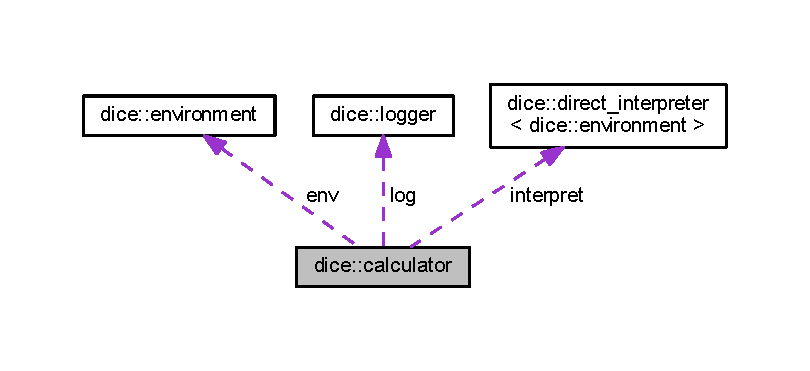
\includegraphics[width=350pt]{structdice_1_1calculator__coll__graph}
\end{center}
\end{figure}
\subsection*{Public Types}
\begin{DoxyCompactItemize}
\item 
\mbox{\Hypertarget{structdice_1_1calculator_a1dd6c840953d7d7a8523b9e3637d61a0}\label{structdice_1_1calculator_a1dd6c840953d7d7a8523b9e3637d61a0}} 
using {\bfseries value\+\_\+list} = std\+::vector$<$ std\+::unique\+\_\+ptr$<$ \mbox{\hyperlink{classdice_1_1base__value}{base\+\_\+value}} $>$ $>$
\end{DoxyCompactItemize}
\subsection*{Public Member Functions}
\begin{DoxyCompactItemize}
\item 
value\+\_\+list \mbox{\hyperlink{structdice_1_1calculator_a63547bad8045470c9849124502036052}{evaluate}} (std\+::istream $\ast$input)
\begin{DoxyCompactList}\small\item\em Evaluate command in given input stream. \end{DoxyCompactList}\item 
value\+\_\+list \mbox{\hyperlink{structdice_1_1calculator_ad1b34884dbf00d5e1e140195e9a50ecc}{evaluate}} (const std\+::string \&command)
\begin{DoxyCompactList}\small\item\em Process command in a string. \end{DoxyCompactList}\item 
void \mbox{\hyperlink{structdice_1_1calculator_a6fe7689c86d8df71f7f312dbd7defdcf}{enable\+\_\+interactive\+\_\+mode}} ()
\begin{DoxyCompactList}\small\item\em Enable interactive mode. \end{DoxyCompactList}\end{DoxyCompactItemize}
\subsection*{Public Attributes}
\begin{DoxyCompactItemize}
\item 
\mbox{\Hypertarget{structdice_1_1calculator_ab9cb5e793d3db99f481b6335c155f193}\label{structdice_1_1calculator_ab9cb5e793d3db99f481b6335c155f193}} 
\mbox{\hyperlink{classdice_1_1logger}{dice\+::logger}} {\bfseries log}
\item 
\mbox{\Hypertarget{structdice_1_1calculator_a88bc893a03a784dd6a5bfeb4583ce60f}\label{structdice_1_1calculator_a88bc893a03a784dd6a5bfeb4583ce60f}} 
\mbox{\hyperlink{classdice_1_1environment}{dice\+::environment}} {\bfseries env}
\item 
\mbox{\Hypertarget{structdice_1_1calculator_a6e029fd9e45e36f4f4b92c7a9df8c3da}\label{structdice_1_1calculator_a6e029fd9e45e36f4f4b92c7a9df8c3da}} 
\mbox{\hyperlink{classdice_1_1direct__interpreter}{dice\+::direct\+\_\+interpreter}}$<$ \mbox{\hyperlink{classdice_1_1environment}{dice\+::environment}} $>$ {\bfseries interpret}
\end{DoxyCompactItemize}


\subsection{Detailed Description}
Facade for script evaluation. 

Example usage\+: 
\begin{DoxyCode}
calculator c;
calculator::value\_list result = c.evaluate(\textcolor{stringliteral}{"1d6"});
\{
     std::ifstrem file\{ \textcolor{stringliteral}{"input.dice"} \};
     result = c.evaluate(&file);
\}
\end{DoxyCode}
 

\subsection{Member Function Documentation}
\mbox{\Hypertarget{structdice_1_1calculator_a6fe7689c86d8df71f7f312dbd7defdcf}\label{structdice_1_1calculator_a6fe7689c86d8df71f7f312dbd7defdcf}} 
\index{dice\+::calculator@{dice\+::calculator}!enable\+\_\+interactive\+\_\+mode@{enable\+\_\+interactive\+\_\+mode}}
\index{enable\+\_\+interactive\+\_\+mode@{enable\+\_\+interactive\+\_\+mode}!dice\+::calculator@{dice\+::calculator}}
\subsubsection{\texorpdfstring{enable\+\_\+interactive\+\_\+mode()}{enable\_interactive\_mode()}}
{\footnotesize\ttfamily void dice\+::calculator\+::enable\+\_\+interactive\+\_\+mode (\begin{DoxyParamCaption}{ }\end{DoxyParamCaption})}



Enable interactive mode. 

Interactive mode is optimized for repeated use of the environment. It allows variable redefinition. \mbox{\Hypertarget{structdice_1_1calculator_a63547bad8045470c9849124502036052}\label{structdice_1_1calculator_a63547bad8045470c9849124502036052}} 
\index{dice\+::calculator@{dice\+::calculator}!evaluate@{evaluate}}
\index{evaluate@{evaluate}!dice\+::calculator@{dice\+::calculator}}
\subsubsection{\texorpdfstring{evaluate()}{evaluate()}\hspace{0.1cm}{\footnotesize\ttfamily [1/2]}}
{\footnotesize\ttfamily dice\+::calculator\+::value\+\_\+list dice\+::calculator\+::evaluate (\begin{DoxyParamCaption}\item[{std\+::istream $\ast$}]{input }\end{DoxyParamCaption})}



Evaluate command in given input stream. 


\begin{DoxyParams}{Parameters}
{\em input} & character stream pointer\\
\hline
\end{DoxyParams}
\begin{DoxyReturn}{Returns}
evaluated values 
\end{DoxyReturn}
\mbox{\Hypertarget{structdice_1_1calculator_ad1b34884dbf00d5e1e140195e9a50ecc}\label{structdice_1_1calculator_ad1b34884dbf00d5e1e140195e9a50ecc}} 
\index{dice\+::calculator@{dice\+::calculator}!evaluate@{evaluate}}
\index{evaluate@{evaluate}!dice\+::calculator@{dice\+::calculator}}
\subsubsection{\texorpdfstring{evaluate()}{evaluate()}\hspace{0.1cm}{\footnotesize\ttfamily [2/2]}}
{\footnotesize\ttfamily dice\+::calculator\+::value\+\_\+list dice\+::calculator\+::evaluate (\begin{DoxyParamCaption}\item[{const std\+::string \&}]{command }\end{DoxyParamCaption})}



Process command in a string. 


\begin{DoxyParams}{Parameters}
{\em command} & as a string\\
\hline
\end{DoxyParams}
\begin{DoxyReturn}{Returns}
evaluated values 
\end{DoxyReturn}


The documentation for this struct was generated from the following files\+:\begin{DoxyCompactItemize}
\item 
C\+:/projects/dice/src/calculator.\+hpp\item 
C\+:/projects/dice/src/calculator.\+cpp\end{DoxyCompactItemize}

\hypertarget{structcommand__reader}{}\section{command\+\_\+reader Struct Reference}
\label{structcommand__reader}\index{command\+\_\+reader@{command\+\_\+reader}}
\subsection*{Public Member Functions}
\begin{DoxyCompactItemize}
\item 
bool \mbox{\hyperlink{structcommand__reader_aefd772702c6cca30efb2a932910e51cc}{try\+\_\+read}} (std\+::string \&out\+\_\+line)
\begin{DoxyCompactList}\small\item\em Read line from the input. \end{DoxyCompactList}\end{DoxyCompactItemize}


\subsection{Member Function Documentation}
\mbox{\Hypertarget{structcommand__reader_aefd772702c6cca30efb2a932910e51cc}\label{structcommand__reader_aefd772702c6cca30efb2a932910e51cc}} 
\index{command\+\_\+reader@{command\+\_\+reader}!try\+\_\+read@{try\+\_\+read}}
\index{try\+\_\+read@{try\+\_\+read}!command\+\_\+reader@{command\+\_\+reader}}
\subsubsection{\texorpdfstring{try\+\_\+read()}{try\_read()}}
{\footnotesize\ttfamily bool command\+\_\+reader\+::try\+\_\+read (\begin{DoxyParamCaption}\item[{std\+::string \&}]{out\+\_\+line }\end{DoxyParamCaption})\hspace{0.3cm}{\ttfamily [inline]}}



Read line from the input. 

The line is saved to history. 
\begin{DoxyParams}{Parameters}
{\em out\+\_\+line} & read line \\
\hline
\end{DoxyParams}
\begin{DoxyReturn}{Returns}
ture iff we should continue reading 
\end{DoxyReturn}


The documentation for this struct was generated from the following file\+:\begin{DoxyCompactItemize}
\item 
C\+:/projects/dice/src/main.\+cpp\end{DoxyCompactItemize}

\hypertarget{classdice_1_1compiler__error}{}\section{dice\+:\+:compiler\+\_\+error Class Reference}
\label{classdice_1_1compiler__error}\index{dice\+::compiler\+\_\+error@{dice\+::compiler\+\_\+error}}


An error thrown when there is an error in computation during script evaluation.  




{\ttfamily \#include $<$environment.\+hpp$>$}



Inheritance diagram for dice\+:\+:compiler\+\_\+error\+:\nopagebreak
\begin{figure}[H]
\begin{center}
\leavevmode
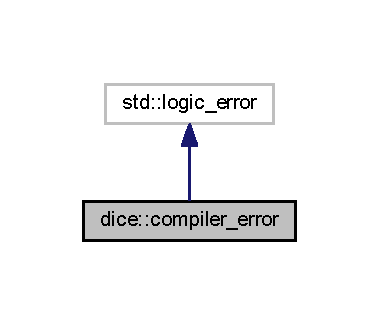
\includegraphics[width=182pt]{classdice_1_1compiler__error__inherit__graph}
\end{center}
\end{figure}


Collaboration diagram for dice\+:\+:compiler\+\_\+error\+:\nopagebreak
\begin{figure}[H]
\begin{center}
\leavevmode
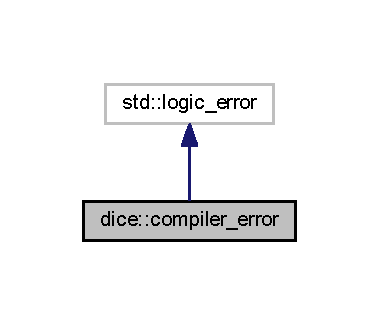
\includegraphics[width=182pt]{classdice_1_1compiler__error__coll__graph}
\end{center}
\end{figure}
\subsection*{Public Member Functions}
\begin{DoxyCompactItemize}
\item 
\mbox{\Hypertarget{classdice_1_1compiler__error_addf72d1445219a85eb03321721a78bdf}\label{classdice_1_1compiler__error_addf72d1445219a85eb03321721a78bdf}} 
{\bfseries compiler\+\_\+error} (const std\+::string \&message)
\end{DoxyCompactItemize}


\subsection{Detailed Description}
An error thrown when there is an error in computation during script evaluation. 

The documentation for this class was generated from the following file\+:\begin{DoxyCompactItemize}
\item 
C\+:/projects/dice/src/environment.\+hpp\end{DoxyCompactItemize}

\hypertarget{classdice_1_1constant__tag}{}\section{dice\+:\+:constant\+\_\+tag Class Reference}
\label{classdice_1_1constant__tag}\index{dice\+::constant\+\_\+tag@{dice\+::constant\+\_\+tag}}


The documentation for this class was generated from the following file\+:\begin{DoxyCompactItemize}
\item 
C\+:/projects/dice/src/random\+\_\+variable.\+hpp\end{DoxyCompactItemize}

\hypertarget{classdice_1_1conversion__visitor}{}\section{dice\+:\+:conversion\+\_\+visitor Class Reference}
\label{classdice_1_1conversion__visitor}\index{dice\+::conversion\+\_\+visitor@{dice\+::conversion\+\_\+visitor}}


Inheritance diagram for dice\+:\+:conversion\+\_\+visitor\+:\nopagebreak
\begin{figure}[H]
\begin{center}
\leavevmode
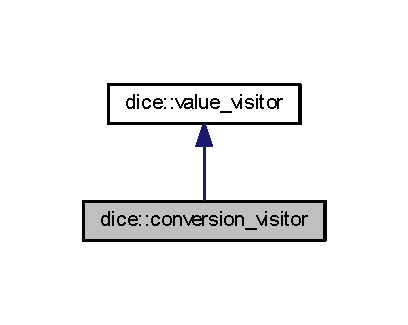
\includegraphics[width=196pt]{classdice_1_1conversion__visitor__inherit__graph}
\end{center}
\end{figure}


Collaboration diagram for dice\+:\+:conversion\+\_\+visitor\+:\nopagebreak
\begin{figure}[H]
\begin{center}
\leavevmode
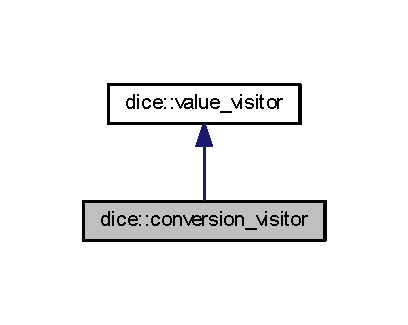
\includegraphics[width=196pt]{classdice_1_1conversion__visitor__coll__graph}
\end{center}
\end{figure}
\subsection*{Public Types}
\begin{DoxyCompactItemize}
\item 
\mbox{\Hypertarget{classdice_1_1conversion__visitor_ac5411140c63f70a70f216437175627c2}\label{classdice_1_1conversion__visitor_ac5411140c63f70a70f216437175627c2}} 
using {\bfseries value\+\_\+type} = std\+::unique\+\_\+ptr$<$ \mbox{\hyperlink{classdice_1_1base__value}{base\+\_\+value}} $>$
\end{DoxyCompactItemize}
\subsection*{Public Member Functions}
\begin{DoxyCompactItemize}
\item 
\mbox{\Hypertarget{classdice_1_1conversion__visitor_a3014ecef08b8d88161ad9fb654ce6abd}\label{classdice_1_1conversion__visitor_a3014ecef08b8d88161ad9fb654ce6abd}} 
{\bfseries conversion\+\_\+visitor} (\mbox{\hyperlink{value_8hpp_ab9af7d8ecc381e026ca4d07a745f23eb}{type\+\_\+id}} result\+\_\+type)
\item 
\mbox{\Hypertarget{classdice_1_1conversion__visitor_aba40c0192bb5122ea8db7abb0e79b53d}\label{classdice_1_1conversion__visitor_aba40c0192bb5122ea8db7abb0e79b53d}} 
void {\bfseries visit} (\mbox{\hyperlink{classdice_1_1typed__value}{type\+\_\+int}} $\ast$value) override
\item 
\mbox{\Hypertarget{classdice_1_1conversion__visitor_a4ea9bf6bba994f6c7bcb9ea7ebfb842d}\label{classdice_1_1conversion__visitor_a4ea9bf6bba994f6c7bcb9ea7ebfb842d}} 
void {\bfseries visit} (\mbox{\hyperlink{classdice_1_1typed__value}{type\+\_\+real}} $\ast$) override
\item 
\mbox{\Hypertarget{classdice_1_1conversion__visitor_a4d136c9ea1d54dba2e194fd26aa56a91}\label{classdice_1_1conversion__visitor_a4d136c9ea1d54dba2e194fd26aa56a91}} 
void {\bfseries visit} (\mbox{\hyperlink{classdice_1_1typed__value}{type\+\_\+rand\+\_\+var}} $\ast$) override
\item 
\mbox{\Hypertarget{classdice_1_1conversion__visitor_ae0bbbe753e8800d5dd0b4636c8de203b}\label{classdice_1_1conversion__visitor_ae0bbbe753e8800d5dd0b4636c8de203b}} 
value\+\_\+type {\bfseries value} ()
\end{DoxyCompactItemize}


The documentation for this class was generated from the following files\+:\begin{DoxyCompactItemize}
\item 
C\+:/projects/dice/src/conversions.\+hpp\item 
C\+:/projects/dice/src/conversions.\+cpp\end{DoxyCompactItemize}

\hypertarget{classdice_1_1conversions}{}\section{dice\+:\+:conversions Class Reference}
\label{classdice_1_1conversions}\index{dice\+::conversions@{dice\+::conversions}}


This class manages conversions of values in dice expression.  




{\ttfamily \#include $<$conversions.\+hpp$>$}

\subsection*{Public Types}
\begin{DoxyCompactItemize}
\item 
\mbox{\Hypertarget{classdice_1_1conversions_afa76a68a1fb1140608ba48da6f7bc0bd}\label{classdice_1_1conversions_afa76a68a1fb1140608ba48da6f7bc0bd}} 
using {\bfseries value\+\_\+type} = std\+::unique\+\_\+ptr$<$ \mbox{\hyperlink{classdice_1_1base__value}{base\+\_\+value}} $>$
\item 
\mbox{\Hypertarget{classdice_1_1conversions_a62ec635e5e7832c05bf351dae4b135e4}\label{classdice_1_1conversions_a62ec635e5e7832c05bf351dae4b135e4}} 
using {\bfseries cost\+\_\+type} = std\+::size\+\_\+t
\end{DoxyCompactItemize}
\subsection*{Public Member Functions}
\begin{DoxyCompactItemize}
\item 
cost\+\_\+type \mbox{\hyperlink{classdice_1_1conversions_adbc4f917f240f7ab4440cfc7d81e6250}{cost}} (\mbox{\hyperlink{value_8hpp_ab9af7d8ecc381e026ca4d07a745f23eb}{type\+\_\+id}} from, \mbox{\hyperlink{value_8hpp_ab9af7d8ecc381e026ca4d07a745f23eb}{type\+\_\+id}} to) const
\begin{DoxyCompactList}\small\item\em Find conversion cost from type {\ttfamily from} to type {\ttfamily to}. \end{DoxyCompactList}\item 
value\+\_\+type \mbox{\hyperlink{classdice_1_1conversions_ab6a95940f7c218a4e610a81b9b838291}{convert}} (\mbox{\hyperlink{value_8hpp_ab9af7d8ecc381e026ca4d07a745f23eb}{type\+\_\+id}} to, value\+\_\+type value) const
\begin{DoxyCompactList}\small\item\em Convert value to type {\ttfamily to}. \end{DoxyCompactList}\end{DoxyCompactItemize}
\subsection*{Static Public Attributes}
\begin{DoxyCompactItemize}
\item 
static const cost\+\_\+type {\bfseries max\+\_\+cost}
\end{DoxyCompactItemize}


\subsection{Detailed Description}
This class manages conversions of values in dice expression. 

Example usage\+: 
\begin{DoxyCode}
conversions c;
conversions::cost\_type cost\_int\_to\_real = c.cost(type\_id::integer, type\_id::real);
conversions::value\_type real\_value = c.convert(type\_id::real, make<type\_int>(14));
\end{DoxyCode}
 

\subsection{Member Function Documentation}
\mbox{\Hypertarget{classdice_1_1conversions_ab6a95940f7c218a4e610a81b9b838291}\label{classdice_1_1conversions_ab6a95940f7c218a4e610a81b9b838291}} 
\index{dice\+::conversions@{dice\+::conversions}!convert@{convert}}
\index{convert@{convert}!dice\+::conversions@{dice\+::conversions}}
\subsubsection{\texorpdfstring{convert()}{convert()}}
{\footnotesize\ttfamily dice\+::conversions\+::value\+\_\+type dice\+::conversions\+::convert (\begin{DoxyParamCaption}\item[{\mbox{\hyperlink{value_8hpp_ab9af7d8ecc381e026ca4d07a745f23eb}{type\+\_\+id}}}]{to,  }\item[{value\+\_\+type}]{value }\end{DoxyParamCaption}) const}



Convert value to type {\ttfamily to}. 


\begin{DoxyParams}{Parameters}
{\em to} & type id \\
\hline
{\em value} & to convert\\
\hline
\end{DoxyParams}
\begin{DoxyReturn}{Returns}
converted value 
\end{DoxyReturn}
\mbox{\Hypertarget{classdice_1_1conversions_adbc4f917f240f7ab4440cfc7d81e6250}\label{classdice_1_1conversions_adbc4f917f240f7ab4440cfc7d81e6250}} 
\index{dice\+::conversions@{dice\+::conversions}!cost@{cost}}
\index{cost@{cost}!dice\+::conversions@{dice\+::conversions}}
\subsubsection{\texorpdfstring{cost()}{cost()}}
{\footnotesize\ttfamily dice\+::conversions\+::cost\+\_\+type dice\+::conversions\+::cost (\begin{DoxyParamCaption}\item[{\mbox{\hyperlink{value_8hpp_ab9af7d8ecc381e026ca4d07a745f23eb}{type\+\_\+id}}}]{from,  }\item[{\mbox{\hyperlink{value_8hpp_ab9af7d8ecc381e026ca4d07a745f23eb}{type\+\_\+id}}}]{to }\end{DoxyParamCaption}) const}



Find conversion cost from type {\ttfamily from} to type {\ttfamily to}. 


\begin{DoxyParams}{Parameters}
{\em from} & type id \\
\hline
{\em to} & type id\\
\hline
\end{DoxyParams}
\begin{DoxyReturn}{Returns}
cost of the conversion. 0 =$>$ no conversion needed, max\+\_\+cost =$>$ the conversion is not supported 
\end{DoxyReturn}


\subsection{Member Data Documentation}
\mbox{\Hypertarget{classdice_1_1conversions_ad0c8e703408d6a936ee83f8f31e8512b}\label{classdice_1_1conversions_ad0c8e703408d6a936ee83f8f31e8512b}} 
\index{dice\+::conversions@{dice\+::conversions}!max\+\_\+cost@{max\+\_\+cost}}
\index{max\+\_\+cost@{max\+\_\+cost}!dice\+::conversions@{dice\+::conversions}}
\subsubsection{\texorpdfstring{max\+\_\+cost}{max\_cost}}
{\footnotesize\ttfamily const dice\+::conversions\+::cost\+\_\+type dice\+::conversions\+::max\+\_\+cost\hspace{0.3cm}{\ttfamily [static]}}

{\bfseries Initial value\+:}
\begin{DoxyCode}
= 
    std::numeric\_limits<dice::conversions::cost\_type>::max()
\end{DoxyCode}


The documentation for this class was generated from the following files\+:\begin{DoxyCompactItemize}
\item 
C\+:/projects/dice/src/conversions.\+hpp\item 
C\+:/projects/dice/src/conversions.\+cpp\end{DoxyCompactItemize}

\hypertarget{classdice_1_1decomposition}{}\section{dice\+:\+:decomposition$<$ Value\+Type, Probability\+Type $>$ Class Template Reference}
\label{classdice_1_1decomposition}\index{dice\+::decomposition$<$ Value\+Type, Probability\+Type $>$@{dice\+::decomposition$<$ Value\+Type, Probability\+Type $>$}}


Object representing a decomposition of a function of random variables.  




{\ttfamily \#include $<$decomposition.\+hpp$>$}

\subsection*{Public Types}
\begin{DoxyCompactItemize}
\item 
\mbox{\Hypertarget{classdice_1_1decomposition_a943670b415a813c050db79c9430d0955}\label{classdice_1_1decomposition_a943670b415a813c050db79c9430d0955}} 
using {\bfseries var\+\_\+type} = \mbox{\hyperlink{classdice_1_1random__variable}{random\+\_\+variable}}$<$ Value\+Type, Probability\+Type $>$
\item 
\mbox{\Hypertarget{classdice_1_1decomposition_a891387c501eb8b627b5338730f9cf60d}\label{classdice_1_1decomposition_a891387c501eb8b627b5338730f9cf60d}} 
using {\bfseries probability\+\_\+iterator} = \mbox{\hyperlink{classdice_1_1decomposition__iterator}{decomposition\+\_\+iterator}}$<$ Value\+Type, Probability\+Type $>$
\item 
\mbox{\Hypertarget{classdice_1_1decomposition_aa467b1cad750472097497a3040c7eae5}\label{classdice_1_1decomposition_aa467b1cad750472097497a3040c7eae5}} 
using {\bfseries value\+\_\+type} = Value\+Type
\item 
\mbox{\Hypertarget{classdice_1_1decomposition_a74ab5f6f91589c64a5555516ca3edf1f}\label{classdice_1_1decomposition_a74ab5f6f91589c64a5555516ca3edf1f}} 
using {\bfseries probability\+\_\+type} = Probability\+Type
\item 
\mbox{\Hypertarget{classdice_1_1decomposition_a363def968319171903bb449262f2a4c3}\label{classdice_1_1decomposition_a363def968319171903bb449262f2a4c3}} 
using {\bfseries frequency\+\_\+list} = typename var\+\_\+type\+::frequency\+\_\+list
\item 
\mbox{\Hypertarget{classdice_1_1decomposition_a4d441672f3a0864e416fb109f42c167b}\label{classdice_1_1decomposition_a4d441672f3a0864e416fb109f42c167b}} 
using {\bfseries probability\+\_\+list} = typename var\+\_\+type\+::probability\+\_\+list
\end{DoxyCompactItemize}
\subsection*{Public Member Functions}
\begin{DoxyCompactItemize}
\item 
\mbox{\hyperlink{classdice_1_1decomposition_a0ec6a2cfb52048bd1e553d53627aec2c}{decomposition}} (const \mbox{\hyperlink{classdice_1_1random__variable}{var\+\_\+type}} \&variable)
\begin{DoxyCompactList}\small\item\em Create decomposition from \mbox{\hyperlink{classdice_1_1random__variable}{random\+\_\+variable}}. \end{DoxyCompactList}\item 
\mbox{\hyperlink{classdice_1_1decomposition_a1c0f335542198fe9f6ca6d0a0c2a4de0}{decomposition}} (\mbox{\hyperlink{classdice_1_1random__variable}{var\+\_\+type}} \&\&variable)
\begin{DoxyCompactList}\small\item\em Create decomposition from \mbox{\hyperlink{classdice_1_1random__variable}{random\+\_\+variable}}. \end{DoxyCompactList}\item 
\mbox{\Hypertarget{classdice_1_1decomposition_ad44e439c795cfd2c881602cea4ed99cb}\label{classdice_1_1decomposition_ad44e439c795cfd2c881602cea4ed99cb}} 
{\bfseries decomposition} (std\+::vector$<$ std\+::pair$<$ value\+\_\+type, std\+::size\+\_\+t $>$$>$ \&\&list)
\item 
\mbox{\Hypertarget{classdice_1_1decomposition_af0af395a0462070a80bff39ed6a8e4e5}\label{classdice_1_1decomposition_af0af395a0462070a80bff39ed6a8e4e5}} 
{\bfseries decomposition} (\mbox{\hyperlink{classdice_1_1bernoulli__tag}{bernoulli\+\_\+tag}}, Probability\+Type success)
\item 
\mbox{\Hypertarget{classdice_1_1decomposition_a96000e52a4ac3c777ccae25eced198cf}\label{classdice_1_1decomposition_a96000e52a4ac3c777ccae25eced198cf}} 
{\bfseries decomposition} (\mbox{\hyperlink{classdice_1_1constant__tag}{constant\+\_\+tag}}, value\+\_\+type value)
\item 
\mbox{\Hypertarget{classdice_1_1decomposition_abe2edcf9ec724d7300cefa21132dd8c1}\label{classdice_1_1decomposition_abe2edcf9ec724d7300cefa21132dd8c1}} 
{\bfseries decomposition} (const \mbox{\hyperlink{classdice_1_1decomposition}{decomposition}} \&)=default
\item 
\mbox{\Hypertarget{classdice_1_1decomposition_a08552602e4e040eb8188675a886a3dd5}\label{classdice_1_1decomposition_a08552602e4e040eb8188675a886a3dd5}} 
\mbox{\hyperlink{classdice_1_1decomposition}{decomposition}} \& {\bfseries operator=} (const \mbox{\hyperlink{classdice_1_1decomposition}{decomposition}} \&)=default
\item 
\mbox{\Hypertarget{classdice_1_1decomposition_a7ca52a332c2a05642b24217607817236}\label{classdice_1_1decomposition_a7ca52a332c2a05642b24217607817236}} 
{\bfseries decomposition} (\mbox{\hyperlink{classdice_1_1decomposition}{decomposition}} \&\&)=default
\item 
\mbox{\Hypertarget{classdice_1_1decomposition_a40cd320a0a5ba77cca1066f298c94d97}\label{classdice_1_1decomposition_a40cd320a0a5ba77cca1066f298c94d97}} 
\mbox{\hyperlink{classdice_1_1decomposition}{decomposition}} \& {\bfseries operator=} (\mbox{\hyperlink{classdice_1_1decomposition}{decomposition}} \&\&)=default
\item 
auto \mbox{\hyperlink{classdice_1_1decomposition_abfd6869629c7622d95333dafd9d15cd5}{operator+}} (const \mbox{\hyperlink{classdice_1_1decomposition}{decomposition}} \&other) const
\begin{DoxyCompactList}\small\item\em Compute sum of 2 random variables. \end{DoxyCompactList}\item 
auto \mbox{\hyperlink{classdice_1_1decomposition_ae6bf072b8ba3615e85c3db38e5d78b4f}{operator-\/}} (const \mbox{\hyperlink{classdice_1_1decomposition}{decomposition}} \&other) const
\begin{DoxyCompactList}\small\item\em Subtract other random variable from this. \end{DoxyCompactList}\item 
auto \mbox{\hyperlink{classdice_1_1decomposition_ad9621b64c8ff2679a5a5df4e30561c31}{operator$\ast$}} (const \mbox{\hyperlink{classdice_1_1decomposition}{decomposition}} \&other) const
\begin{DoxyCompactList}\small\item\em Compute product of 2 random variables. \end{DoxyCompactList}\item 
auto \mbox{\hyperlink{classdice_1_1decomposition_ad7e95a376d87a8440ff4ebb4445b264a}{operator/}} (const \mbox{\hyperlink{classdice_1_1decomposition}{decomposition}} \&other) const
\begin{DoxyCompactList}\small\item\em Divide this variable by other variable. \end{DoxyCompactList}\item 
auto \mbox{\hyperlink{classdice_1_1decomposition_a8d70dd95d1923cfb4b7b41d47dd43f33}{operator-\/}} () const
\begin{DoxyCompactList}\small\item\em Multiply this random variable with -\/1. \end{DoxyCompactList}\item 
auto \mbox{\hyperlink{classdice_1_1decomposition_a9ba902091f71d0e6beffc20e9fdcbc80}{less\+\_\+than}} (const \mbox{\hyperlink{classdice_1_1decomposition}{decomposition}} \&other) const
\begin{DoxyCompactList}\small\item\em Compute indicator\+: A $<$ B (where A is this random variale). \end{DoxyCompactList}\item 
auto \mbox{\hyperlink{classdice_1_1decomposition_a64f50038f58aafaba4c328dc07dae9ba}{less\+\_\+than\+\_\+or\+\_\+equal}} (const \mbox{\hyperlink{classdice_1_1decomposition}{decomposition}} \&other) const
\begin{DoxyCompactList}\small\item\em Compute indicator\+: A $<$= B (where A is this random variale). \end{DoxyCompactList}\item 
auto \mbox{\hyperlink{classdice_1_1decomposition_af8a3775b00001f174b9532434a0daad1}{equal}} (const \mbox{\hyperlink{classdice_1_1decomposition}{decomposition}} \&other) const
\begin{DoxyCompactList}\small\item\em Compute indicator\+: A = B (where A is this random variale). \end{DoxyCompactList}\item 
auto \mbox{\hyperlink{classdice_1_1decomposition_a648709e5232534308779c489bc985cc9}{not\+\_\+equal}} (const \mbox{\hyperlink{classdice_1_1decomposition}{decomposition}} \&other) const
\begin{DoxyCompactList}\small\item\em Compute indicator\+: A != B (where A is this random variale). \end{DoxyCompactList}\item 
auto \mbox{\hyperlink{classdice_1_1decomposition_abede851d76806d165ed11861c8ef33ea}{greater\+\_\+than}} (const \mbox{\hyperlink{classdice_1_1decomposition}{decomposition}} \&other) const
\begin{DoxyCompactList}\small\item\em Compute indicator\+: A $>$ B (where A is this random variale). \end{DoxyCompactList}\item 
auto \mbox{\hyperlink{classdice_1_1decomposition_a0f65f2184d050b75bc45b13e5b01b53b}{greater\+\_\+than\+\_\+or\+\_\+equal}} (const \mbox{\hyperlink{classdice_1_1decomposition}{decomposition}} \&other) const
\begin{DoxyCompactList}\small\item\em Compute indicator\+: A $>$= B (where A is this random variale). \end{DoxyCompactList}\item 
{\footnotesize template$<$typename T $>$ }\\auto \mbox{\hyperlink{classdice_1_1decomposition_a39d3bb536e99cd66b2e1c8a0a7a0edc6}{in}} (const T \&lower\+\_\+bound, const T \&upper\+\_\+bound) const
\begin{DoxyCompactList}\small\item\em Compute indicator\+: A in \mbox{[}a, b\mbox{]} (where A is this random variable). \end{DoxyCompactList}\item 
auto \mbox{\hyperlink{classdice_1_1decomposition_afac577e983fb2d45591c536e1741f3d8}{expected\+\_\+value}} () const
\begin{DoxyCompactList}\small\item\em Compute expected value of this random variable. \end{DoxyCompactList}\item 
auto \mbox{\hyperlink{classdice_1_1decomposition_ac4ea31f289d9f6bc4567803fba5949ee}{variance}} () const
\begin{DoxyCompactList}\small\item\em Compute variance of this random variable. \end{DoxyCompactList}\item 
auto \mbox{\hyperlink{classdice_1_1decomposition_a0266f65d4898f049792543b3d52dda86}{deviation}} () const
\begin{DoxyCompactList}\small\item\em Compute standard deviation of this random variable. \end{DoxyCompactList}\item 
auto \mbox{\hyperlink{classdice_1_1decomposition_a43d4eaeae0ad22bf478025cf64bbdfe8}{quantile}} (Probability\+Type probability) const
\begin{DoxyCompactList}\small\item\em Compute quantile of this random variable. \end{DoxyCompactList}\item 
{\footnotesize template$<$typename Variable\+Combination\+Function $>$ }\\auto \mbox{\hyperlink{classdice_1_1decomposition_a323d8d184660b6e8751970002ae850a7}{combine}} (const \mbox{\hyperlink{classdice_1_1decomposition}{decomposition}} \&other, Variable\+Combination\+Function combination) const
\begin{DoxyCompactList}\small\item\em Compute function of 2 random variables\+: A and B. \end{DoxyCompactList}\item 
\mbox{\hyperlink{classdice_1_1random__variable}{var\+\_\+type}} \mbox{\hyperlink{classdice_1_1decomposition_a3483a1060e900dceae13fb73c927889b}{to\+\_\+random\+\_\+variable}} () const
\begin{DoxyCompactList}\small\item\em Convert this decomposition to basic random variable. \end{DoxyCompactList}\item 
bool \mbox{\hyperlink{classdice_1_1decomposition_aa3fe4f89f0ae6361889272ee098c02a8}{has\+\_\+dependencies}} () const
\begin{DoxyCompactList}\small\item\em Check whether this decomposition depends on other random variables. \end{DoxyCompactList}\item 
auto \mbox{\hyperlink{classdice_1_1decomposition_a0daca40a4952466df7e5ebe10f6a37b4}{compute\+\_\+decomposition}} () const
\begin{DoxyCompactList}\small\item\em Compute the decomposition of this random variable. \end{DoxyCompactList}\item 
bool \mbox{\hyperlink{classdice_1_1decomposition_ae3431215ee061fd0db5d578e270b0888}{operator==}} (const \mbox{\hyperlink{classdice_1_1decomposition}{decomposition}} \&other) const
\begin{DoxyCompactList}\small\item\em Check whether this is exactly equal to other decomposition. \end{DoxyCompactList}\item 
\mbox{\Hypertarget{classdice_1_1decomposition_a32db2cb923d2f871138e4487c21d4c01}\label{classdice_1_1decomposition_a32db2cb923d2f871138e4487c21d4c01}} 
bool {\bfseries operator!=} (const \mbox{\hyperlink{classdice_1_1decomposition}{decomposition}} \&other) const
\item 
\mbox{\Hypertarget{classdice_1_1decomposition_a99d601ed8bbc44e32dbdb7dcdff83408}\label{classdice_1_1decomposition_a99d601ed8bbc44e32dbdb7dcdff83408}} 
auto {\bfseries begin} () const
\item 
\mbox{\Hypertarget{classdice_1_1decomposition_ac5cd5b4057b2767169290e86423349a1}\label{classdice_1_1decomposition_ac5cd5b4057b2767169290e86423349a1}} 
auto {\bfseries end} () const
\item 
\mbox{\Hypertarget{classdice_1_1decomposition_acf86c5c07f567d3ee95407e5c8dd788a}\label{classdice_1_1decomposition_acf86c5c07f567d3ee95407e5c8dd788a}} 
std\+::size\+\_\+t {\bfseries size} () const
\item 
\mbox{\Hypertarget{classdice_1_1decomposition_a986e5e2240ec1553cd2370d235e42a21}\label{classdice_1_1decomposition_a986e5e2240ec1553cd2370d235e42a21}} 
auto \& {\bfseries variables\+\_\+internal} ()
\item 
\mbox{\Hypertarget{classdice_1_1decomposition_ac68a42128dd2b20aa41a7826effd06a2}\label{classdice_1_1decomposition_ac68a42128dd2b20aa41a7826effd06a2}} 
auto \& {\bfseries dependencies\+\_\+internal} ()
\end{DoxyCompactItemize}
\subsection*{Friends}
\begin{DoxyCompactItemize}
\item 
\mbox{\Hypertarget{classdice_1_1decomposition_a90f425f8bf994cdc21610c6926c41a92}\label{classdice_1_1decomposition_a90f425f8bf994cdc21610c6926c41a92}} 
class {\bfseries decomposition\+\_\+iterator$<$ Value\+Type, Probability\+Type $>$}
\item 
auto \mbox{\hyperlink{classdice_1_1decomposition_a0c852d5e74d719a95d3056fb79e0a703}{roll}} (const \mbox{\hyperlink{classdice_1_1decomposition}{decomposition}} \&num\+\_\+rolls, const \mbox{\hyperlink{classdice_1_1decomposition}{decomposition}} \&num\+\_\+sides)
\begin{DoxyCompactList}\small\item\em Roll num\+\_\+rolls times with a dice of num\+\_\+sides. \end{DoxyCompactList}\end{DoxyCompactItemize}


\subsection{Detailed Description}
\subsubsection*{template$<$typename Value\+Type, typename Probability\+Type$>$\newline
class dice\+::decomposition$<$ Value\+Type, Probability\+Type $>$}

Object representing a decomposition of a function of random variables. 

It is an adapter for \mbox{\hyperlink{classdice_1_1random__variable}{random\+\_\+variable}}.

It uses the Law of total probability to decompose varibales to conditional variables which are then treated as independent.

Variables are organized in a tree structure. Only leaf nodes are stored in the vars\+\_\+ list. Inner nodes are implicitly given by the deps\+\_\+ list. Each variable in the deps\+\_\+ list corresponds to a level of this tree.

An inner node in this tree is a random variable. It has children corresponding to its values. For example\+: a random variable whose values are 1 or 2 whould have 2 children labeled 1 and 2. A leaf node is a random variable without children nodes.


\begin{DoxyTemplParams}{Template Parameters}
{\em Value\+Type} & type of a value (same as in \mbox{\hyperlink{classdice_1_1random__variable}{random\+\_\+variable}}) \\
\hline
{\em Probability\+Type} & type of probability (same as in \mbox{\hyperlink{classdice_1_1random__variable}{random\+\_\+variable}})\\
\hline
\end{DoxyTemplParams}
\begin{DoxySeeAlso}{See also}
\mbox{\hyperlink{classdice_1_1random__variable}{random\+\_\+variable}} 
\end{DoxySeeAlso}


\subsection{Constructor \& Destructor Documentation}
\mbox{\Hypertarget{classdice_1_1decomposition_a0ec6a2cfb52048bd1e553d53627aec2c}\label{classdice_1_1decomposition_a0ec6a2cfb52048bd1e553d53627aec2c}} 
\index{dice\+::decomposition@{dice\+::decomposition}!decomposition@{decomposition}}
\index{decomposition@{decomposition}!dice\+::decomposition@{dice\+::decomposition}}
\subsubsection{\texorpdfstring{decomposition()}{decomposition()}\hspace{0.1cm}{\footnotesize\ttfamily [1/2]}}
{\footnotesize\ttfamily template$<$typename Value\+Type , typename Probability\+Type $>$ \\
\mbox{\hyperlink{classdice_1_1decomposition}{dice\+::decomposition}}$<$ Value\+Type, Probability\+Type $>$\+::\mbox{\hyperlink{classdice_1_1decomposition}{decomposition}} (\begin{DoxyParamCaption}\item[{const \mbox{\hyperlink{classdice_1_1random__variable}{var\+\_\+type}} \&}]{variable }\end{DoxyParamCaption})\hspace{0.3cm}{\ttfamily [inline]}, {\ttfamily [explicit]}}



Create decomposition from \mbox{\hyperlink{classdice_1_1random__variable}{random\+\_\+variable}}. 


\begin{DoxyParams}{Parameters}
{\em variable} & random variable \\
\hline
\end{DoxyParams}
\mbox{\Hypertarget{classdice_1_1decomposition_a1c0f335542198fe9f6ca6d0a0c2a4de0}\label{classdice_1_1decomposition_a1c0f335542198fe9f6ca6d0a0c2a4de0}} 
\index{dice\+::decomposition@{dice\+::decomposition}!decomposition@{decomposition}}
\index{decomposition@{decomposition}!dice\+::decomposition@{dice\+::decomposition}}
\subsubsection{\texorpdfstring{decomposition()}{decomposition()}\hspace{0.1cm}{\footnotesize\ttfamily [2/2]}}
{\footnotesize\ttfamily template$<$typename Value\+Type , typename Probability\+Type $>$ \\
\mbox{\hyperlink{classdice_1_1decomposition}{dice\+::decomposition}}$<$ Value\+Type, Probability\+Type $>$\+::\mbox{\hyperlink{classdice_1_1decomposition}{decomposition}} (\begin{DoxyParamCaption}\item[{\mbox{\hyperlink{classdice_1_1random__variable}{var\+\_\+type}} \&\&}]{variable }\end{DoxyParamCaption})\hspace{0.3cm}{\ttfamily [inline]}, {\ttfamily [explicit]}}



Create decomposition from \mbox{\hyperlink{classdice_1_1random__variable}{random\+\_\+variable}}. 


\begin{DoxyParams}{Parameters}
{\em variable} & random variable \\
\hline
\end{DoxyParams}


\subsection{Member Function Documentation}
\mbox{\Hypertarget{classdice_1_1decomposition_a323d8d184660b6e8751970002ae850a7}\label{classdice_1_1decomposition_a323d8d184660b6e8751970002ae850a7}} 
\index{dice\+::decomposition@{dice\+::decomposition}!combine@{combine}}
\index{combine@{combine}!dice\+::decomposition@{dice\+::decomposition}}
\subsubsection{\texorpdfstring{combine()}{combine()}}
{\footnotesize\ttfamily template$<$typename Value\+Type , typename Probability\+Type $>$ \\
template$<$typename Variable\+Combination\+Function $>$ \\
auto \mbox{\hyperlink{classdice_1_1decomposition}{dice\+::decomposition}}$<$ Value\+Type, Probability\+Type $>$\+::combine (\begin{DoxyParamCaption}\item[{const \mbox{\hyperlink{classdice_1_1decomposition}{decomposition}}$<$ Value\+Type, Probability\+Type $>$ \&}]{other,  }\item[{Variable\+Combination\+Function}]{combination }\end{DoxyParamCaption}) const\hspace{0.3cm}{\ttfamily [inline]}}



Compute function of 2 random variables\+: A and B. 

Variables does not need to be independent.


\begin{DoxyTemplParams}{Template Parameters}
{\em Variable\+Combination\+Function} & Combination function of 2 independent random variables. It taks 2 \mbox{\hyperlink{classdice_1_1random__variable}{random\+\_\+variable}} types and return \mbox{\hyperlink{classdice_1_1random__variable}{random\+\_\+variable}}.\\
\hline
\end{DoxyTemplParams}

\begin{DoxyParams}{Parameters}
{\em other} & random variable B \\
\hline
{\em combination} & function of 2 independent random variables\\
\hline
\end{DoxyParams}
\begin{DoxyReturn}{Returns}
random variable that is a function of A and B 
\end{DoxyReturn}
\mbox{\Hypertarget{classdice_1_1decomposition_a0daca40a4952466df7e5ebe10f6a37b4}\label{classdice_1_1decomposition_a0daca40a4952466df7e5ebe10f6a37b4}} 
\index{dice\+::decomposition@{dice\+::decomposition}!compute\+\_\+decomposition@{compute\+\_\+decomposition}}
\index{compute\+\_\+decomposition@{compute\+\_\+decomposition}!dice\+::decomposition@{dice\+::decomposition}}
\subsubsection{\texorpdfstring{compute\+\_\+decomposition()}{compute\_decomposition()}}
{\footnotesize\ttfamily template$<$typename Value\+Type , typename Probability\+Type $>$ \\
auto \mbox{\hyperlink{classdice_1_1decomposition}{dice\+::decomposition}}$<$ Value\+Type, Probability\+Type $>$\+::compute\+\_\+decomposition (\begin{DoxyParamCaption}{ }\end{DoxyParamCaption}) const\hspace{0.3cm}{\ttfamily [inline]}}



Compute the decomposition of this random variable. 

Random variables in leafs (in the vars\+\_\+ list) are made constants. This makes them independent at the cost of adding new dependencies and thus increasing the size.

\begin{DoxyReturn}{Returns}
new decomposition 
\end{DoxyReturn}
\mbox{\Hypertarget{classdice_1_1decomposition_a0266f65d4898f049792543b3d52dda86}\label{classdice_1_1decomposition_a0266f65d4898f049792543b3d52dda86}} 
\index{dice\+::decomposition@{dice\+::decomposition}!deviation@{deviation}}
\index{deviation@{deviation}!dice\+::decomposition@{dice\+::decomposition}}
\subsubsection{\texorpdfstring{deviation()}{deviation()}}
{\footnotesize\ttfamily template$<$typename Value\+Type , typename Probability\+Type $>$ \\
auto \mbox{\hyperlink{classdice_1_1decomposition}{dice\+::decomposition}}$<$ Value\+Type, Probability\+Type $>$\+::deviation (\begin{DoxyParamCaption}{ }\end{DoxyParamCaption}) const\hspace{0.3cm}{\ttfamily [inline]}}



Compute standard deviation of this random variable. 

\begin{DoxyReturn}{Returns}
standard deviation 
\end{DoxyReturn}
\mbox{\Hypertarget{classdice_1_1decomposition_af8a3775b00001f174b9532434a0daad1}\label{classdice_1_1decomposition_af8a3775b00001f174b9532434a0daad1}} 
\index{dice\+::decomposition@{dice\+::decomposition}!equal@{equal}}
\index{equal@{equal}!dice\+::decomposition@{dice\+::decomposition}}
\subsubsection{\texorpdfstring{equal()}{equal()}}
{\footnotesize\ttfamily template$<$typename Value\+Type , typename Probability\+Type $>$ \\
auto \mbox{\hyperlink{classdice_1_1decomposition}{dice\+::decomposition}}$<$ Value\+Type, Probability\+Type $>$\+::equal (\begin{DoxyParamCaption}\item[{const \mbox{\hyperlink{classdice_1_1decomposition}{decomposition}}$<$ Value\+Type, Probability\+Type $>$ \&}]{other }\end{DoxyParamCaption}) const\hspace{0.3cm}{\ttfamily [inline]}}



Compute indicator\+: A = B (where A is this random variale). 

Variables does not need to be indepedent.


\begin{DoxyParams}{Parameters}
{\em other} & random variable B\\
\hline
\end{DoxyParams}
\begin{DoxyReturn}{Returns}
indicator of A = B (i.\+e. a random variable with a bernoulli distribution) 
\end{DoxyReturn}
\mbox{\Hypertarget{classdice_1_1decomposition_afac577e983fb2d45591c536e1741f3d8}\label{classdice_1_1decomposition_afac577e983fb2d45591c536e1741f3d8}} 
\index{dice\+::decomposition@{dice\+::decomposition}!expected\+\_\+value@{expected\+\_\+value}}
\index{expected\+\_\+value@{expected\+\_\+value}!dice\+::decomposition@{dice\+::decomposition}}
\subsubsection{\texorpdfstring{expected\+\_\+value()}{expected\_value()}}
{\footnotesize\ttfamily template$<$typename Value\+Type , typename Probability\+Type $>$ \\
auto \mbox{\hyperlink{classdice_1_1decomposition}{dice\+::decomposition}}$<$ Value\+Type, Probability\+Type $>$\+::expected\+\_\+value (\begin{DoxyParamCaption}{ }\end{DoxyParamCaption}) const\hspace{0.3cm}{\ttfamily [inline]}}



Compute expected value of this random variable. 

\begin{DoxyReturn}{Returns}
expected value of this variable 
\end{DoxyReturn}
\mbox{\Hypertarget{classdice_1_1decomposition_abede851d76806d165ed11861c8ef33ea}\label{classdice_1_1decomposition_abede851d76806d165ed11861c8ef33ea}} 
\index{dice\+::decomposition@{dice\+::decomposition}!greater\+\_\+than@{greater\+\_\+than}}
\index{greater\+\_\+than@{greater\+\_\+than}!dice\+::decomposition@{dice\+::decomposition}}
\subsubsection{\texorpdfstring{greater\+\_\+than()}{greater\_than()}}
{\footnotesize\ttfamily template$<$typename Value\+Type , typename Probability\+Type $>$ \\
auto \mbox{\hyperlink{classdice_1_1decomposition}{dice\+::decomposition}}$<$ Value\+Type, Probability\+Type $>$\+::greater\+\_\+than (\begin{DoxyParamCaption}\item[{const \mbox{\hyperlink{classdice_1_1decomposition}{decomposition}}$<$ Value\+Type, Probability\+Type $>$ \&}]{other }\end{DoxyParamCaption}) const\hspace{0.3cm}{\ttfamily [inline]}}



Compute indicator\+: A $>$ B (where A is this random variale). 

Variables does not need to be indepedent.


\begin{DoxyParams}{Parameters}
{\em other} & random variable B\\
\hline
\end{DoxyParams}
\begin{DoxyReturn}{Returns}
indicator of A $>$ B (i.\+e. a random variable with a bernoulli distribution) 
\end{DoxyReturn}
\mbox{\Hypertarget{classdice_1_1decomposition_a0f65f2184d050b75bc45b13e5b01b53b}\label{classdice_1_1decomposition_a0f65f2184d050b75bc45b13e5b01b53b}} 
\index{dice\+::decomposition@{dice\+::decomposition}!greater\+\_\+than\+\_\+or\+\_\+equal@{greater\+\_\+than\+\_\+or\+\_\+equal}}
\index{greater\+\_\+than\+\_\+or\+\_\+equal@{greater\+\_\+than\+\_\+or\+\_\+equal}!dice\+::decomposition@{dice\+::decomposition}}
\subsubsection{\texorpdfstring{greater\+\_\+than\+\_\+or\+\_\+equal()}{greater\_than\_or\_equal()}}
{\footnotesize\ttfamily template$<$typename Value\+Type , typename Probability\+Type $>$ \\
auto \mbox{\hyperlink{classdice_1_1decomposition}{dice\+::decomposition}}$<$ Value\+Type, Probability\+Type $>$\+::greater\+\_\+than\+\_\+or\+\_\+equal (\begin{DoxyParamCaption}\item[{const \mbox{\hyperlink{classdice_1_1decomposition}{decomposition}}$<$ Value\+Type, Probability\+Type $>$ \&}]{other }\end{DoxyParamCaption}) const\hspace{0.3cm}{\ttfamily [inline]}}



Compute indicator\+: A $>$= B (where A is this random variale). 

Variables does not need to be indepedent.


\begin{DoxyParams}{Parameters}
{\em other} & random variable Y\\
\hline
\end{DoxyParams}
\begin{DoxyReturn}{Returns}
indicator of A $>$= YB (i.\+e. a random variable with a bernoulli distribution) 
\end{DoxyReturn}
\mbox{\Hypertarget{classdice_1_1decomposition_aa3fe4f89f0ae6361889272ee098c02a8}\label{classdice_1_1decomposition_aa3fe4f89f0ae6361889272ee098c02a8}} 
\index{dice\+::decomposition@{dice\+::decomposition}!has\+\_\+dependencies@{has\+\_\+dependencies}}
\index{has\+\_\+dependencies@{has\+\_\+dependencies}!dice\+::decomposition@{dice\+::decomposition}}
\subsubsection{\texorpdfstring{has\+\_\+dependencies()}{has\_dependencies()}}
{\footnotesize\ttfamily template$<$typename Value\+Type , typename Probability\+Type $>$ \\
bool \mbox{\hyperlink{classdice_1_1decomposition}{dice\+::decomposition}}$<$ Value\+Type, Probability\+Type $>$\+::has\+\_\+dependencies (\begin{DoxyParamCaption}{ }\end{DoxyParamCaption}) const\hspace{0.3cm}{\ttfamily [inline]}}



Check whether this decomposition depends on other random variables. 

\begin{DoxyReturn}{Returns}
true iff it has at least 1 dependency 
\end{DoxyReturn}
\mbox{\Hypertarget{classdice_1_1decomposition_a39d3bb536e99cd66b2e1c8a0a7a0edc6}\label{classdice_1_1decomposition_a39d3bb536e99cd66b2e1c8a0a7a0edc6}} 
\index{dice\+::decomposition@{dice\+::decomposition}!in@{in}}
\index{in@{in}!dice\+::decomposition@{dice\+::decomposition}}
\subsubsection{\texorpdfstring{in()}{in()}}
{\footnotesize\ttfamily template$<$typename Value\+Type , typename Probability\+Type $>$ \\
template$<$typename T $>$ \\
auto \mbox{\hyperlink{classdice_1_1decomposition}{dice\+::decomposition}}$<$ Value\+Type, Probability\+Type $>$\+::in (\begin{DoxyParamCaption}\item[{const T \&}]{lower\+\_\+bound,  }\item[{const T \&}]{upper\+\_\+bound }\end{DoxyParamCaption}) const\hspace{0.3cm}{\ttfamily [inline]}}



Compute indicator\+: A in \mbox{[}a, b\mbox{]} (where A is this random variable). 

The interval is closed.


\begin{DoxyParams}{Parameters}
{\em lower\+\_\+bound} & of the interval (a) \\
\hline
{\em upper\+\_\+bound} & of the interval (b)\\
\hline
\end{DoxyParams}
\begin{DoxyReturn}{Returns}
indicator of A in \href{i.e. a random variable with a bernoulli distribution}{\tt a, b} 
\end{DoxyReturn}
\mbox{\Hypertarget{classdice_1_1decomposition_a9ba902091f71d0e6beffc20e9fdcbc80}\label{classdice_1_1decomposition_a9ba902091f71d0e6beffc20e9fdcbc80}} 
\index{dice\+::decomposition@{dice\+::decomposition}!less\+\_\+than@{less\+\_\+than}}
\index{less\+\_\+than@{less\+\_\+than}!dice\+::decomposition@{dice\+::decomposition}}
\subsubsection{\texorpdfstring{less\+\_\+than()}{less\_than()}}
{\footnotesize\ttfamily template$<$typename Value\+Type , typename Probability\+Type $>$ \\
auto \mbox{\hyperlink{classdice_1_1decomposition}{dice\+::decomposition}}$<$ Value\+Type, Probability\+Type $>$\+::less\+\_\+than (\begin{DoxyParamCaption}\item[{const \mbox{\hyperlink{classdice_1_1decomposition}{decomposition}}$<$ Value\+Type, Probability\+Type $>$ \&}]{other }\end{DoxyParamCaption}) const\hspace{0.3cm}{\ttfamily [inline]}}



Compute indicator\+: A $<$ B (where A is this random variale). 

Variables does not need to be indepedent.


\begin{DoxyParams}{Parameters}
{\em other} & random variable B\\
\hline
\end{DoxyParams}
\begin{DoxyReturn}{Returns}
indicator of A $<$ B (i.\+e. a random variable with a bernoulli distribution) 
\end{DoxyReturn}
\mbox{\Hypertarget{classdice_1_1decomposition_a64f50038f58aafaba4c328dc07dae9ba}\label{classdice_1_1decomposition_a64f50038f58aafaba4c328dc07dae9ba}} 
\index{dice\+::decomposition@{dice\+::decomposition}!less\+\_\+than\+\_\+or\+\_\+equal@{less\+\_\+than\+\_\+or\+\_\+equal}}
\index{less\+\_\+than\+\_\+or\+\_\+equal@{less\+\_\+than\+\_\+or\+\_\+equal}!dice\+::decomposition@{dice\+::decomposition}}
\subsubsection{\texorpdfstring{less\+\_\+than\+\_\+or\+\_\+equal()}{less\_than\_or\_equal()}}
{\footnotesize\ttfamily template$<$typename Value\+Type , typename Probability\+Type $>$ \\
auto \mbox{\hyperlink{classdice_1_1decomposition}{dice\+::decomposition}}$<$ Value\+Type, Probability\+Type $>$\+::less\+\_\+than\+\_\+or\+\_\+equal (\begin{DoxyParamCaption}\item[{const \mbox{\hyperlink{classdice_1_1decomposition}{decomposition}}$<$ Value\+Type, Probability\+Type $>$ \&}]{other }\end{DoxyParamCaption}) const\hspace{0.3cm}{\ttfamily [inline]}}



Compute indicator\+: A $<$= B (where A is this random variale). 

Variables does not need to be indepedent.


\begin{DoxyParams}{Parameters}
{\em other} & random variable B\\
\hline
\end{DoxyParams}
\begin{DoxyReturn}{Returns}
indicator of A $<$= B (i.\+e. a random variable with a bernoulli distribution) 
\end{DoxyReturn}
\mbox{\Hypertarget{classdice_1_1decomposition_a648709e5232534308779c489bc985cc9}\label{classdice_1_1decomposition_a648709e5232534308779c489bc985cc9}} 
\index{dice\+::decomposition@{dice\+::decomposition}!not\+\_\+equal@{not\+\_\+equal}}
\index{not\+\_\+equal@{not\+\_\+equal}!dice\+::decomposition@{dice\+::decomposition}}
\subsubsection{\texorpdfstring{not\+\_\+equal()}{not\_equal()}}
{\footnotesize\ttfamily template$<$typename Value\+Type , typename Probability\+Type $>$ \\
auto \mbox{\hyperlink{classdice_1_1decomposition}{dice\+::decomposition}}$<$ Value\+Type, Probability\+Type $>$\+::not\+\_\+equal (\begin{DoxyParamCaption}\item[{const \mbox{\hyperlink{classdice_1_1decomposition}{decomposition}}$<$ Value\+Type, Probability\+Type $>$ \&}]{other }\end{DoxyParamCaption}) const\hspace{0.3cm}{\ttfamily [inline]}}



Compute indicator\+: A != B (where A is this random variale). 

Variables does not need to be indepedent.


\begin{DoxyParams}{Parameters}
{\em other} & random variable Y\\
\hline
\end{DoxyParams}
\begin{DoxyReturn}{Returns}
indicator of A != B (i.\+e. a random variable with a bernoulli distribution) 
\end{DoxyReturn}
\mbox{\Hypertarget{classdice_1_1decomposition_ad9621b64c8ff2679a5a5df4e30561c31}\label{classdice_1_1decomposition_ad9621b64c8ff2679a5a5df4e30561c31}} 
\index{dice\+::decomposition@{dice\+::decomposition}!operator$\ast$@{operator$\ast$}}
\index{operator$\ast$@{operator$\ast$}!dice\+::decomposition@{dice\+::decomposition}}
\subsubsection{\texorpdfstring{operator$\ast$()}{operator*()}}
{\footnotesize\ttfamily template$<$typename Value\+Type , typename Probability\+Type $>$ \\
auto \mbox{\hyperlink{classdice_1_1decomposition}{dice\+::decomposition}}$<$ Value\+Type, Probability\+Type $>$\+::operator$\ast$ (\begin{DoxyParamCaption}\item[{const \mbox{\hyperlink{classdice_1_1decomposition}{decomposition}}$<$ Value\+Type, Probability\+Type $>$ \&}]{other }\end{DoxyParamCaption}) const\hspace{0.3cm}{\ttfamily [inline]}}



Compute product of 2 random variables. 

Random variables don\textquotesingle{}t need to be indendent.


\begin{DoxyParams}{Parameters}
{\em other} & random variable (R\+HS of the operator)\\
\hline
\end{DoxyParams}
\begin{DoxyReturn}{Returns}
result of the product 
\end{DoxyReturn}
\mbox{\Hypertarget{classdice_1_1decomposition_abfd6869629c7622d95333dafd9d15cd5}\label{classdice_1_1decomposition_abfd6869629c7622d95333dafd9d15cd5}} 
\index{dice\+::decomposition@{dice\+::decomposition}!operator+@{operator+}}
\index{operator+@{operator+}!dice\+::decomposition@{dice\+::decomposition}}
\subsubsection{\texorpdfstring{operator+()}{operator+()}}
{\footnotesize\ttfamily template$<$typename Value\+Type , typename Probability\+Type $>$ \\
auto \mbox{\hyperlink{classdice_1_1decomposition}{dice\+::decomposition}}$<$ Value\+Type, Probability\+Type $>$\+::operator+ (\begin{DoxyParamCaption}\item[{const \mbox{\hyperlink{classdice_1_1decomposition}{decomposition}}$<$ Value\+Type, Probability\+Type $>$ \&}]{other }\end{DoxyParamCaption}) const\hspace{0.3cm}{\ttfamily [inline]}}



Compute sum of 2 random variables. 

Random variables don\textquotesingle{}t need to be indendent.


\begin{DoxyParams}{Parameters}
{\em other} & random variable (R\+HS of the operator)\\
\hline
\end{DoxyParams}
\begin{DoxyReturn}{Returns}
distribution of the sum 
\end{DoxyReturn}
\mbox{\Hypertarget{classdice_1_1decomposition_ae6bf072b8ba3615e85c3db38e5d78b4f}\label{classdice_1_1decomposition_ae6bf072b8ba3615e85c3db38e5d78b4f}} 
\index{dice\+::decomposition@{dice\+::decomposition}!operator-\/@{operator-\/}}
\index{operator-\/@{operator-\/}!dice\+::decomposition@{dice\+::decomposition}}
\subsubsection{\texorpdfstring{operator-\/()}{operator-()}\hspace{0.1cm}{\footnotesize\ttfamily [1/2]}}
{\footnotesize\ttfamily template$<$typename Value\+Type , typename Probability\+Type $>$ \\
auto \mbox{\hyperlink{classdice_1_1decomposition}{dice\+::decomposition}}$<$ Value\+Type, Probability\+Type $>$\+::operator-\/ (\begin{DoxyParamCaption}\item[{const \mbox{\hyperlink{classdice_1_1decomposition}{decomposition}}$<$ Value\+Type, Probability\+Type $>$ \&}]{other }\end{DoxyParamCaption}) const\hspace{0.3cm}{\ttfamily [inline]}}



Subtract other random variable from this. 

Random variables don\textquotesingle{}t need to be indendent.


\begin{DoxyParams}{Parameters}
{\em other} & random variable (R\+HS of the operator)\\
\hline
\end{DoxyParams}
\begin{DoxyReturn}{Returns}
result of the subtraction 
\end{DoxyReturn}
\mbox{\Hypertarget{classdice_1_1decomposition_a8d70dd95d1923cfb4b7b41d47dd43f33}\label{classdice_1_1decomposition_a8d70dd95d1923cfb4b7b41d47dd43f33}} 
\index{dice\+::decomposition@{dice\+::decomposition}!operator-\/@{operator-\/}}
\index{operator-\/@{operator-\/}!dice\+::decomposition@{dice\+::decomposition}}
\subsubsection{\texorpdfstring{operator-\/()}{operator-()}\hspace{0.1cm}{\footnotesize\ttfamily [2/2]}}
{\footnotesize\ttfamily template$<$typename Value\+Type , typename Probability\+Type $>$ \\
auto \mbox{\hyperlink{classdice_1_1decomposition}{dice\+::decomposition}}$<$ Value\+Type, Probability\+Type $>$\+::operator-\/ (\begin{DoxyParamCaption}{ }\end{DoxyParamCaption}) const\hspace{0.3cm}{\ttfamily [inline]}}



Multiply this random variable with -\/1. 

\begin{DoxyReturn}{Returns}
negated random variable 
\end{DoxyReturn}
\mbox{\Hypertarget{classdice_1_1decomposition_ad7e95a376d87a8440ff4ebb4445b264a}\label{classdice_1_1decomposition_ad7e95a376d87a8440ff4ebb4445b264a}} 
\index{dice\+::decomposition@{dice\+::decomposition}!operator/@{operator/}}
\index{operator/@{operator/}!dice\+::decomposition@{dice\+::decomposition}}
\subsubsection{\texorpdfstring{operator/()}{operator/()}}
{\footnotesize\ttfamily template$<$typename Value\+Type , typename Probability\+Type $>$ \\
auto \mbox{\hyperlink{classdice_1_1decomposition}{dice\+::decomposition}}$<$ Value\+Type, Probability\+Type $>$\+::operator/ (\begin{DoxyParamCaption}\item[{const \mbox{\hyperlink{classdice_1_1decomposition}{decomposition}}$<$ Value\+Type, Probability\+Type $>$ \&}]{other }\end{DoxyParamCaption}) const\hspace{0.3cm}{\ttfamily [inline]}}



Divide this variable by other variable. 

Random variables don\textquotesingle{}t need to be indendent.


\begin{DoxyParams}{Parameters}
{\em other} & random variable (R\+HS of the operator)\\
\hline
\end{DoxyParams}
\begin{DoxyReturn}{Returns}
result of the division 
\end{DoxyReturn}
\mbox{\Hypertarget{classdice_1_1decomposition_ae3431215ee061fd0db5d578e270b0888}\label{classdice_1_1decomposition_ae3431215ee061fd0db5d578e270b0888}} 
\index{dice\+::decomposition@{dice\+::decomposition}!operator==@{operator==}}
\index{operator==@{operator==}!dice\+::decomposition@{dice\+::decomposition}}
\subsubsection{\texorpdfstring{operator==()}{operator==()}}
{\footnotesize\ttfamily template$<$typename Value\+Type , typename Probability\+Type $>$ \\
bool \mbox{\hyperlink{classdice_1_1decomposition}{dice\+::decomposition}}$<$ Value\+Type, Probability\+Type $>$\+::operator== (\begin{DoxyParamCaption}\item[{const \mbox{\hyperlink{classdice_1_1decomposition}{decomposition}}$<$ Value\+Type, Probability\+Type $>$ \&}]{other }\end{DoxyParamCaption}) const\hspace{0.3cm}{\ttfamily [inline]}}



Check whether this is exactly equal to other decomposition. 

\begin{DoxyAttention}{Attention}
This test is exact and expensive. It is mainly provided so we can use this type as a value in dice expressions.
\end{DoxyAttention}

\begin{DoxyParams}{Parameters}
{\em other} & random variable \\
\hline
\end{DoxyParams}
\begin{DoxyReturn}{Returns}
true iff the values are exactly equal 
\end{DoxyReturn}
\mbox{\Hypertarget{classdice_1_1decomposition_a43d4eaeae0ad22bf478025cf64bbdfe8}\label{classdice_1_1decomposition_a43d4eaeae0ad22bf478025cf64bbdfe8}} 
\index{dice\+::decomposition@{dice\+::decomposition}!quantile@{quantile}}
\index{quantile@{quantile}!dice\+::decomposition@{dice\+::decomposition}}
\subsubsection{\texorpdfstring{quantile()}{quantile()}}
{\footnotesize\ttfamily template$<$typename Value\+Type , typename Probability\+Type $>$ \\
auto \mbox{\hyperlink{classdice_1_1decomposition}{dice\+::decomposition}}$<$ Value\+Type, Probability\+Type $>$\+::quantile (\begin{DoxyParamCaption}\item[{Probability\+Type}]{probability }\end{DoxyParamCaption}) const\hspace{0.3cm}{\ttfamily [inline]}}



Compute quantile of this random variable. 


\begin{DoxyParams}{Parameters}
{\em probability} & between 0 and 1 (not including 0 and 1)\\
\hline
\end{DoxyParams}
\begin{DoxyReturn}{Returns}
quantile 
\end{DoxyReturn}
\mbox{\Hypertarget{classdice_1_1decomposition_a3483a1060e900dceae13fb73c927889b}\label{classdice_1_1decomposition_a3483a1060e900dceae13fb73c927889b}} 
\index{dice\+::decomposition@{dice\+::decomposition}!to\+\_\+random\+\_\+variable@{to\+\_\+random\+\_\+variable}}
\index{to\+\_\+random\+\_\+variable@{to\+\_\+random\+\_\+variable}!dice\+::decomposition@{dice\+::decomposition}}
\subsubsection{\texorpdfstring{to\+\_\+random\+\_\+variable()}{to\_random\_variable()}}
{\footnotesize\ttfamily template$<$typename Value\+Type , typename Probability\+Type $>$ \\
\mbox{\hyperlink{classdice_1_1random__variable}{var\+\_\+type}} \mbox{\hyperlink{classdice_1_1decomposition}{dice\+::decomposition}}$<$ Value\+Type, Probability\+Type $>$\+::to\+\_\+random\+\_\+variable (\begin{DoxyParamCaption}{ }\end{DoxyParamCaption}) const\hspace{0.3cm}{\ttfamily [inline]}}



Convert this decomposition to basic random variable. 

Notice, by performing this operation, we lose information about (in)dependence.

\begin{DoxyReturn}{Returns}
plain random variable 
\end{DoxyReturn}
\mbox{\Hypertarget{classdice_1_1decomposition_ac4ea31f289d9f6bc4567803fba5949ee}\label{classdice_1_1decomposition_ac4ea31f289d9f6bc4567803fba5949ee}} 
\index{dice\+::decomposition@{dice\+::decomposition}!variance@{variance}}
\index{variance@{variance}!dice\+::decomposition@{dice\+::decomposition}}
\subsubsection{\texorpdfstring{variance()}{variance()}}
{\footnotesize\ttfamily template$<$typename Value\+Type , typename Probability\+Type $>$ \\
auto \mbox{\hyperlink{classdice_1_1decomposition}{dice\+::decomposition}}$<$ Value\+Type, Probability\+Type $>$\+::variance (\begin{DoxyParamCaption}{ }\end{DoxyParamCaption}) const\hspace{0.3cm}{\ttfamily [inline]}}



Compute variance of this random variable. 

\begin{DoxyReturn}{Returns}
variance of this variable 
\end{DoxyReturn}


\subsection{Friends And Related Function Documentation}
\mbox{\Hypertarget{classdice_1_1decomposition_a0c852d5e74d719a95d3056fb79e0a703}\label{classdice_1_1decomposition_a0c852d5e74d719a95d3056fb79e0a703}} 
\index{dice\+::decomposition@{dice\+::decomposition}!roll@{roll}}
\index{roll@{roll}!dice\+::decomposition@{dice\+::decomposition}}
\subsubsection{\texorpdfstring{roll}{roll}}
{\footnotesize\ttfamily template$<$typename Value\+Type , typename Probability\+Type $>$ \\
auto roll (\begin{DoxyParamCaption}\item[{const \mbox{\hyperlink{classdice_1_1decomposition}{decomposition}}$<$ Value\+Type, Probability\+Type $>$ \&}]{num\+\_\+rolls,  }\item[{const \mbox{\hyperlink{classdice_1_1decomposition}{decomposition}}$<$ Value\+Type, Probability\+Type $>$ \&}]{num\+\_\+sides }\end{DoxyParamCaption})\hspace{0.3cm}{\ttfamily [friend]}}



Roll num\+\_\+rolls times with a dice of num\+\_\+sides. 

Random variables don\textquotesingle{}t have to be independent.


\begin{DoxyParams}{Parameters}
{\em num\+\_\+rolls} & number of rolls \\
\hline
{\em num\+\_\+sides} & number of faces of each die\\
\hline
\end{DoxyParams}
\begin{DoxyReturn}{Returns}
distribution of the dice roll 
\end{DoxyReturn}


The documentation for this class was generated from the following file\+:\begin{DoxyCompactItemize}
\item 
C\+:/projects/dice/src/decomposition.\+hpp\end{DoxyCompactItemize}

\hypertarget{classdice_1_1decomposition__iterator}{}\section{dice\+:\+:decomposition\+\_\+iterator$<$ Value\+Type, Probability\+Type $>$ Class Template Reference}
\label{classdice_1_1decomposition__iterator}\index{dice\+::decomposition\+\_\+iterator$<$ Value\+Type, Probability\+Type $>$@{dice\+::decomposition\+\_\+iterator$<$ Value\+Type, Probability\+Type $>$}}


Decompositon value iterator.  




{\ttfamily \#include $<$decomposition.\+hpp$>$}

\subsection*{Public Types}
\begin{DoxyCompactItemize}
\item 
\mbox{\Hypertarget{classdice_1_1decomposition__iterator_a1bd6ab0cacc2f5aebf8c2eb95ffb1075}\label{classdice_1_1decomposition__iterator_a1bd6ab0cacc2f5aebf8c2eb95ffb1075}} 
using {\bfseries decomposition\+\_\+type} = \mbox{\hyperlink{classdice_1_1decomposition}{decomposition}}$<$ Value\+Type, Probability\+Type $>$
\item 
\mbox{\Hypertarget{classdice_1_1decomposition__iterator_a7570559737c46473e48a2dc2d4f1ba29}\label{classdice_1_1decomposition__iterator_a7570559737c46473e48a2dc2d4f1ba29}} 
using {\bfseries value\+\_\+type} = std\+::pair$<$ Value\+Type, Probability\+Type $>$
\end{DoxyCompactItemize}
\subsection*{Public Member Functions}
\begin{DoxyCompactItemize}
\item 
\mbox{\Hypertarget{classdice_1_1decomposition__iterator_afb218e94fad101615d43e92eb7ca9e30}\label{classdice_1_1decomposition__iterator_afb218e94fad101615d43e92eb7ca9e30}} 
{\bfseries decomposition\+\_\+iterator} (const \mbox{\hyperlink{classdice_1_1decomposition}{decomposition\+\_\+type}} $\ast$decomp, bool is\+\_\+end=false)
\item 
\mbox{\hyperlink{classdice_1_1decomposition__iterator}{decomposition\+\_\+iterator}} \& \mbox{\hyperlink{classdice_1_1decomposition__iterator_afdd9eb500d48653f709548f7ae34bf2f}{operator++}} ()
\begin{DoxyCompactList}\small\item\em Move to the next value. \end{DoxyCompactList}\item 
value\+\_\+type $\ast$ \mbox{\hyperlink{classdice_1_1decomposition__iterator_aee9da45888a6249ebada6f9507770bdf}{operator-\/$>$}} ()
\begin{DoxyCompactList}\small\item\em Access current value. \end{DoxyCompactList}\item 
value\+\_\+type \& \mbox{\hyperlink{classdice_1_1decomposition__iterator_a77865c81e7e643f634c41a0cb0ae55fb}{operator$\ast$}} ()
\begin{DoxyCompactList}\small\item\em Access current value. \end{DoxyCompactList}\item 
bool \mbox{\hyperlink{classdice_1_1decomposition__iterator_a3a62c8222ebb9b10ea5914e4f58e81f1}{operator==}} (const \mbox{\hyperlink{classdice_1_1decomposition__iterator}{decomposition\+\_\+iterator}} \&other) const
\begin{DoxyCompactList}\small\item\em Compare 2 iterators. \end{DoxyCompactList}\item 
\mbox{\Hypertarget{classdice_1_1decomposition__iterator_a0a75500b466ff8da21569c178d6392ff}\label{classdice_1_1decomposition__iterator_a0a75500b466ff8da21569c178d6392ff}} 
bool {\bfseries operator!=} (const \mbox{\hyperlink{classdice_1_1decomposition__iterator}{decomposition\+\_\+iterator}} \&other) const
\end{DoxyCompactItemize}


\subsection{Detailed Description}
\subsubsection*{template$<$typename Value\+Type, typename Probability\+Type$>$\newline
class dice\+::decomposition\+\_\+iterator$<$ Value\+Type, Probability\+Type $>$}

Decompositon value iterator. 

It will iterate through pairs (value, probability). One value can be in multiple pairs. The probabilities sum up to 1. 

\subsection{Member Function Documentation}
\mbox{\Hypertarget{classdice_1_1decomposition__iterator_a77865c81e7e643f634c41a0cb0ae55fb}\label{classdice_1_1decomposition__iterator_a77865c81e7e643f634c41a0cb0ae55fb}} 
\index{dice\+::decomposition\+\_\+iterator@{dice\+::decomposition\+\_\+iterator}!operator$\ast$@{operator$\ast$}}
\index{operator$\ast$@{operator$\ast$}!dice\+::decomposition\+\_\+iterator@{dice\+::decomposition\+\_\+iterator}}
\subsubsection{\texorpdfstring{operator$\ast$()}{operator*()}}
{\footnotesize\ttfamily template$<$typename Value\+Type , typename Probability\+Type $>$ \\
value\+\_\+type\& \mbox{\hyperlink{classdice_1_1decomposition__iterator}{dice\+::decomposition\+\_\+iterator}}$<$ Value\+Type, Probability\+Type $>$\+::operator$\ast$ (\begin{DoxyParamCaption}{ }\end{DoxyParamCaption})\hspace{0.3cm}{\ttfamily [inline]}}



Access current value. 

\begin{DoxyReturn}{Returns}
current value reference 
\end{DoxyReturn}
\mbox{\Hypertarget{classdice_1_1decomposition__iterator_afdd9eb500d48653f709548f7ae34bf2f}\label{classdice_1_1decomposition__iterator_afdd9eb500d48653f709548f7ae34bf2f}} 
\index{dice\+::decomposition\+\_\+iterator@{dice\+::decomposition\+\_\+iterator}!operator++@{operator++}}
\index{operator++@{operator++}!dice\+::decomposition\+\_\+iterator@{dice\+::decomposition\+\_\+iterator}}
\subsubsection{\texorpdfstring{operator++()}{operator++()}}
{\footnotesize\ttfamily template$<$typename Value\+Type , typename Probability\+Type $>$ \\
\mbox{\hyperlink{classdice_1_1decomposition__iterator}{decomposition\+\_\+iterator}}\& \mbox{\hyperlink{classdice_1_1decomposition__iterator}{dice\+::decomposition\+\_\+iterator}}$<$ Value\+Type, Probability\+Type $>$\+::operator++ (\begin{DoxyParamCaption}{ }\end{DoxyParamCaption})\hspace{0.3cm}{\ttfamily [inline]}}



Move to the next value. 

Next value is precomputed.

\begin{DoxyReturn}{Returns}
this iterator 
\end{DoxyReturn}
\mbox{\Hypertarget{classdice_1_1decomposition__iterator_aee9da45888a6249ebada6f9507770bdf}\label{classdice_1_1decomposition__iterator_aee9da45888a6249ebada6f9507770bdf}} 
\index{dice\+::decomposition\+\_\+iterator@{dice\+::decomposition\+\_\+iterator}!operator-\/$>$@{operator-\/$>$}}
\index{operator-\/$>$@{operator-\/$>$}!dice\+::decomposition\+\_\+iterator@{dice\+::decomposition\+\_\+iterator}}
\subsubsection{\texorpdfstring{operator-\/$>$()}{operator->()}}
{\footnotesize\ttfamily template$<$typename Value\+Type , typename Probability\+Type $>$ \\
value\+\_\+type$\ast$ \mbox{\hyperlink{classdice_1_1decomposition__iterator}{dice\+::decomposition\+\_\+iterator}}$<$ Value\+Type, Probability\+Type $>$\+::operator-\/$>$ (\begin{DoxyParamCaption}{ }\end{DoxyParamCaption})\hspace{0.3cm}{\ttfamily [inline]}}



Access current value. 

\begin{DoxyReturn}{Returns}
pointer to current value 
\end{DoxyReturn}
\mbox{\Hypertarget{classdice_1_1decomposition__iterator_a3a62c8222ebb9b10ea5914e4f58e81f1}\label{classdice_1_1decomposition__iterator_a3a62c8222ebb9b10ea5914e4f58e81f1}} 
\index{dice\+::decomposition\+\_\+iterator@{dice\+::decomposition\+\_\+iterator}!operator==@{operator==}}
\index{operator==@{operator==}!dice\+::decomposition\+\_\+iterator@{dice\+::decomposition\+\_\+iterator}}
\subsubsection{\texorpdfstring{operator==()}{operator==()}}
{\footnotesize\ttfamily template$<$typename Value\+Type , typename Probability\+Type $>$ \\
bool \mbox{\hyperlink{classdice_1_1decomposition__iterator}{dice\+::decomposition\+\_\+iterator}}$<$ Value\+Type, Probability\+Type $>$\+::operator== (\begin{DoxyParamCaption}\item[{const \mbox{\hyperlink{classdice_1_1decomposition__iterator}{decomposition\+\_\+iterator}}$<$ Value\+Type, Probability\+Type $>$ \&}]{other }\end{DoxyParamCaption}) const\hspace{0.3cm}{\ttfamily [inline]}}



Compare 2 iterators. 


\begin{DoxyParams}{Parameters}
{\em other} & iterator\\
\hline
\end{DoxyParams}
\begin{DoxyReturn}{Returns}
true iff both point at the same value in the same variable 
\end{DoxyReturn}


The documentation for this class was generated from the following file\+:\begin{DoxyCompactItemize}
\item 
C\+:/projects/dice/src/decomposition.\+hpp\end{DoxyCompactItemize}

\hypertarget{classdice_1_1direct__interpreter}{}\section{dice\+:\+:direct\+\_\+interpreter$<$ Environment $>$ Class Template Reference}
\label{classdice_1_1direct__interpreter}\index{dice\+::direct\+\_\+interpreter$<$ Environment $>$@{dice\+::direct\+\_\+interpreter$<$ Environment $>$}}


This interpreter evaluates expressions as soon as they are parsed.  




{\ttfamily \#include $<$direct\+\_\+interpreter.\+hpp$>$}

\subsection*{Public Types}
\begin{DoxyCompactItemize}
\item 
\mbox{\Hypertarget{classdice_1_1direct__interpreter_acb63d47328233f2a180c0e210f7fa302}\label{classdice_1_1direct__interpreter_acb63d47328233f2a180c0e210f7fa302}} 
using {\bfseries value\+\_\+type} = std\+::unique\+\_\+ptr$<$ \mbox{\hyperlink{classdice_1_1base__value}{base\+\_\+value}} $>$
\item 
\mbox{\Hypertarget{classdice_1_1direct__interpreter_a69da4a645ada4420b22a2fa19ac1061d}\label{classdice_1_1direct__interpreter_a69da4a645ada4420b22a2fa19ac1061d}} 
using {\bfseries value\+\_\+list} = std\+::vector$<$ value\+\_\+type $>$
\end{DoxyCompactItemize}
\subsection*{Public Member Functions}
\begin{DoxyCompactItemize}
\item 
\mbox{\Hypertarget{classdice_1_1direct__interpreter_ad3e8036bc24b3dfbbab129b6027ed566}\label{classdice_1_1direct__interpreter_ad3e8036bc24b3dfbbab129b6027ed566}} 
{\bfseries direct\+\_\+interpreter} (Environment $\ast$env)
\item 
\mbox{\Hypertarget{classdice_1_1direct__interpreter_a6c73ce83530029db99ac213d9c4cf5ce}\label{classdice_1_1direct__interpreter_a6c73ce83530029db99ac213d9c4cf5ce}} 
void {\bfseries enter\+\_\+assign} ()
\item 
value\+\_\+type \mbox{\hyperlink{classdice_1_1direct__interpreter_abfb079c8c3c74ea3a572051ef9b91ad5}{make\+\_\+default}} () const
\begin{DoxyCompactList}\small\item\em Create a new default value. \end{DoxyCompactList}\item 
value\+\_\+type \mbox{\hyperlink{classdice_1_1direct__interpreter_a1ec4254bbc04f2893f27dba411102633}{number}} (\mbox{\hyperlink{structdice_1_1symbol}{symbol}} \&token) const
\begin{DoxyCompactList}\small\item\em Interpret number as an int or real. \end{DoxyCompactList}\item 
value\+\_\+type \mbox{\hyperlink{classdice_1_1direct__interpreter_af43cc50aa076ba0d94513b7a91b83c1f}{variable}} (const std\+::string \&name)
\begin{DoxyCompactList}\small\item\em Interpret a variable name. \end{DoxyCompactList}\item 
value\+\_\+type \mbox{\hyperlink{classdice_1_1direct__interpreter_a057b2d2b577b56077b04f223394323aa}{add}} (value\+\_\+type left, value\+\_\+type right)
\begin{DoxyCompactList}\small\item\em Add left hand side to the right hand side. \end{DoxyCompactList}\item 
value\+\_\+type \mbox{\hyperlink{classdice_1_1direct__interpreter_a5b7c35ce989972138c8f1f01ccdfec03}{sub}} (value\+\_\+type left, value\+\_\+type right)
\begin{DoxyCompactList}\small\item\em Subtract right hand side from the left hand side. \end{DoxyCompactList}\item 
value\+\_\+type \mbox{\hyperlink{classdice_1_1direct__interpreter_a147528647247f61f2f2fdf3fc7423cf7}{mult}} (value\+\_\+type left, value\+\_\+type right)
\begin{DoxyCompactList}\small\item\em Multiply left hand side with the right hand side. \end{DoxyCompactList}\item 
value\+\_\+type \mbox{\hyperlink{classdice_1_1direct__interpreter_a69699f6f1f45355555ffd828476f1c93}{div}} (value\+\_\+type left, value\+\_\+type right)
\begin{DoxyCompactList}\small\item\em Divide left hand side with the right hand side. \end{DoxyCompactList}\item 
value\+\_\+type \mbox{\hyperlink{classdice_1_1direct__interpreter_a3af601a42a6f731123331eb1862e4ccc}{unary\+\_\+minus}} (value\+\_\+type value)
\begin{DoxyCompactList}\small\item\em Negate value. \end{DoxyCompactList}\item 
value\+\_\+type \mbox{\hyperlink{classdice_1_1direct__interpreter_a68034c4e3a4bf4c69286dc234a85d578}{rel\+\_\+op}} (const std\+::string \&type, value\+\_\+type left, value\+\_\+type right)
\begin{DoxyCompactList}\small\item\em Compute a binary relational operator. \end{DoxyCompactList}\item 
value\+\_\+type \mbox{\hyperlink{classdice_1_1direct__interpreter_a4d0d65c115bd1775fc14be9106d6670b}{rel\+\_\+in}} (value\+\_\+type value, value\+\_\+type lower\+\_\+bound, value\+\_\+type upper\+\_\+bound)
\begin{DoxyCompactList}\small\item\em Compute relational in operator. \end{DoxyCompactList}\item 
value\+\_\+type \mbox{\hyperlink{classdice_1_1direct__interpreter_a621e658b8bc5343da7e99d17486ddad6}{roll}} (value\+\_\+type left, value\+\_\+type right)
\begin{DoxyCompactList}\small\item\em Compute a roll operator. \end{DoxyCompactList}\item 
value\+\_\+type \mbox{\hyperlink{classdice_1_1direct__interpreter_a8ec5df422b6b9175987b7f93c4dd0d7b}{assign}} (const std\+::string \&name, value\+\_\+type value)
\begin{DoxyCompactList}\small\item\em Assing value to variable with given name. \end{DoxyCompactList}\item 
value\+\_\+type \mbox{\hyperlink{classdice_1_1direct__interpreter_afc6a69ed8b3eebb61fc41bccfc7ce725}{call}} (const std\+::string \&name, value\+\_\+list \&\&arguments)
\begin{DoxyCompactList}\small\item\em Call a function with given arguments. \end{DoxyCompactList}\item 
void \mbox{\hyperlink{classdice_1_1direct__interpreter_a41fcd7b8d6d5fd1a3ef3b90856905eae}{set\+\_\+variable\+\_\+redefinition}} (bool value)
\begin{DoxyCompactList}\small\item\em Enable/disable variable redefinition. \end{DoxyCompactList}\item 
bool \mbox{\hyperlink{classdice_1_1direct__interpreter_a5df6a2697cba1b1a1668a7d3f056295b}{get\+\_\+variable\+\_\+redefinition}} () const
\begin{DoxyCompactList}\small\item\em Check whether the variable redefinition is allowed. \end{DoxyCompactList}\end{DoxyCompactItemize}


\subsection{Detailed Description}
\subsubsection*{template$<$typename Environment$>$\newline
class dice\+::direct\+\_\+interpreter$<$ Environment $>$}

This interpreter evaluates expressions as soon as they are parsed. 

It does not use any itermediate representation.


\begin{DoxyTemplParams}{Template Parameters}
{\em Environment} & environment type \\
\hline
\end{DoxyTemplParams}


\subsection{Member Function Documentation}
\mbox{\Hypertarget{classdice_1_1direct__interpreter_a057b2d2b577b56077b04f223394323aa}\label{classdice_1_1direct__interpreter_a057b2d2b577b56077b04f223394323aa}} 
\index{dice\+::direct\+\_\+interpreter@{dice\+::direct\+\_\+interpreter}!add@{add}}
\index{add@{add}!dice\+::direct\+\_\+interpreter@{dice\+::direct\+\_\+interpreter}}
\subsubsection{\texorpdfstring{add()}{add()}}
{\footnotesize\ttfamily template$<$typename Environment$>$ \\
value\+\_\+type \mbox{\hyperlink{classdice_1_1direct__interpreter}{dice\+::direct\+\_\+interpreter}}$<$ Environment $>$\+::add (\begin{DoxyParamCaption}\item[{value\+\_\+type}]{left,  }\item[{value\+\_\+type}]{right }\end{DoxyParamCaption})\hspace{0.3cm}{\ttfamily [inline]}}



Add left hand side to the right hand side. 

It will call the +(left, right) function in environment.


\begin{DoxyParams}{Parameters}
{\em left} & operand \\
\hline
{\em right} & operand\\
\hline
\end{DoxyParams}
\begin{DoxyReturn}{Returns}
sum
\end{DoxyReturn}

\begin{DoxyExceptions}{Exceptions}
{\em \mbox{\hyperlink{classdice_1_1compiler__error}{compiler\+\_\+error}}} & if argument types are invalid or an error occured during the computation. \\
\hline
\end{DoxyExceptions}
\mbox{\Hypertarget{classdice_1_1direct__interpreter_a8ec5df422b6b9175987b7f93c4dd0d7b}\label{classdice_1_1direct__interpreter_a8ec5df422b6b9175987b7f93c4dd0d7b}} 
\index{dice\+::direct\+\_\+interpreter@{dice\+::direct\+\_\+interpreter}!assign@{assign}}
\index{assign@{assign}!dice\+::direct\+\_\+interpreter@{dice\+::direct\+\_\+interpreter}}
\subsubsection{\texorpdfstring{assign()}{assign()}}
{\footnotesize\ttfamily template$<$typename Environment$>$ \\
value\+\_\+type \mbox{\hyperlink{classdice_1_1direct__interpreter}{dice\+::direct\+\_\+interpreter}}$<$ Environment $>$\+::assign (\begin{DoxyParamCaption}\item[{const std\+::string \&}]{name,  }\item[{value\+\_\+type}]{value }\end{DoxyParamCaption})\hspace{0.3cm}{\ttfamily [inline]}}



Assing value to variable with given name. 

If a variable with given name already exists, a \mbox{\hyperlink{classdice_1_1compiler__error}{compiler\+\_\+error}} exception will be thrown.


\begin{DoxyParams}{Parameters}
{\em name} & of a new variable \\
\hline
{\em value} & of the variable\\
\hline
\end{DoxyParams}
\begin{DoxyReturn}{Returns}
nullptr
\end{DoxyReturn}

\begin{DoxyExceptions}{Exceptions}
{\em \mbox{\hyperlink{classdice_1_1compiler__error}{compiler\+\_\+error}}} & if the variable already exists and variable redefinition is disabled (see the set\+\_\+variable\+\_\+redefinition function) \\
\hline
\end{DoxyExceptions}
\mbox{\Hypertarget{classdice_1_1direct__interpreter_afc6a69ed8b3eebb61fc41bccfc7ce725}\label{classdice_1_1direct__interpreter_afc6a69ed8b3eebb61fc41bccfc7ce725}} 
\index{dice\+::direct\+\_\+interpreter@{dice\+::direct\+\_\+interpreter}!call@{call}}
\index{call@{call}!dice\+::direct\+\_\+interpreter@{dice\+::direct\+\_\+interpreter}}
\subsubsection{\texorpdfstring{call()}{call()}}
{\footnotesize\ttfamily template$<$typename Environment$>$ \\
value\+\_\+type \mbox{\hyperlink{classdice_1_1direct__interpreter}{dice\+::direct\+\_\+interpreter}}$<$ Environment $>$\+::call (\begin{DoxyParamCaption}\item[{const std\+::string \&}]{name,  }\item[{value\+\_\+list \&\&}]{arguments }\end{DoxyParamCaption})\hspace{0.3cm}{\ttfamily [inline]}}



Call a function with given arguments. 

It will invoke function with the same name and arguments in environment.


\begin{DoxyParams}{Parameters}
{\em name} & of a function \\
\hline
{\em arguments} & \\
\hline
\end{DoxyParams}
\begin{DoxyReturn}{Returns}
result of the function call
\end{DoxyReturn}

\begin{DoxyExceptions}{Exceptions}
{\em \mbox{\hyperlink{classdice_1_1compiler__error}{compiler\+\_\+error}}} & if there is no such function or an error occured during the call. \\
\hline
\end{DoxyExceptions}
\mbox{\Hypertarget{classdice_1_1direct__interpreter_a69699f6f1f45355555ffd828476f1c93}\label{classdice_1_1direct__interpreter_a69699f6f1f45355555ffd828476f1c93}} 
\index{dice\+::direct\+\_\+interpreter@{dice\+::direct\+\_\+interpreter}!div@{div}}
\index{div@{div}!dice\+::direct\+\_\+interpreter@{dice\+::direct\+\_\+interpreter}}
\subsubsection{\texorpdfstring{div()}{div()}}
{\footnotesize\ttfamily template$<$typename Environment$>$ \\
value\+\_\+type \mbox{\hyperlink{classdice_1_1direct__interpreter}{dice\+::direct\+\_\+interpreter}}$<$ Environment $>$\+::div (\begin{DoxyParamCaption}\item[{value\+\_\+type}]{left,  }\item[{value\+\_\+type}]{right }\end{DoxyParamCaption})\hspace{0.3cm}{\ttfamily [inline]}}



Divide left hand side with the right hand side. 

It will call the /(left, right) function in environment.


\begin{DoxyParams}{Parameters}
{\em left} & operand \\
\hline
{\em right} & operand\\
\hline
\end{DoxyParams}
\begin{DoxyReturn}{Returns}
division
\end{DoxyReturn}

\begin{DoxyExceptions}{Exceptions}
{\em \mbox{\hyperlink{classdice_1_1compiler__error}{compiler\+\_\+error}}} & if argument types are invalid or an error occured during the computation. \\
\hline
\end{DoxyExceptions}
\mbox{\Hypertarget{classdice_1_1direct__interpreter_a5df6a2697cba1b1a1668a7d3f056295b}\label{classdice_1_1direct__interpreter_a5df6a2697cba1b1a1668a7d3f056295b}} 
\index{dice\+::direct\+\_\+interpreter@{dice\+::direct\+\_\+interpreter}!get\+\_\+variable\+\_\+redefinition@{get\+\_\+variable\+\_\+redefinition}}
\index{get\+\_\+variable\+\_\+redefinition@{get\+\_\+variable\+\_\+redefinition}!dice\+::direct\+\_\+interpreter@{dice\+::direct\+\_\+interpreter}}
\subsubsection{\texorpdfstring{get\+\_\+variable\+\_\+redefinition()}{get\_variable\_redefinition()}}
{\footnotesize\ttfamily template$<$typename Environment$>$ \\
bool \mbox{\hyperlink{classdice_1_1direct__interpreter}{dice\+::direct\+\_\+interpreter}}$<$ Environment $>$\+::get\+\_\+variable\+\_\+redefinition (\begin{DoxyParamCaption}{ }\end{DoxyParamCaption}) const\hspace{0.3cm}{\ttfamily [inline]}}



Check whether the variable redefinition is allowed. 

\begin{DoxyReturn}{Returns}
true iff the redefinition is allowed 
\end{DoxyReturn}
\mbox{\Hypertarget{classdice_1_1direct__interpreter_abfb079c8c3c74ea3a572051ef9b91ad5}\label{classdice_1_1direct__interpreter_abfb079c8c3c74ea3a572051ef9b91ad5}} 
\index{dice\+::direct\+\_\+interpreter@{dice\+::direct\+\_\+interpreter}!make\+\_\+default@{make\+\_\+default}}
\index{make\+\_\+default@{make\+\_\+default}!dice\+::direct\+\_\+interpreter@{dice\+::direct\+\_\+interpreter}}
\subsubsection{\texorpdfstring{make\+\_\+default()}{make\_default()}}
{\footnotesize\ttfamily template$<$typename Environment$>$ \\
value\+\_\+type \mbox{\hyperlink{classdice_1_1direct__interpreter}{dice\+::direct\+\_\+interpreter}}$<$ Environment $>$\+::make\+\_\+default (\begin{DoxyParamCaption}{ }\end{DoxyParamCaption}) const\hspace{0.3cm}{\ttfamily [inline]}}



Create a new default value. 

This is used when there is a parsing error. This will create a new value every time it is called.

\begin{DoxyReturn}{Returns}
default value 
\end{DoxyReturn}
\mbox{\Hypertarget{classdice_1_1direct__interpreter_a147528647247f61f2f2fdf3fc7423cf7}\label{classdice_1_1direct__interpreter_a147528647247f61f2f2fdf3fc7423cf7}} 
\index{dice\+::direct\+\_\+interpreter@{dice\+::direct\+\_\+interpreter}!mult@{mult}}
\index{mult@{mult}!dice\+::direct\+\_\+interpreter@{dice\+::direct\+\_\+interpreter}}
\subsubsection{\texorpdfstring{mult()}{mult()}}
{\footnotesize\ttfamily template$<$typename Environment$>$ \\
value\+\_\+type \mbox{\hyperlink{classdice_1_1direct__interpreter}{dice\+::direct\+\_\+interpreter}}$<$ Environment $>$\+::mult (\begin{DoxyParamCaption}\item[{value\+\_\+type}]{left,  }\item[{value\+\_\+type}]{right }\end{DoxyParamCaption})\hspace{0.3cm}{\ttfamily [inline]}}



Multiply left hand side with the right hand side. 

It will call the $\ast$(left, right) function in environment.


\begin{DoxyParams}{Parameters}
{\em left} & operand \\
\hline
{\em right} & operand\\
\hline
\end{DoxyParams}
\begin{DoxyReturn}{Returns}
product
\end{DoxyReturn}

\begin{DoxyExceptions}{Exceptions}
{\em \mbox{\hyperlink{classdice_1_1compiler__error}{compiler\+\_\+error}}} & if argument types are invalid or an error occured during the computation. \\
\hline
\end{DoxyExceptions}
\mbox{\Hypertarget{classdice_1_1direct__interpreter_a1ec4254bbc04f2893f27dba411102633}\label{classdice_1_1direct__interpreter_a1ec4254bbc04f2893f27dba411102633}} 
\index{dice\+::direct\+\_\+interpreter@{dice\+::direct\+\_\+interpreter}!number@{number}}
\index{number@{number}!dice\+::direct\+\_\+interpreter@{dice\+::direct\+\_\+interpreter}}
\subsubsection{\texorpdfstring{number()}{number()}}
{\footnotesize\ttfamily template$<$typename Environment$>$ \\
value\+\_\+type \mbox{\hyperlink{classdice_1_1direct__interpreter}{dice\+::direct\+\_\+interpreter}}$<$ Environment $>$\+::number (\begin{DoxyParamCaption}\item[{\mbox{\hyperlink{structdice_1_1symbol}{symbol}} \&}]{token }\end{DoxyParamCaption}) const\hspace{0.3cm}{\ttfamily [inline]}}



Interpret number as an int or real. 


\begin{DoxyParams}{Parameters}
{\em token} & of the number\\
\hline
\end{DoxyParams}
\begin{DoxyReturn}{Returns}
number\textquotesingle{}s value 
\end{DoxyReturn}
\mbox{\Hypertarget{classdice_1_1direct__interpreter_a4d0d65c115bd1775fc14be9106d6670b}\label{classdice_1_1direct__interpreter_a4d0d65c115bd1775fc14be9106d6670b}} 
\index{dice\+::direct\+\_\+interpreter@{dice\+::direct\+\_\+interpreter}!rel\+\_\+in@{rel\+\_\+in}}
\index{rel\+\_\+in@{rel\+\_\+in}!dice\+::direct\+\_\+interpreter@{dice\+::direct\+\_\+interpreter}}
\subsubsection{\texorpdfstring{rel\+\_\+in()}{rel\_in()}}
{\footnotesize\ttfamily template$<$typename Environment$>$ \\
value\+\_\+type \mbox{\hyperlink{classdice_1_1direct__interpreter}{dice\+::direct\+\_\+interpreter}}$<$ Environment $>$\+::rel\+\_\+in (\begin{DoxyParamCaption}\item[{value\+\_\+type}]{value,  }\item[{value\+\_\+type}]{lower\+\_\+bound,  }\item[{value\+\_\+type}]{upper\+\_\+bound }\end{DoxyParamCaption})\hspace{0.3cm}{\ttfamily [inline]}}



Compute relational in operator. 

It will call the in(value, lower\+\_\+bound, upper\+\_\+bound) function in environment.


\begin{DoxyParams}{Parameters}
{\em value} & to test \\
\hline
{\em lower\+\_\+bound} & of the interval \\
\hline
{\em upper\+\_\+bound} & of the interval\\
\hline
\end{DoxyParams}
\begin{DoxyReturn}{Returns}
result of the in operator
\end{DoxyReturn}

\begin{DoxyExceptions}{Exceptions}
{\em \mbox{\hyperlink{classdice_1_1compiler__error}{compiler\+\_\+error}}} & if argument types are invalid or an error occured during the computation. \\
\hline
\end{DoxyExceptions}
\mbox{\Hypertarget{classdice_1_1direct__interpreter_a68034c4e3a4bf4c69286dc234a85d578}\label{classdice_1_1direct__interpreter_a68034c4e3a4bf4c69286dc234a85d578}} 
\index{dice\+::direct\+\_\+interpreter@{dice\+::direct\+\_\+interpreter}!rel\+\_\+op@{rel\+\_\+op}}
\index{rel\+\_\+op@{rel\+\_\+op}!dice\+::direct\+\_\+interpreter@{dice\+::direct\+\_\+interpreter}}
\subsubsection{\texorpdfstring{rel\+\_\+op()}{rel\_op()}}
{\footnotesize\ttfamily template$<$typename Environment$>$ \\
value\+\_\+type \mbox{\hyperlink{classdice_1_1direct__interpreter}{dice\+::direct\+\_\+interpreter}}$<$ Environment $>$\+::rel\+\_\+op (\begin{DoxyParamCaption}\item[{const std\+::string \&}]{type,  }\item[{value\+\_\+type}]{left,  }\item[{value\+\_\+type}]{right }\end{DoxyParamCaption})\hspace{0.3cm}{\ttfamily [inline]}}



Compute a binary relational operator. 

It will call the $<$(left, right), $<$=(left, right), etc. function in environment.


\begin{DoxyParams}{Parameters}
{\em type} & of the operator ($<$, $<$=, ==, !=, $>$=, $>$) \\
\hline
{\em left} & operand \\
\hline
{\em right} & operand\\
\hline
\end{DoxyParams}
\begin{DoxyReturn}{Returns}
result
\end{DoxyReturn}

\begin{DoxyExceptions}{Exceptions}
{\em \mbox{\hyperlink{classdice_1_1compiler__error}{compiler\+\_\+error}}} & if argument types are invalid or an error occured during the computation. \\
\hline
\end{DoxyExceptions}
\mbox{\Hypertarget{classdice_1_1direct__interpreter_a621e658b8bc5343da7e99d17486ddad6}\label{classdice_1_1direct__interpreter_a621e658b8bc5343da7e99d17486ddad6}} 
\index{dice\+::direct\+\_\+interpreter@{dice\+::direct\+\_\+interpreter}!roll@{roll}}
\index{roll@{roll}!dice\+::direct\+\_\+interpreter@{dice\+::direct\+\_\+interpreter}}
\subsubsection{\texorpdfstring{roll()}{roll()}}
{\footnotesize\ttfamily template$<$typename Environment$>$ \\
value\+\_\+type \mbox{\hyperlink{classdice_1_1direct__interpreter}{dice\+::direct\+\_\+interpreter}}$<$ Environment $>$\+::roll (\begin{DoxyParamCaption}\item[{value\+\_\+type}]{left,  }\item[{value\+\_\+type}]{right }\end{DoxyParamCaption})\hspace{0.3cm}{\ttfamily [inline]}}



Compute a roll operator. 

It will call the roll\+\_\+op(left, right) function in environment.


\begin{DoxyParams}{Parameters}
{\em left} & operand \\
\hline
{\em right} & operand\\
\hline
\end{DoxyParams}
\begin{DoxyReturn}{Returns}
result of the operator
\end{DoxyReturn}

\begin{DoxyExceptions}{Exceptions}
{\em \mbox{\hyperlink{classdice_1_1compiler__error}{compiler\+\_\+error}}} & if argument types are invalid or an error occured during the computation. \\
\hline
\end{DoxyExceptions}
\mbox{\Hypertarget{classdice_1_1direct__interpreter_a41fcd7b8d6d5fd1a3ef3b90856905eae}\label{classdice_1_1direct__interpreter_a41fcd7b8d6d5fd1a3ef3b90856905eae}} 
\index{dice\+::direct\+\_\+interpreter@{dice\+::direct\+\_\+interpreter}!set\+\_\+variable\+\_\+redefinition@{set\+\_\+variable\+\_\+redefinition}}
\index{set\+\_\+variable\+\_\+redefinition@{set\+\_\+variable\+\_\+redefinition}!dice\+::direct\+\_\+interpreter@{dice\+::direct\+\_\+interpreter}}
\subsubsection{\texorpdfstring{set\+\_\+variable\+\_\+redefinition()}{set\_variable\_redefinition()}}
{\footnotesize\ttfamily template$<$typename Environment$>$ \\
void \mbox{\hyperlink{classdice_1_1direct__interpreter}{dice\+::direct\+\_\+interpreter}}$<$ Environment $>$\+::set\+\_\+variable\+\_\+redefinition (\begin{DoxyParamCaption}\item[{bool}]{value }\end{DoxyParamCaption})\hspace{0.3cm}{\ttfamily [inline]}}



Enable/disable variable redefinition. 


\begin{DoxyParams}{Parameters}
{\em value} & true iff the redefinition is allowed \\
\hline
\end{DoxyParams}
\mbox{\Hypertarget{classdice_1_1direct__interpreter_a5b7c35ce989972138c8f1f01ccdfec03}\label{classdice_1_1direct__interpreter_a5b7c35ce989972138c8f1f01ccdfec03}} 
\index{dice\+::direct\+\_\+interpreter@{dice\+::direct\+\_\+interpreter}!sub@{sub}}
\index{sub@{sub}!dice\+::direct\+\_\+interpreter@{dice\+::direct\+\_\+interpreter}}
\subsubsection{\texorpdfstring{sub()}{sub()}}
{\footnotesize\ttfamily template$<$typename Environment$>$ \\
value\+\_\+type \mbox{\hyperlink{classdice_1_1direct__interpreter}{dice\+::direct\+\_\+interpreter}}$<$ Environment $>$\+::sub (\begin{DoxyParamCaption}\item[{value\+\_\+type}]{left,  }\item[{value\+\_\+type}]{right }\end{DoxyParamCaption})\hspace{0.3cm}{\ttfamily [inline]}}



Subtract right hand side from the left hand side. 

It will call the -\/(left, right) function in environment.


\begin{DoxyParams}{Parameters}
{\em left} & operand \\
\hline
{\em right} & operand\\
\hline
\end{DoxyParams}
\begin{DoxyReturn}{Returns}
difference
\end{DoxyReturn}

\begin{DoxyExceptions}{Exceptions}
{\em \mbox{\hyperlink{classdice_1_1compiler__error}{compiler\+\_\+error}}} & if argument types are invalid or an error occured during the computation. \\
\hline
\end{DoxyExceptions}
\mbox{\Hypertarget{classdice_1_1direct__interpreter_a3af601a42a6f731123331eb1862e4ccc}\label{classdice_1_1direct__interpreter_a3af601a42a6f731123331eb1862e4ccc}} 
\index{dice\+::direct\+\_\+interpreter@{dice\+::direct\+\_\+interpreter}!unary\+\_\+minus@{unary\+\_\+minus}}
\index{unary\+\_\+minus@{unary\+\_\+minus}!dice\+::direct\+\_\+interpreter@{dice\+::direct\+\_\+interpreter}}
\subsubsection{\texorpdfstring{unary\+\_\+minus()}{unary\_minus()}}
{\footnotesize\ttfamily template$<$typename Environment$>$ \\
value\+\_\+type \mbox{\hyperlink{classdice_1_1direct__interpreter}{dice\+::direct\+\_\+interpreter}}$<$ Environment $>$\+::unary\+\_\+minus (\begin{DoxyParamCaption}\item[{value\+\_\+type}]{value }\end{DoxyParamCaption})\hspace{0.3cm}{\ttfamily [inline]}}



Negate value. 

It will call the unary-\/(value) function in environment.


\begin{DoxyParams}{Parameters}
{\em value} & \\
\hline
\end{DoxyParams}
\begin{DoxyReturn}{Returns}
negation of the value
\end{DoxyReturn}

\begin{DoxyExceptions}{Exceptions}
{\em \mbox{\hyperlink{classdice_1_1compiler__error}{compiler\+\_\+error}}} & if argument types are invalid or an error occured during the computation. \\
\hline
\end{DoxyExceptions}
\mbox{\Hypertarget{classdice_1_1direct__interpreter_af43cc50aa076ba0d94513b7a91b83c1f}\label{classdice_1_1direct__interpreter_af43cc50aa076ba0d94513b7a91b83c1f}} 
\index{dice\+::direct\+\_\+interpreter@{dice\+::direct\+\_\+interpreter}!variable@{variable}}
\index{variable@{variable}!dice\+::direct\+\_\+interpreter@{dice\+::direct\+\_\+interpreter}}
\subsubsection{\texorpdfstring{variable()}{variable()}}
{\footnotesize\ttfamily template$<$typename Environment$>$ \\
value\+\_\+type \mbox{\hyperlink{classdice_1_1direct__interpreter}{dice\+::direct\+\_\+interpreter}}$<$ Environment $>$\+::variable (\begin{DoxyParamCaption}\item[{const std\+::string \&}]{name }\end{DoxyParamCaption})\hspace{0.3cm}{\ttfamily [inline]}}



Interpret a variable name. 

It will find the variable in environment.


\begin{DoxyParams}{Parameters}
{\em name} & of a variable\\
\hline
\end{DoxyParams}
\begin{DoxyReturn}{Returns}
value of the variable or nullptr if it does not exist 
\end{DoxyReturn}


The documentation for this class was generated from the following file\+:\begin{DoxyCompactItemize}
\item 
C\+:/projects/dice/src/direct\+\_\+interpreter.\+hpp\end{DoxyCompactItemize}

\hypertarget{classdice_1_1environment}{}\section{dice\+:\+:environment Class Reference}
\label{classdice_1_1environment}\index{dice\+::environment@{dice\+::environment}}


Symbol table.  




{\ttfamily \#include $<$environment.\+hpp$>$}

\subsection*{Public Types}
\begin{DoxyCompactItemize}
\item 
\mbox{\Hypertarget{classdice_1_1environment_ac54829c038694e9919e1fa61ee5c6483}\label{classdice_1_1environment_ac54829c038694e9919e1fa61ee5c6483}} 
using {\bfseries value\+\_\+type} = std\+::unique\+\_\+ptr$<$ \mbox{\hyperlink{classdice_1_1base__value}{base\+\_\+value}} $>$
\item 
\mbox{\Hypertarget{classdice_1_1environment_a3288064477909334766a0f5f37eadd24}\label{classdice_1_1environment_a3288064477909334766a0f5f37eadd24}} 
using {\bfseries fn} = \mbox{\hyperlink{classdice_1_1execution__context}{execution\+\_\+context}}
\end{DoxyCompactItemize}
\subsection*{Public Member Functions}
\begin{DoxyCompactItemize}
\item 
void \mbox{\hyperlink{classdice_1_1environment_a5bf1f80a5a2958ac8bb1c546535bdfde}{set\+\_\+var}} (const std\+::string \&name, value\+\_\+type value)
\begin{DoxyCompactList}\small\item\em Set value of a variable. \end{DoxyCompactList}\item 
\mbox{\hyperlink{classdice_1_1base__value}{base\+\_\+value}} $\ast$ \mbox{\hyperlink{classdice_1_1environment_abbad399163a648c24c2c7fa7bd5ce28b}{get\+\_\+var}} (const std\+::string \&name)
\begin{DoxyCompactList}\small\item\em Get value of a variable. \end{DoxyCompactList}\item 
const \mbox{\hyperlink{classdice_1_1base__value}{base\+\_\+value}} $\ast$ \mbox{\hyperlink{classdice_1_1environment_a9b94a618129c7af01958a857a703e29f}{get\+\_\+var}} (const std\+::string \&name) const
\begin{DoxyCompactList}\small\item\em Get value of a variable. \end{DoxyCompactList}\item 
void \mbox{\hyperlink{classdice_1_1environment_aa536347c73a806f197f6f61348235b47}{add\+\_\+function}} (const std\+::string \&name, \mbox{\hyperlink{classdice_1_1function__definition}{function\+\_\+definition}} function)
\begin{DoxyCompactList}\small\item\em Add a function to the environment. \end{DoxyCompactList}\item 
{\footnotesize template$<$typename Arg , typename ... Args$>$ }\\value\+\_\+type \mbox{\hyperlink{classdice_1_1environment_a381055a5eb8f4064361e97236f6e80e1}{call}} (const std\+::string \&name, Arg \&\&first\+\_\+arg, Args \&\&... rest)
\begin{DoxyCompactList}\small\item\em Call a function with the same arguments. \end{DoxyCompactList}\item 
value\+\_\+type \mbox{\hyperlink{classdice_1_1environment_a5cccfa275b5e57024f532f1c5c7f2b8c}{call}} (const std\+::string \&name)
\begin{DoxyCompactList}\small\item\em Call function without arguments. \end{DoxyCompactList}\item 
value\+\_\+type \mbox{\hyperlink{classdice_1_1environment_a6736fed1b36c26714c20902dbe0d3bc0}{call\+\_\+var}} (const std\+::string \&name, fn\+::arg\+\_\+iterator first, fn\+::arg\+\_\+iterator last)
\begin{DoxyCompactList}\small\item\em Call a function with arguments in a list. \end{DoxyCompactList}\end{DoxyCompactItemize}


\subsection{Detailed Description}
Symbol table. 

This class manages variables and functions.

Example variable usage\+: 
\begin{DoxyCode}
environment e;
e.set\_var(\textcolor{stringliteral}{"test\_var"}, make<type\_int>(4));
\textcolor{keyword}{auto} test\_var = e.get\_var(\textcolor{stringliteral}{"test\_var"});
\end{DoxyCode}


Example function call\+: 
\begin{DoxyCode}
environment e;
\textcolor{keyword}{auto} indicator\_in\_4\_to\_6 = e.call(
     \textcolor{stringliteral}{"in"}, 
     make<type\_rand\_var>(...), 
     make<type\_int>(4), 
     make<type\_int>(6));
\end{DoxyCode}
 

\subsection{Member Function Documentation}
\mbox{\Hypertarget{classdice_1_1environment_aa536347c73a806f197f6f61348235b47}\label{classdice_1_1environment_aa536347c73a806f197f6f61348235b47}} 
\index{dice\+::environment@{dice\+::environment}!add\+\_\+function@{add\+\_\+function}}
\index{add\+\_\+function@{add\+\_\+function}!dice\+::environment@{dice\+::environment}}
\subsubsection{\texorpdfstring{add\+\_\+function()}{add\_function()}}
{\footnotesize\ttfamily void dice\+::environment\+::add\+\_\+function (\begin{DoxyParamCaption}\item[{const std\+::string \&}]{name,  }\item[{\mbox{\hyperlink{classdice_1_1function__definition}{function\+\_\+definition}}}]{function }\end{DoxyParamCaption})}



Add a function to the environment. 

Added function will be available in dice expressions.


\begin{DoxyParams}{Parameters}
{\em name} & of the function \\
\hline
{\em function} & implementation and metadata \\
\hline
\end{DoxyParams}
\mbox{\Hypertarget{classdice_1_1environment_a381055a5eb8f4064361e97236f6e80e1}\label{classdice_1_1environment_a381055a5eb8f4064361e97236f6e80e1}} 
\index{dice\+::environment@{dice\+::environment}!call@{call}}
\index{call@{call}!dice\+::environment@{dice\+::environment}}
\subsubsection{\texorpdfstring{call()}{call()}\hspace{0.1cm}{\footnotesize\ttfamily [1/2]}}
{\footnotesize\ttfamily template$<$typename Arg , typename ... Args$>$ \\
value\+\_\+type dice\+::environment\+::call (\begin{DoxyParamCaption}\item[{const std\+::string \&}]{name,  }\item[{Arg \&\&}]{first\+\_\+arg,  }\item[{Args \&\&...}]{rest }\end{DoxyParamCaption})\hspace{0.3cm}{\ttfamily [inline]}}



Call a function with the same arguments. 


\begin{DoxyParams}{Parameters}
{\em name} & of the function \\
\hline
{\em first\+\_\+arg} & first argument \\
\hline
{\em rest} & of the arguments passed to the function\\
\hline
\end{DoxyParams}
\begin{DoxyReturn}{Returns}
computed value
\end{DoxyReturn}

\begin{DoxyExceptions}{Exceptions}
{\em \mbox{\hyperlink{classdice_1_1compiler__error}{compiler\+\_\+error}}} & when an error occurs during the function call \\
\hline
\end{DoxyExceptions}
\mbox{\Hypertarget{classdice_1_1environment_a5cccfa275b5e57024f532f1c5c7f2b8c}\label{classdice_1_1environment_a5cccfa275b5e57024f532f1c5c7f2b8c}} 
\index{dice\+::environment@{dice\+::environment}!call@{call}}
\index{call@{call}!dice\+::environment@{dice\+::environment}}
\subsubsection{\texorpdfstring{call()}{call()}\hspace{0.1cm}{\footnotesize\ttfamily [2/2]}}
{\footnotesize\ttfamily value\+\_\+type dice\+::environment\+::call (\begin{DoxyParamCaption}\item[{const std\+::string \&}]{name }\end{DoxyParamCaption})\hspace{0.3cm}{\ttfamily [inline]}}



Call function without arguments. 

It will clear the args\+\_\+ vector after the call.

\begin{DoxyAttention}{Attention}
arguments in the args\+\_\+ vector are still passed to the call
\end{DoxyAttention}

\begin{DoxyParams}{Parameters}
{\em name} & of the function\\
\hline
\end{DoxyParams}
\begin{DoxyReturn}{Returns}
computed result 
\end{DoxyReturn}
\mbox{\Hypertarget{classdice_1_1environment_a6736fed1b36c26714c20902dbe0d3bc0}\label{classdice_1_1environment_a6736fed1b36c26714c20902dbe0d3bc0}} 
\index{dice\+::environment@{dice\+::environment}!call\+\_\+var@{call\+\_\+var}}
\index{call\+\_\+var@{call\+\_\+var}!dice\+::environment@{dice\+::environment}}
\subsubsection{\texorpdfstring{call\+\_\+var()}{call\_var()}}
{\footnotesize\ttfamily value\+\_\+type dice\+::environment\+::call\+\_\+var (\begin{DoxyParamCaption}\item[{const std\+::string \&}]{name,  }\item[{fn\+::arg\+\_\+iterator}]{first,  }\item[{fn\+::arg\+\_\+iterator}]{last }\end{DoxyParamCaption})\hspace{0.3cm}{\ttfamily [inline]}}



Call a function with arguments in a list. 


\begin{DoxyParams}{Parameters}
{\em name} & of the function \\
\hline
{\em first} & argument iterator \\
\hline
{\em last} & argument iterator \\
\hline
\end{DoxyParams}
\begin{DoxyReturn}{Returns}
computed value 
\end{DoxyReturn}
\mbox{\Hypertarget{classdice_1_1environment_abbad399163a648c24c2c7fa7bd5ce28b}\label{classdice_1_1environment_abbad399163a648c24c2c7fa7bd5ce28b}} 
\index{dice\+::environment@{dice\+::environment}!get\+\_\+var@{get\+\_\+var}}
\index{get\+\_\+var@{get\+\_\+var}!dice\+::environment@{dice\+::environment}}
\subsubsection{\texorpdfstring{get\+\_\+var()}{get\_var()}\hspace{0.1cm}{\footnotesize\ttfamily [1/2]}}
{\footnotesize\ttfamily \mbox{\hyperlink{classdice_1_1base__value}{dice\+::base\+\_\+value}} $\ast$ dice\+::environment\+::get\+\_\+var (\begin{DoxyParamCaption}\item[{const std\+::string \&}]{name }\end{DoxyParamCaption})}



Get value of a variable. 


\begin{DoxyParams}{Parameters}
{\em name} & of a variable\\
\hline
\end{DoxyParams}
\begin{DoxyReturn}{Returns}
pointer to the value of this variable or nullptr if it does not exist 
\end{DoxyReturn}
\mbox{\Hypertarget{classdice_1_1environment_a9b94a618129c7af01958a857a703e29f}\label{classdice_1_1environment_a9b94a618129c7af01958a857a703e29f}} 
\index{dice\+::environment@{dice\+::environment}!get\+\_\+var@{get\+\_\+var}}
\index{get\+\_\+var@{get\+\_\+var}!dice\+::environment@{dice\+::environment}}
\subsubsection{\texorpdfstring{get\+\_\+var()}{get\_var()}\hspace{0.1cm}{\footnotesize\ttfamily [2/2]}}
{\footnotesize\ttfamily const \mbox{\hyperlink{classdice_1_1base__value}{dice\+::base\+\_\+value}} $\ast$ dice\+::environment\+::get\+\_\+var (\begin{DoxyParamCaption}\item[{const std\+::string \&}]{name }\end{DoxyParamCaption}) const}



Get value of a variable. 


\begin{DoxyParams}{Parameters}
{\em name} & of a variable\\
\hline
\end{DoxyParams}
\begin{DoxyReturn}{Returns}
constant pointer to the value of this variable or nullptr if it does not exist 
\end{DoxyReturn}
\mbox{\Hypertarget{classdice_1_1environment_a5bf1f80a5a2958ac8bb1c546535bdfde}\label{classdice_1_1environment_a5bf1f80a5a2958ac8bb1c546535bdfde}} 
\index{dice\+::environment@{dice\+::environment}!set\+\_\+var@{set\+\_\+var}}
\index{set\+\_\+var@{set\+\_\+var}!dice\+::environment@{dice\+::environment}}
\subsubsection{\texorpdfstring{set\+\_\+var()}{set\_var()}}
{\footnotesize\ttfamily void dice\+::environment\+::set\+\_\+var (\begin{DoxyParamCaption}\item[{const std\+::string \&}]{name,  }\item[{value\+\_\+type}]{value }\end{DoxyParamCaption})}



Set value of a variable. 


\begin{DoxyParams}{Parameters}
{\em name} & of a variable \\
\hline
{\em value} & of the variable \\
\hline
\end{DoxyParams}


The documentation for this class was generated from the following files\+:\begin{DoxyCompactItemize}
\item 
C\+:/projects/dice/src/environment.\+hpp\item 
C\+:/projects/dice/src/environment.\+cpp\end{DoxyCompactItemize}

\hypertarget{classdice_1_1execution__context}{}\section{dice\+:\+:execution\+\_\+context Class Reference}
\label{classdice_1_1execution__context}\index{dice\+::execution\+\_\+context@{dice\+::execution\+\_\+context}}


Context of dice user function execution.  




{\ttfamily \#include $<$functions.\+hpp$>$}

\subsection*{Public Types}
\begin{DoxyCompactItemize}
\item 
\mbox{\Hypertarget{classdice_1_1execution__context_a461c5eb10847dc8c55a628f36f5906f3}\label{classdice_1_1execution__context_a461c5eb10847dc8c55a628f36f5906f3}} 
using {\bfseries value\+\_\+type} = std\+::unique\+\_\+ptr$<$ \mbox{\hyperlink{classdice_1_1base__value}{base\+\_\+value}} $>$
\item 
\mbox{\Hypertarget{classdice_1_1execution__context_ab2045c32dba1646f204d1f29210bca27}\label{classdice_1_1execution__context_ab2045c32dba1646f204d1f29210bca27}} 
using {\bfseries return\+\_\+type} = std\+::unique\+\_\+ptr$<$ \mbox{\hyperlink{classdice_1_1base__value}{base\+\_\+value}} $>$
\item 
\mbox{\Hypertarget{classdice_1_1execution__context_af2fbf2afd658b470ebeda96f201922a3}\label{classdice_1_1execution__context_af2fbf2afd658b470ebeda96f201922a3}} 
using {\bfseries context\+\_\+type} = \mbox{\hyperlink{classdice_1_1execution__context}{execution\+\_\+context}}
\item 
\mbox{\Hypertarget{classdice_1_1execution__context_a6694eeb2b6b828de1ab8702ab36b24ad}\label{classdice_1_1execution__context_a6694eeb2b6b828de1ab8702ab36b24ad}} 
using {\bfseries callable\+\_\+type} = std\+::function$<$ return\+\_\+type(\mbox{\hyperlink{classdice_1_1execution__context}{context\+\_\+type}} \&)$>$
\item 
\mbox{\Hypertarget{classdice_1_1execution__context_a5f72a7e31cd0e61be73739469e0676e1}\label{classdice_1_1execution__context_a5f72a7e31cd0e61be73739469e0676e1}} 
using {\bfseries arg\+\_\+iterator} = typename std\+::vector$<$ value\+\_\+type $>$\+::iterator
\end{DoxyCompactItemize}
\subsection*{Public Member Functions}
\begin{DoxyCompactItemize}
\item 
\mbox{\Hypertarget{classdice_1_1execution__context_aa42152a894a78f6b957b96fd69c3922d}\label{classdice_1_1execution__context_aa42152a894a78f6b957b96fd69c3922d}} 
{\bfseries execution\+\_\+context} (arg\+\_\+iterator first, arg\+\_\+iterator last)
\item 
value\+\_\+type \& \mbox{\hyperlink{classdice_1_1execution__context_a1e5286fd9fec95590f2162699fe139ef}{raw\+\_\+arg}} (std\+::size\+\_\+t index)
\begin{DoxyCompactList}\small\item\em Get a raw value of ith argument of current function. \end{DoxyCompactList}\item 
const value\+\_\+type \& \mbox{\hyperlink{classdice_1_1execution__context_ac99b80fdabc62175ee5eb54968762631}{raw\+\_\+arg}} (std\+::size\+\_\+t index) const
\begin{DoxyCompactList}\small\item\em Get a raw value of ith argument of current function. \end{DoxyCompactList}\item 
{\footnotesize template$<$typename Expected\+Type $>$ }\\Expected\+Type $\ast$ \mbox{\hyperlink{classdice_1_1execution__context_a58d8a206afcc569dd4ac813a3002ac77}{arg}} (std\+::size\+\_\+t index)
\begin{DoxyCompactList}\small\item\em Convert ith argument to given type and return the pointer. \end{DoxyCompactList}\item 
\mbox{\hyperlink{value_8hpp_ab9af7d8ecc381e026ca4d07a745f23eb}{type\+\_\+id}} \mbox{\hyperlink{classdice_1_1execution__context_a346132ca9cc451ddafccca8fe67213ba}{arg\+\_\+type}} (std\+::size\+\_\+t index) const
\begin{DoxyCompactList}\small\item\em Get type of the ith argument. \end{DoxyCompactList}\item 
std\+::size\+\_\+t \mbox{\hyperlink{classdice_1_1execution__context_a1af91def04d331d9564f2519577b4283}{argc}} () const
\begin{DoxyCompactList}\small\item\em Number of arguments of this function. \end{DoxyCompactList}\end{DoxyCompactItemize}


\subsection{Detailed Description}
Context of dice user function execution. 

This is the only argument passed to every user function call.

Example usage\+: 
\begin{DoxyCode}
execution\_context context\{ ... \};
\textcolor{keyword}{auto} first\_arg = context.arg<type\_int>(0);
\textcolor{keyword}{auto} second\_arg = context.arg<type\_rand\_var>(1);
\end{DoxyCode}
 

\subsection{Member Function Documentation}
\mbox{\Hypertarget{classdice_1_1execution__context_a58d8a206afcc569dd4ac813a3002ac77}\label{classdice_1_1execution__context_a58d8a206afcc569dd4ac813a3002ac77}} 
\index{dice\+::execution\+\_\+context@{dice\+::execution\+\_\+context}!arg@{arg}}
\index{arg@{arg}!dice\+::execution\+\_\+context@{dice\+::execution\+\_\+context}}
\subsubsection{\texorpdfstring{arg()}{arg()}}
{\footnotesize\ttfamily template$<$typename Expected\+Type $>$ \\
Expected\+Type$\ast$ dice\+::execution\+\_\+context\+::arg (\begin{DoxyParamCaption}\item[{std\+::size\+\_\+t}]{index }\end{DoxyParamCaption})\hspace{0.3cm}{\ttfamily [inline]}}



Convert ith argument to given type and return the pointer. 


\begin{DoxyTemplParams}{Template Parameters}
{\em Expected\+Type} & type to which we should convert the ith argumnet. It has to be derived from the \mbox{\hyperlink{classdice_1_1base__value}{base\+\_\+value}} type.\\
\hline
\end{DoxyTemplParams}

\begin{DoxyParams}{Parameters}
{\em index} & of an argument\\
\hline
\end{DoxyParams}
\begin{DoxyReturn}{Returns}
pointer to converted ith argument
\end{DoxyReturn}

\begin{DoxyExceptions}{Exceptions}
{\em std\+::invalid\+\_\+argument} & if the argument is not convertible to Expected\+Type. \\
\hline
\end{DoxyExceptions}
\mbox{\Hypertarget{classdice_1_1execution__context_a346132ca9cc451ddafccca8fe67213ba}\label{classdice_1_1execution__context_a346132ca9cc451ddafccca8fe67213ba}} 
\index{dice\+::execution\+\_\+context@{dice\+::execution\+\_\+context}!arg\+\_\+type@{arg\+\_\+type}}
\index{arg\+\_\+type@{arg\+\_\+type}!dice\+::execution\+\_\+context@{dice\+::execution\+\_\+context}}
\subsubsection{\texorpdfstring{arg\+\_\+type()}{arg\_type()}}
{\footnotesize\ttfamily \mbox{\hyperlink{value_8hpp_ab9af7d8ecc381e026ca4d07a745f23eb}{type\+\_\+id}} dice\+::execution\+\_\+context\+::arg\+\_\+type (\begin{DoxyParamCaption}\item[{std\+::size\+\_\+t}]{index }\end{DoxyParamCaption}) const\hspace{0.3cm}{\ttfamily [inline]}}



Get type of the ith argument. 


\begin{DoxyParams}{Parameters}
{\em index} & of an argument\\
\hline
\end{DoxyParams}
\begin{DoxyReturn}{Returns}
argument type 
\end{DoxyReturn}
\mbox{\Hypertarget{classdice_1_1execution__context_a1af91def04d331d9564f2519577b4283}\label{classdice_1_1execution__context_a1af91def04d331d9564f2519577b4283}} 
\index{dice\+::execution\+\_\+context@{dice\+::execution\+\_\+context}!argc@{argc}}
\index{argc@{argc}!dice\+::execution\+\_\+context@{dice\+::execution\+\_\+context}}
\subsubsection{\texorpdfstring{argc()}{argc()}}
{\footnotesize\ttfamily std\+::size\+\_\+t dice\+::execution\+\_\+context\+::argc (\begin{DoxyParamCaption}{ }\end{DoxyParamCaption}) const\hspace{0.3cm}{\ttfamily [inline]}}



Number of arguments of this function. 

\begin{DoxyReturn}{Returns}
number of arguments of this function call 
\end{DoxyReturn}
\mbox{\Hypertarget{classdice_1_1execution__context_a1e5286fd9fec95590f2162699fe139ef}\label{classdice_1_1execution__context_a1e5286fd9fec95590f2162699fe139ef}} 
\index{dice\+::execution\+\_\+context@{dice\+::execution\+\_\+context}!raw\+\_\+arg@{raw\+\_\+arg}}
\index{raw\+\_\+arg@{raw\+\_\+arg}!dice\+::execution\+\_\+context@{dice\+::execution\+\_\+context}}
\subsubsection{\texorpdfstring{raw\+\_\+arg()}{raw\_arg()}\hspace{0.1cm}{\footnotesize\ttfamily [1/2]}}
{\footnotesize\ttfamily value\+\_\+type\& dice\+::execution\+\_\+context\+::raw\+\_\+arg (\begin{DoxyParamCaption}\item[{std\+::size\+\_\+t}]{index }\end{DoxyParamCaption})\hspace{0.3cm}{\ttfamily [inline]}}



Get a raw value of ith argument of current function. 


\begin{DoxyParams}{Parameters}
{\em index} & of an argument\\
\hline
\end{DoxyParams}
\begin{DoxyReturn}{Returns}
value of the argument 
\end{DoxyReturn}
\mbox{\Hypertarget{classdice_1_1execution__context_ac99b80fdabc62175ee5eb54968762631}\label{classdice_1_1execution__context_ac99b80fdabc62175ee5eb54968762631}} 
\index{dice\+::execution\+\_\+context@{dice\+::execution\+\_\+context}!raw\+\_\+arg@{raw\+\_\+arg}}
\index{raw\+\_\+arg@{raw\+\_\+arg}!dice\+::execution\+\_\+context@{dice\+::execution\+\_\+context}}
\subsubsection{\texorpdfstring{raw\+\_\+arg()}{raw\_arg()}\hspace{0.1cm}{\footnotesize\ttfamily [2/2]}}
{\footnotesize\ttfamily const value\+\_\+type\& dice\+::execution\+\_\+context\+::raw\+\_\+arg (\begin{DoxyParamCaption}\item[{std\+::size\+\_\+t}]{index }\end{DoxyParamCaption}) const\hspace{0.3cm}{\ttfamily [inline]}}



Get a raw value of ith argument of current function. 


\begin{DoxyParams}{Parameters}
{\em index} & of an argument\\
\hline
\end{DoxyParams}
\begin{DoxyReturn}{Returns}
value of the argument 
\end{DoxyReturn}


The documentation for this class was generated from the following file\+:\begin{DoxyCompactItemize}
\item 
C\+:/projects/dice/src/functions.\+hpp\end{DoxyCompactItemize}

\hypertarget{classformatting__visitor}{}\section{formatting\+\_\+visitor Class Reference}
\label{classformatting__visitor}\index{formatting\+\_\+visitor@{formatting\+\_\+visitor}}


Inheritance diagram for formatting\+\_\+visitor\+:\nopagebreak
\begin{figure}[H]
\begin{center}
\leavevmode
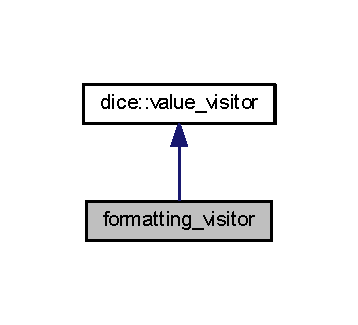
\includegraphics[width=172pt]{classformatting__visitor__inherit__graph}
\end{center}
\end{figure}


Collaboration diagram for formatting\+\_\+visitor\+:\nopagebreak
\begin{figure}[H]
\begin{center}
\leavevmode
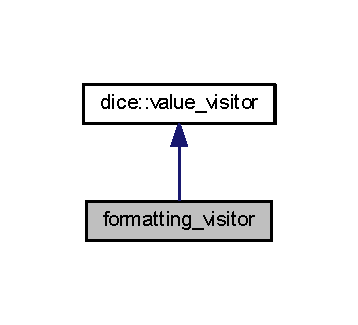
\includegraphics[width=172pt]{classformatting__visitor__coll__graph}
\end{center}
\end{figure}
\subsection*{Public Member Functions}
\begin{DoxyCompactItemize}
\item 
\mbox{\Hypertarget{classformatting__visitor_a12ae5e283e6bcfd8e065ff0dac3855d1}\label{classformatting__visitor_a12ae5e283e6bcfd8e065ff0dac3855d1}} 
void {\bfseries visit} (\mbox{\hyperlink{classdice_1_1typed__value}{dice\+::type\+\_\+int}} $\ast$value) override
\item 
\mbox{\Hypertarget{classformatting__visitor_a03c54a2e80425c1d484fdce7c6654015}\label{classformatting__visitor_a03c54a2e80425c1d484fdce7c6654015}} 
void {\bfseries visit} (\mbox{\hyperlink{classdice_1_1typed__value}{dice\+::type\+\_\+real}} $\ast$value) override
\item 
\mbox{\Hypertarget{classformatting__visitor_a76ba84428d8e146bfd501b5bb569a770}\label{classformatting__visitor_a76ba84428d8e146bfd501b5bb569a770}} 
void {\bfseries visit} (\mbox{\hyperlink{classdice_1_1typed__value}{dice\+::type\+\_\+rand\+\_\+var}} $\ast$value) override
\end{DoxyCompactItemize}


The documentation for this class was generated from the following file\+:\begin{DoxyCompactItemize}
\item 
C\+:/projects/dice/src/main.\+cpp\end{DoxyCompactItemize}

\hypertarget{classdice_1_1function__definition}{}\section{dice\+:\+:function\+\_\+definition Class Reference}
\label{classdice_1_1function__definition}\index{dice\+::function\+\_\+definition@{dice\+::function\+\_\+definition}}


Object representing a function callable from a dice expression.  




{\ttfamily \#include $<$functions.\+hpp$>$}

\subsection*{Public Types}
\begin{DoxyCompactItemize}
\item 
\mbox{\Hypertarget{classdice_1_1function__definition_aa70e7d16099e2eaf30cf4c6ffb58f7e3}\label{classdice_1_1function__definition_aa70e7d16099e2eaf30cf4c6ffb58f7e3}} 
using {\bfseries fn} = \mbox{\hyperlink{classdice_1_1execution__context}{execution\+\_\+context}}
\end{DoxyCompactItemize}
\subsection*{Public Member Functions}
\begin{DoxyCompactItemize}
\item 
\mbox{\hyperlink{classdice_1_1function__definition_a002ceae34d8dba6d5a83da97fad28c62}{function\+\_\+definition}} (fn\+::callable\+\_\+type callable)
\begin{DoxyCompactList}\small\item\em Create function without arguments. \end{DoxyCompactList}\item 
\mbox{\hyperlink{classdice_1_1function__definition_a8722346987d1cc191032dffb5e912f6f}{function\+\_\+definition}} (fn\+::callable\+\_\+type callable, std\+::vector$<$ \mbox{\hyperlink{value_8hpp_ab9af7d8ecc381e026ca4d07a745f23eb}{type\+\_\+id}} $>$ \&\&arg\+\_\+types)
\begin{DoxyCompactList}\small\item\em Create function with arguments. \end{DoxyCompactList}\item 
\mbox{\Hypertarget{classdice_1_1function__definition_a3992982ebfe549c336f118fef8d194ff}\label{classdice_1_1function__definition_a3992982ebfe549c336f118fef8d194ff}} 
{\bfseries function\+\_\+definition} (const \mbox{\hyperlink{classdice_1_1function__definition}{function\+\_\+definition}} \&)=delete
\item 
\mbox{\Hypertarget{classdice_1_1function__definition_a74d45bd0799e47a9553bf0956ee81b6e}\label{classdice_1_1function__definition_a74d45bd0799e47a9553bf0956ee81b6e}} 
void {\bfseries operator=} (const \mbox{\hyperlink{classdice_1_1function__definition}{function\+\_\+definition}} \&)=delete
\item 
\mbox{\Hypertarget{classdice_1_1function__definition_aa7ef0a9eaf695e23c8a54f8954e3535b}\label{classdice_1_1function__definition_aa7ef0a9eaf695e23c8a54f8954e3535b}} 
{\bfseries function\+\_\+definition} (\mbox{\hyperlink{classdice_1_1function__definition}{function\+\_\+definition}} \&\&)=default
\item 
\mbox{\Hypertarget{classdice_1_1function__definition_a7a06f9ea590076435ad36d0df6650aef}\label{classdice_1_1function__definition_a7a06f9ea590076435ad36d0df6650aef}} 
\mbox{\hyperlink{classdice_1_1function__definition}{function\+\_\+definition}} \& {\bfseries operator=} (\mbox{\hyperlink{classdice_1_1function__definition}{function\+\_\+definition}} \&\&)=default
\item 
fn\+::return\+\_\+type \mbox{\hyperlink{classdice_1_1function__definition_ae88e53c3dca93ccf845ecb894db7672b}{operator()}} (\mbox{\hyperlink{classdice_1_1execution__context}{fn\+::context\+\_\+type}} \&context) const
\begin{DoxyCompactList}\small\item\em Call this user function with given arguments. \end{DoxyCompactList}\item 
\mbox{\hyperlink{value_8hpp_ab9af7d8ecc381e026ca4d07a745f23eb}{type\+\_\+id}} \mbox{\hyperlink{classdice_1_1function__definition_a1aba35d197d5db50f229bc81f4f489d3}{arg\+\_\+type}} (std\+::size\+\_\+t index) const
\begin{DoxyCompactList}\small\item\em Get type of the ith argument. \end{DoxyCompactList}\item 
std\+::size\+\_\+t \mbox{\hyperlink{classdice_1_1function__definition_a5de84af8250e195aaf76bf84856d9aeb}{argc}} () const
\begin{DoxyCompactList}\small\item\em Get number of function arguments. \end{DoxyCompactList}\end{DoxyCompactItemize}


\subsection{Detailed Description}
Object representing a function callable from a dice expression. 

Example -\/ function metadata\+: 
\begin{DoxyCode}
function\_definition func\{ ..., \{ type\_id::integer, type\_id::real \} \};
assert(func.argc() == 2);
assert(func.arg\_type(0) == type\_id::integer);
assert(func.arg\_type(1) == type\_id::real);
\end{DoxyCode}


Example -\/ call function\+: 
\begin{DoxyCode}
std::vector<execution\_context::value\_type> args\{ 
     make<type\_int>(1), 
     make<type\_real>(3.1415) 
\};
execution\_context context\{ args.begin(), args.end() \};
func(context);
\end{DoxyCode}
 

\subsection{Constructor \& Destructor Documentation}
\mbox{\Hypertarget{classdice_1_1function__definition_a002ceae34d8dba6d5a83da97fad28c62}\label{classdice_1_1function__definition_a002ceae34d8dba6d5a83da97fad28c62}} 
\index{dice\+::function\+\_\+definition@{dice\+::function\+\_\+definition}!function\+\_\+definition@{function\+\_\+definition}}
\index{function\+\_\+definition@{function\+\_\+definition}!dice\+::function\+\_\+definition@{dice\+::function\+\_\+definition}}
\subsubsection{\texorpdfstring{function\+\_\+definition()}{function\_definition()}\hspace{0.1cm}{\footnotesize\ttfamily [1/2]}}
{\footnotesize\ttfamily dice\+::function\+\_\+definition\+::function\+\_\+definition (\begin{DoxyParamCaption}\item[{fn\+::callable\+\_\+type}]{callable }\end{DoxyParamCaption})\hspace{0.3cm}{\ttfamily [inline]}, {\ttfamily [explicit]}}



Create function without arguments. 


\begin{DoxyParams}{Parameters}
{\em callable} & function implementation. It takes execution\+\_\+context\+::value\+\_\+type type as an argument. it returns execution\+\_\+context\+::return\+\_\+type type. \\
\hline
\end{DoxyParams}
\mbox{\Hypertarget{classdice_1_1function__definition_a8722346987d1cc191032dffb5e912f6f}\label{classdice_1_1function__definition_a8722346987d1cc191032dffb5e912f6f}} 
\index{dice\+::function\+\_\+definition@{dice\+::function\+\_\+definition}!function\+\_\+definition@{function\+\_\+definition}}
\index{function\+\_\+definition@{function\+\_\+definition}!dice\+::function\+\_\+definition@{dice\+::function\+\_\+definition}}
\subsubsection{\texorpdfstring{function\+\_\+definition()}{function\_definition()}\hspace{0.1cm}{\footnotesize\ttfamily [2/2]}}
{\footnotesize\ttfamily dice\+::function\+\_\+definition\+::function\+\_\+definition (\begin{DoxyParamCaption}\item[{fn\+::callable\+\_\+type}]{callable,  }\item[{std\+::vector$<$ \mbox{\hyperlink{value_8hpp_ab9af7d8ecc381e026ca4d07a745f23eb}{type\+\_\+id}} $>$ \&\&}]{arg\+\_\+types }\end{DoxyParamCaption})\hspace{0.3cm}{\ttfamily [inline]}}



Create function with arguments. 


\begin{DoxyParams}{Parameters}
{\em callable} & function implementation. It takes execution\+\_\+context\+::value\+\_\+type type as an argument. It returns execution\+\_\+context\+::return\+\_\+type type. \\
\hline
{\em arg\+\_\+types} & vector of argument types of this function. \\
\hline
\end{DoxyParams}


\subsection{Member Function Documentation}
\mbox{\Hypertarget{classdice_1_1function__definition_a1aba35d197d5db50f229bc81f4f489d3}\label{classdice_1_1function__definition_a1aba35d197d5db50f229bc81f4f489d3}} 
\index{dice\+::function\+\_\+definition@{dice\+::function\+\_\+definition}!arg\+\_\+type@{arg\+\_\+type}}
\index{arg\+\_\+type@{arg\+\_\+type}!dice\+::function\+\_\+definition@{dice\+::function\+\_\+definition}}
\subsubsection{\texorpdfstring{arg\+\_\+type()}{arg\_type()}}
{\footnotesize\ttfamily \mbox{\hyperlink{value_8hpp_ab9af7d8ecc381e026ca4d07a745f23eb}{type\+\_\+id}} dice\+::function\+\_\+definition\+::arg\+\_\+type (\begin{DoxyParamCaption}\item[{std\+::size\+\_\+t}]{index }\end{DoxyParamCaption}) const\hspace{0.3cm}{\ttfamily [inline]}}



Get type of the ith argument. 


\begin{DoxyParams}{Parameters}
{\em index} & of an argument \\
\hline
\end{DoxyParams}
\begin{DoxyReturn}{Returns}
type of the argument 
\end{DoxyReturn}
\mbox{\Hypertarget{classdice_1_1function__definition_a5de84af8250e195aaf76bf84856d9aeb}\label{classdice_1_1function__definition_a5de84af8250e195aaf76bf84856d9aeb}} 
\index{dice\+::function\+\_\+definition@{dice\+::function\+\_\+definition}!argc@{argc}}
\index{argc@{argc}!dice\+::function\+\_\+definition@{dice\+::function\+\_\+definition}}
\subsubsection{\texorpdfstring{argc()}{argc()}}
{\footnotesize\ttfamily std\+::size\+\_\+t dice\+::function\+\_\+definition\+::argc (\begin{DoxyParamCaption}{ }\end{DoxyParamCaption}) const\hspace{0.3cm}{\ttfamily [inline]}}



Get number of function arguments. 

\begin{DoxyReturn}{Returns}
number of arguemtns of this function 
\end{DoxyReturn}
\mbox{\Hypertarget{classdice_1_1function__definition_ae88e53c3dca93ccf845ecb894db7672b}\label{classdice_1_1function__definition_ae88e53c3dca93ccf845ecb894db7672b}} 
\index{dice\+::function\+\_\+definition@{dice\+::function\+\_\+definition}!operator()@{operator()}}
\index{operator()@{operator()}!dice\+::function\+\_\+definition@{dice\+::function\+\_\+definition}}
\subsubsection{\texorpdfstring{operator()()}{operator()()}}
{\footnotesize\ttfamily fn\+::return\+\_\+type dice\+::function\+\_\+definition\+::operator() (\begin{DoxyParamCaption}\item[{\mbox{\hyperlink{classdice_1_1execution__context}{fn\+::context\+\_\+type}} \&}]{context }\end{DoxyParamCaption}) const\hspace{0.3cm}{\ttfamily [inline]}}



Call this user function with given arguments. 


\begin{DoxyParams}{Parameters}
{\em context} & of execution of this call\\
\hline
\end{DoxyParams}
\begin{DoxyReturn}{Returns}
result of the call 
\end{DoxyReturn}


The documentation for this class was generated from the following file\+:\begin{DoxyCompactItemize}
\item 
C\+:/projects/dice/src/functions.\+hpp\end{DoxyCompactItemize}

\hypertarget{structstd_1_1hash_3_01dice_1_1safe_3_01T_01_4_01_4}{}\section{std\+:\+:hash$<$ dice\+:\+:safe$<$ T $>$ $>$ Struct Template Reference}
\label{structstd_1_1hash_3_01dice_1_1safe_3_01T_01_4_01_4}\index{std\+::hash$<$ dice\+::safe$<$ T $>$ $>$@{std\+::hash$<$ dice\+::safe$<$ T $>$ $>$}}
\subsection*{Public Member Functions}
\begin{DoxyCompactItemize}
\item 
\mbox{\Hypertarget{structstd_1_1hash_3_01dice_1_1safe_3_01T_01_4_01_4_aa5c468b6494a69dbc2aabb873e068119}\label{structstd_1_1hash_3_01dice_1_1safe_3_01T_01_4_01_4_aa5c468b6494a69dbc2aabb873e068119}} 
std\+::size\+\_\+t {\bfseries operator()} (const \mbox{\hyperlink{safe_8hpp_acd796e346e2b746739435c4a2983edba}{dice\+::safe}}$<$ T $>$ \&value) const
\end{DoxyCompactItemize}
\subsection*{Public Attributes}
\begin{DoxyCompactItemize}
\item 
\mbox{\Hypertarget{structstd_1_1hash_3_01dice_1_1safe_3_01T_01_4_01_4_afdb7f9c99526bff85493fd38216a6225}\label{structstd_1_1hash_3_01dice_1_1safe_3_01T_01_4_01_4_afdb7f9c99526bff85493fd38216a6225}} 
std\+::hash$<$ T $>$ {\bfseries hasher}
\end{DoxyCompactItemize}


The documentation for this struct was generated from the following file\+:\begin{DoxyCompactItemize}
\item 
C\+:/projects/dice/src/\mbox{\hyperlink{safe_8hpp}{safe.\+hpp}}\end{DoxyCompactItemize}

\hypertarget{classdice_1_1lexer}{}\section{dice\+:\+:lexer$<$ Logger $>$ Class Template Reference}
\label{classdice_1_1lexer}\index{dice\+::lexer$<$ Logger $>$@{dice\+::lexer$<$ Logger $>$}}


Lexer of a dice script.  




{\ttfamily \#include $<$lexer.\+hpp$>$}

\subsection*{Public Member Functions}
\begin{DoxyCompactItemize}
\item 
\mbox{\Hypertarget{classdice_1_1lexer_a3bc4744741a0ecbcb5f967d338a7ba00}\label{classdice_1_1lexer_a3bc4744741a0ecbcb5f967d338a7ba00}} 
{\bfseries lexer} (std\+::istream $\ast$input, Logger $\ast$log)
\item 
\mbox{\Hypertarget{classdice_1_1lexer_af1a50cceede3c51fdb3c007df9df4c7f}\label{classdice_1_1lexer_af1a50cceede3c51fdb3c007df9df4c7f}} 
{\bfseries lexer} (const \mbox{\hyperlink{classdice_1_1lexer}{lexer}} \&)=delete
\item 
\mbox{\Hypertarget{classdice_1_1lexer_afb1a3f61435f8f0d25755f493b45c852}\label{classdice_1_1lexer_afb1a3f61435f8f0d25755f493b45c852}} 
void {\bfseries operator=} (const \mbox{\hyperlink{classdice_1_1lexer}{lexer}} \&)=delete
\item 
\mbox{\Hypertarget{classdice_1_1lexer_abd6e792ad9d6ad88e991544b14842e39}\label{classdice_1_1lexer_abd6e792ad9d6ad88e991544b14842e39}} 
{\bfseries lexer} (\mbox{\hyperlink{classdice_1_1lexer}{lexer}} \&\&)=default
\item 
\mbox{\Hypertarget{classdice_1_1lexer_a295deda298887957f8afb659a11ead00}\label{classdice_1_1lexer_a295deda298887957f8afb659a11ead00}} 
\mbox{\hyperlink{classdice_1_1lexer}{lexer}} \& {\bfseries operator=} (\mbox{\hyperlink{classdice_1_1lexer}{lexer}} \&\&)=default
\item 
\mbox{\hyperlink{structdice_1_1symbol}{symbol}} \mbox{\hyperlink{classdice_1_1lexer_a7dd396caa4bfcd3416569eb1be07ecdd}{read\+\_\+token}} ()
\begin{DoxyCompactList}\small\item\em Read token at current location. \end{DoxyCompactList}\item 
const \mbox{\hyperlink{structdice_1_1lexer__location}{lexer\+\_\+location}} \& \mbox{\hyperlink{classdice_1_1lexer_a1e62241846b4736d744fe9bb61385cc3}{location}} () const
\begin{DoxyCompactList}\small\item\em Return current location of the lexer in the input stream. \end{DoxyCompactList}\end{DoxyCompactItemize}


\subsection{Detailed Description}
\subsubsection*{template$<$typename Logger$>$\newline
class dice\+::lexer$<$ Logger $>$}

Lexer of a dice script. 


\begin{DoxyTemplParams}{Template Parameters}
{\em Logger} & the logger type \\
\hline
\end{DoxyTemplParams}


\subsection{Member Function Documentation}
\mbox{\Hypertarget{classdice_1_1lexer_a1e62241846b4736d744fe9bb61385cc3}\label{classdice_1_1lexer_a1e62241846b4736d744fe9bb61385cc3}} 
\index{dice\+::lexer@{dice\+::lexer}!location@{location}}
\index{location@{location}!dice\+::lexer@{dice\+::lexer}}
\subsubsection{\texorpdfstring{location()}{location()}}
{\footnotesize\ttfamily template$<$typename Logger $>$ \\
const \mbox{\hyperlink{structdice_1_1lexer__location}{lexer\+\_\+location}}\& \mbox{\hyperlink{classdice_1_1lexer}{dice\+::lexer}}$<$ Logger $>$\+::location (\begin{DoxyParamCaption}{ }\end{DoxyParamCaption}) const\hspace{0.3cm}{\ttfamily [inline]}}



Return current location of the lexer in the input stream. 

\begin{DoxyReturn}{Returns}
current location of the lexer 
\end{DoxyReturn}
\mbox{\Hypertarget{classdice_1_1lexer_a7dd396caa4bfcd3416569eb1be07ecdd}\label{classdice_1_1lexer_a7dd396caa4bfcd3416569eb1be07ecdd}} 
\index{dice\+::lexer@{dice\+::lexer}!read\+\_\+token@{read\+\_\+token}}
\index{read\+\_\+token@{read\+\_\+token}!dice\+::lexer@{dice\+::lexer}}
\subsubsection{\texorpdfstring{read\+\_\+token()}{read\_token()}}
{\footnotesize\ttfamily template$<$typename Logger $>$ \\
\mbox{\hyperlink{structdice_1_1symbol}{symbol}} \mbox{\hyperlink{classdice_1_1lexer}{dice\+::lexer}}$<$ Logger $>$\+::read\+\_\+token (\begin{DoxyParamCaption}{ }\end{DoxyParamCaption})\hspace{0.3cm}{\ttfamily [inline]}}



Read token at current location. 

Decode a sequance of characters as a token and advance in the input stream. Skip all whitespace characters after the token (that is location after calling read\+\_\+token points to the beginning of the next token).

All errors will be logged with given logger.

\begin{DoxyReturn}{Returns}
token at current position 
\end{DoxyReturn}


The documentation for this class was generated from the following file\+:\begin{DoxyCompactItemize}
\item 
C\+:/projects/dice/src/lexer.\+hpp\end{DoxyCompactItemize}

\hypertarget{structdice_1_1lexer__location}{}\section{dice\+:\+:lexer\+\_\+location Struct Reference}
\label{structdice_1_1lexer__location}\index{dice\+::lexer\+\_\+location@{dice\+::lexer\+\_\+location}}


Location in an input stream.  




{\ttfamily \#include $<$lexer.\+hpp$>$}

\subsection*{Public Member Functions}
\begin{DoxyCompactItemize}
\item 
\mbox{\Hypertarget{structdice_1_1lexer__location_aa77b6af01f59fe8aecbd3e23e930dbf9}\label{structdice_1_1lexer__location_aa77b6af01f59fe8aecbd3e23e930dbf9}} 
{\bfseries lexer\+\_\+location} (int line, int col)
\end{DoxyCompactItemize}
\subsection*{Public Attributes}
\begin{DoxyCompactItemize}
\item 
\mbox{\Hypertarget{structdice_1_1lexer__location_abdc889c92dc1661c08aa9790e6f64e2c}\label{structdice_1_1lexer__location_abdc889c92dc1661c08aa9790e6f64e2c}} 
int {\bfseries line} = 0
\item 
\mbox{\Hypertarget{structdice_1_1lexer__location_a978d43983b9ef3601bc7217f980650b3}\label{structdice_1_1lexer__location_a978d43983b9ef3601bc7217f980650b3}} 
int {\bfseries col} = 0
\end{DoxyCompactItemize}


\subsection{Detailed Description}
Location in an input stream. 

Line and column are numbered from 0. 

The documentation for this struct was generated from the following file\+:\begin{DoxyCompactItemize}
\item 
C\+:/projects/dice/src/lexer.\+hpp\end{DoxyCompactItemize}

\hypertarget{classdice_1_1logger}{}\section{dice\+:\+:logger Class Reference}
\label{classdice_1_1logger}\index{dice\+::logger@{dice\+::logger}}


This class prints all errors in given output stream.  




{\ttfamily \#include $<$logger.\+hpp$>$}

\subsection*{Public Member Functions}
\begin{DoxyCompactItemize}
\item 
\mbox{\hyperlink{classdice_1_1logger_af96ff92a37f7376d0e96b2e3a65a0f6c}{logger}} ()
\begin{DoxyCompactList}\small\item\em Use std\+::cerr as the output of the logger. \end{DoxyCompactList}\item 
\mbox{\hyperlink{classdice_1_1logger_a945c88b202299d0fa387ffa5fe1d7bb9}{logger}} (std\+::ostream $\ast$output, bool print\+\_\+just\+\_\+message=false)
\begin{DoxyCompactList}\small\item\em Use given output stream as the output of the logger. \end{DoxyCompactList}\item 
void \mbox{\hyperlink{classdice_1_1logger_a5fb04ac776c40a57cee18ceb4fbdae9e}{error}} (int line, int column, const std\+::string \&message)
\begin{DoxyCompactList}\small\item\em Add a new error log. \end{DoxyCompactList}\item 
bool \mbox{\hyperlink{classdice_1_1logger_a7323ce67ddcf4d61f33ae000ec0421ac}{empty}} () const
\begin{DoxyCompactList}\small\item\em Check whether there were some errors logged. \end{DoxyCompactList}\end{DoxyCompactItemize}


\subsection{Detailed Description}
This class prints all errors in given output stream. 

Example usage\+: 
\begin{DoxyCode}
\mbox{\hyperlink{classdice_1_1logger_af96ff92a37f7376d0e96b2e3a65a0f6c}{logger}} log\{ &std::cin \};
assert(log.empty());
log.error(0, 14, \textcolor{stringliteral}{"Critical error"});
assert(!log.empty());
\end{DoxyCode}
 

\subsection{Constructor \& Destructor Documentation}
\mbox{\Hypertarget{classdice_1_1logger_af96ff92a37f7376d0e96b2e3a65a0f6c}\label{classdice_1_1logger_af96ff92a37f7376d0e96b2e3a65a0f6c}} 
\index{dice\+::logger@{dice\+::logger}!logger@{logger}}
\index{logger@{logger}!dice\+::logger@{dice\+::logger}}
\subsubsection{\texorpdfstring{logger()}{logger()}\hspace{0.1cm}{\footnotesize\ttfamily [1/2]}}
{\footnotesize\ttfamily dice\+::logger\+::logger (\begin{DoxyParamCaption}{ }\end{DoxyParamCaption})}



Use std\+::cerr as the output of the logger. 

\mbox{\Hypertarget{classdice_1_1logger_a945c88b202299d0fa387ffa5fe1d7bb9}\label{classdice_1_1logger_a945c88b202299d0fa387ffa5fe1d7bb9}} 
\index{dice\+::logger@{dice\+::logger}!logger@{logger}}
\index{logger@{logger}!dice\+::logger@{dice\+::logger}}
\subsubsection{\texorpdfstring{logger()}{logger()}\hspace{0.1cm}{\footnotesize\ttfamily [2/2]}}
{\footnotesize\ttfamily dice\+::logger\+::logger (\begin{DoxyParamCaption}\item[{std\+::ostream $\ast$}]{output,  }\item[{bool}]{print\+\_\+just\+\_\+message = {\ttfamily false} }\end{DoxyParamCaption})\hspace{0.3cm}{\ttfamily [explicit]}}



Use given output stream as the output of the logger. 


\begin{DoxyParams}{Parameters}
{\em output} & pointer to an output stream \\
\hline
{\em print\+\_\+just\+\_\+message} & if true, the logger will only print unformated error message (no error location or message formatting) \\
\hline
\end{DoxyParams}


\subsection{Member Function Documentation}
\mbox{\Hypertarget{classdice_1_1logger_a7323ce67ddcf4d61f33ae000ec0421ac}\label{classdice_1_1logger_a7323ce67ddcf4d61f33ae000ec0421ac}} 
\index{dice\+::logger@{dice\+::logger}!empty@{empty}}
\index{empty@{empty}!dice\+::logger@{dice\+::logger}}
\subsubsection{\texorpdfstring{empty()}{empty()}}
{\footnotesize\ttfamily bool dice\+::logger\+::empty (\begin{DoxyParamCaption}{ }\end{DoxyParamCaption}) const}



Check whether there were some errors logged. 

\begin{DoxyReturn}{Returns}
true I\+FF there were no errors 
\end{DoxyReturn}
\mbox{\Hypertarget{classdice_1_1logger_a5fb04ac776c40a57cee18ceb4fbdae9e}\label{classdice_1_1logger_a5fb04ac776c40a57cee18ceb4fbdae9e}} 
\index{dice\+::logger@{dice\+::logger}!error@{error}}
\index{error@{error}!dice\+::logger@{dice\+::logger}}
\subsubsection{\texorpdfstring{error()}{error()}}
{\footnotesize\ttfamily void dice\+::logger\+::error (\begin{DoxyParamCaption}\item[{int}]{line,  }\item[{int}]{column,  }\item[{const std\+::string \&}]{message }\end{DoxyParamCaption})}



Add a new error log. 


\begin{DoxyParams}{Parameters}
{\em line} & of the input at which the error occured \\
\hline
{\em column} & in which the error occured\\
\hline
{\em message} & of the error \\
\hline
\end{DoxyParams}


The documentation for this class was generated from the following files\+:\begin{DoxyCompactItemize}
\item 
C\+:/projects/dice/src/logger.\+hpp\item 
C\+:/projects/dice/src/logger.\+cpp\end{DoxyCompactItemize}

\hypertarget{classdice_1_1nonterminal}{}\section{dice\+:\+:nonterminal$<$ type $>$ Class Template Reference}
\label{classdice_1_1nonterminal}\index{dice\+::nonterminal$<$ type $>$@{dice\+::nonterminal$<$ type $>$}}


The documentation for this class was generated from the following file\+:\begin{DoxyCompactItemize}
\item 
C\+:/projects/dice/src/parser.\+hpp\end{DoxyCompactItemize}

\hypertarget{classdice_1_1nonterminal_3_01nonterminal__type_1_1add_01_4}{}\section{dice\+:\+:nonterminal$<$ nonterminal\+\_\+type\+:\+:add $>$ Class Template Reference}
\label{classdice_1_1nonterminal_3_01nonterminal__type_1_1add_01_4}\index{dice\+::nonterminal$<$ nonterminal\+\_\+type\+::add $>$@{dice\+::nonterminal$<$ nonterminal\+\_\+type\+::add $>$}}
\subsection*{Static Public Attributes}
\begin{DoxyCompactItemize}
\item 
\mbox{\Hypertarget{classdice_1_1nonterminal_3_01nonterminal__type_1_1add_01_4_a3b40b9a88563652e016b15406f4fe7f7}\label{classdice_1_1nonterminal_3_01nonterminal__type_1_1add_01_4_a3b40b9a88563652e016b15406f4fe7f7}} 
static const char {\bfseries name} \mbox{[}$\,$\mbox{]}
\item 
\mbox{\Hypertarget{classdice_1_1nonterminal_3_01nonterminal__type_1_1add_01_4_adb8cb5488ce6c11ff3025419bafd9515}\label{classdice_1_1nonterminal_3_01nonterminal__type_1_1add_01_4_adb8cb5488ce6c11ff3025419bafd9515}} 
static const std\+::array$<$ \mbox{\hyperlink{symbols_8hpp_ab0295a855bb7eadc138abd6993af3aea}{symbol\+\_\+type}}, 5 $>$ {\bfseries first}
\item 
\mbox{\Hypertarget{classdice_1_1nonterminal_3_01nonterminal__type_1_1add_01_4_aa1cf8e132ca8cfa99eba81d526eae9c0}\label{classdice_1_1nonterminal_3_01nonterminal__type_1_1add_01_4_aa1cf8e132ca8cfa99eba81d526eae9c0}} 
static const std\+::array$<$ \mbox{\hyperlink{symbols_8hpp_ab0295a855bb7eadc138abd6993af3aea}{symbol\+\_\+type}}, 9 $>$ {\bfseries follow}
\end{DoxyCompactItemize}


The documentation for this class was generated from the following file\+:\begin{DoxyCompactItemize}
\item 
C\+:/projects/dice/src/parser.\+hpp\end{DoxyCompactItemize}

\hypertarget{classdice_1_1nonterminal_3_01nonterminal__type_1_1dice__roll_01_4}{}\section{dice\+:\+:nonterminal$<$ nonterminal\+\_\+type\+:\+:dice\+\_\+roll $>$ Class Template Reference}
\label{classdice_1_1nonterminal_3_01nonterminal__type_1_1dice__roll_01_4}\index{dice\+::nonterminal$<$ nonterminal\+\_\+type\+::dice\+\_\+roll $>$@{dice\+::nonterminal$<$ nonterminal\+\_\+type\+::dice\+\_\+roll $>$}}
\subsection*{Static Public Attributes}
\begin{DoxyCompactItemize}
\item 
\mbox{\Hypertarget{classdice_1_1nonterminal_3_01nonterminal__type_1_1dice__roll_01_4_a6aa8e87cfa2d56d0e52f12392cec493d}\label{classdice_1_1nonterminal_3_01nonterminal__type_1_1dice__roll_01_4_a6aa8e87cfa2d56d0e52f12392cec493d}} 
static const char {\bfseries name} \mbox{[}$\,$\mbox{]}
\item 
\mbox{\Hypertarget{classdice_1_1nonterminal_3_01nonterminal__type_1_1dice__roll_01_4_aa772f327b119c60a8482f8d55baac0bd}\label{classdice_1_1nonterminal_3_01nonterminal__type_1_1dice__roll_01_4_aa772f327b119c60a8482f8d55baac0bd}} 
static const std\+::array$<$ \mbox{\hyperlink{symbols_8hpp_ab0295a855bb7eadc138abd6993af3aea}{symbol\+\_\+type}}, 5 $>$ {\bfseries first}
\item 
\mbox{\Hypertarget{classdice_1_1nonterminal_3_01nonterminal__type_1_1dice__roll_01_4_ac8fdea83740eeec5db4ed5ef4955453e}\label{classdice_1_1nonterminal_3_01nonterminal__type_1_1dice__roll_01_4_ac8fdea83740eeec5db4ed5ef4955453e}} 
static const std\+::array$<$ \mbox{\hyperlink{symbols_8hpp_ab0295a855bb7eadc138abd6993af3aea}{symbol\+\_\+type}}, 12 $>$ {\bfseries follow}
\end{DoxyCompactItemize}


The documentation for this class was generated from the following file\+:\begin{DoxyCompactItemize}
\item 
C\+:/projects/dice/src/parser.\+hpp\end{DoxyCompactItemize}

\hypertarget{classdice_1_1nonterminal_3_01nonterminal__type_1_1expr_01_4}{}\section{dice\+:\+:nonterminal$<$ nonterminal\+\_\+type\+:\+:expr $>$ Class Template Reference}
\label{classdice_1_1nonterminal_3_01nonterminal__type_1_1expr_01_4}\index{dice\+::nonterminal$<$ nonterminal\+\_\+type\+::expr $>$@{dice\+::nonterminal$<$ nonterminal\+\_\+type\+::expr $>$}}
\subsection*{Static Public Attributes}
\begin{DoxyCompactItemize}
\item 
\mbox{\Hypertarget{classdice_1_1nonterminal_3_01nonterminal__type_1_1expr_01_4_ae305b2458e6b9b30cfd60101b9858c93}\label{classdice_1_1nonterminal_3_01nonterminal__type_1_1expr_01_4_ae305b2458e6b9b30cfd60101b9858c93}} 
static const char {\bfseries name} \mbox{[}$\,$\mbox{]}
\item 
\mbox{\Hypertarget{classdice_1_1nonterminal_3_01nonterminal__type_1_1expr_01_4_abae7eeaed72faff338531a172dc08588}\label{classdice_1_1nonterminal_3_01nonterminal__type_1_1expr_01_4_abae7eeaed72faff338531a172dc08588}} 
static const std\+::array$<$ \mbox{\hyperlink{symbols_8hpp_ab0295a855bb7eadc138abd6993af3aea}{symbol\+\_\+type}}, 5 $>$ {\bfseries first}
\item 
\mbox{\Hypertarget{classdice_1_1nonterminal_3_01nonterminal__type_1_1expr_01_4_a0b7fbfaed00ca33514b97cacbf0db4dc}\label{classdice_1_1nonterminal_3_01nonterminal__type_1_1expr_01_4_a0b7fbfaed00ca33514b97cacbf0db4dc}} 
static const std\+::array$<$ \mbox{\hyperlink{symbols_8hpp_ab0295a855bb7eadc138abd6993af3aea}{symbol\+\_\+type}}, 4 $>$ {\bfseries follow}
\end{DoxyCompactItemize}


The documentation for this class was generated from the following file\+:\begin{DoxyCompactItemize}
\item 
C\+:/projects/dice/src/parser.\+hpp\end{DoxyCompactItemize}

\hypertarget{classdice_1_1nonterminal_3_01nonterminal__type_1_1factor_01_4}{}\section{dice\+:\+:nonterminal$<$ nonterminal\+\_\+type\+:\+:factor $>$ Class Template Reference}
\label{classdice_1_1nonterminal_3_01nonterminal__type_1_1factor_01_4}\index{dice\+::nonterminal$<$ nonterminal\+\_\+type\+::factor $>$@{dice\+::nonterminal$<$ nonterminal\+\_\+type\+::factor $>$}}
\subsection*{Static Public Attributes}
\begin{DoxyCompactItemize}
\item 
\mbox{\Hypertarget{classdice_1_1nonterminal_3_01nonterminal__type_1_1factor_01_4_af194940c14f77c2883114c1764dc57bb}\label{classdice_1_1nonterminal_3_01nonterminal__type_1_1factor_01_4_af194940c14f77c2883114c1764dc57bb}} 
static const char {\bfseries name} \mbox{[}$\,$\mbox{]}
\item 
\mbox{\Hypertarget{classdice_1_1nonterminal_3_01nonterminal__type_1_1factor_01_4_a974be1eeeae580b9e6442340e02ef4a9}\label{classdice_1_1nonterminal_3_01nonterminal__type_1_1factor_01_4_a974be1eeeae580b9e6442340e02ef4a9}} 
static const std\+::array$<$ \mbox{\hyperlink{symbols_8hpp_ab0295a855bb7eadc138abd6993af3aea}{symbol\+\_\+type}}, 4 $>$ {\bfseries first}
\item 
\mbox{\Hypertarget{classdice_1_1nonterminal_3_01nonterminal__type_1_1factor_01_4_a4016566c1d20e2b8265be7e07568a660}\label{classdice_1_1nonterminal_3_01nonterminal__type_1_1factor_01_4_a4016566c1d20e2b8265be7e07568a660}} 
static const std\+::array$<$ \mbox{\hyperlink{symbols_8hpp_ab0295a855bb7eadc138abd6993af3aea}{symbol\+\_\+type}}, 12 $>$ {\bfseries follow}
\end{DoxyCompactItemize}


The documentation for this class was generated from the following file\+:\begin{DoxyCompactItemize}
\item 
C\+:/projects/dice/src/parser.\+hpp\end{DoxyCompactItemize}

\hypertarget{classdice_1_1nonterminal_3_01nonterminal__type_1_1mult_01_4}{}\section{dice\+:\+:nonterminal$<$ nonterminal\+\_\+type\+:\+:mult $>$ Class Template Reference}
\label{classdice_1_1nonterminal_3_01nonterminal__type_1_1mult_01_4}\index{dice\+::nonterminal$<$ nonterminal\+\_\+type\+::mult $>$@{dice\+::nonterminal$<$ nonterminal\+\_\+type\+::mult $>$}}
\subsection*{Static Public Attributes}
\begin{DoxyCompactItemize}
\item 
\mbox{\Hypertarget{classdice_1_1nonterminal_3_01nonterminal__type_1_1mult_01_4_a0cad6f35671701ccd566b4a704d57ff8}\label{classdice_1_1nonterminal_3_01nonterminal__type_1_1mult_01_4_a0cad6f35671701ccd566b4a704d57ff8}} 
static const char {\bfseries name} \mbox{[}$\,$\mbox{]}
\item 
\mbox{\Hypertarget{classdice_1_1nonterminal_3_01nonterminal__type_1_1mult_01_4_a0aad0ceeb53c4b94ba8e819a30596539}\label{classdice_1_1nonterminal_3_01nonterminal__type_1_1mult_01_4_a0aad0ceeb53c4b94ba8e819a30596539}} 
static const std\+::array$<$ \mbox{\hyperlink{symbols_8hpp_ab0295a855bb7eadc138abd6993af3aea}{symbol\+\_\+type}}, 5 $>$ {\bfseries first}
\item 
\mbox{\Hypertarget{classdice_1_1nonterminal_3_01nonterminal__type_1_1mult_01_4_a21b3828061f359b340f16d494c83f790}\label{classdice_1_1nonterminal_3_01nonterminal__type_1_1mult_01_4_a21b3828061f359b340f16d494c83f790}} 
static const std\+::array$<$ \mbox{\hyperlink{symbols_8hpp_ab0295a855bb7eadc138abd6993af3aea}{symbol\+\_\+type}}, 11 $>$ {\bfseries follow}
\end{DoxyCompactItemize}


The documentation for this class was generated from the following file\+:\begin{DoxyCompactItemize}
\item 
C\+:/projects/dice/src/parser.\+hpp\end{DoxyCompactItemize}

\hypertarget{classdice_1_1nonterminal_3_01nonterminal__type_1_1param__list_01_4}{}\section{dice\+:\+:nonterminal$<$ nonterminal\+\_\+type\+:\+:param\+\_\+list $>$ Class Template Reference}
\label{classdice_1_1nonterminal_3_01nonterminal__type_1_1param__list_01_4}\index{dice\+::nonterminal$<$ nonterminal\+\_\+type\+::param\+\_\+list $>$@{dice\+::nonterminal$<$ nonterminal\+\_\+type\+::param\+\_\+list $>$}}
\subsection*{Static Public Attributes}
\begin{DoxyCompactItemize}
\item 
\mbox{\Hypertarget{classdice_1_1nonterminal_3_01nonterminal__type_1_1param__list_01_4_a8244706e04083632e32f04450c1df6ab}\label{classdice_1_1nonterminal_3_01nonterminal__type_1_1param__list_01_4_a8244706e04083632e32f04450c1df6ab}} 
static const char {\bfseries name} \mbox{[}$\,$\mbox{]}
\item 
\mbox{\Hypertarget{classdice_1_1nonterminal_3_01nonterminal__type_1_1param__list_01_4_a2883b61ba83ba16df71aea6810d72f27}\label{classdice_1_1nonterminal_3_01nonterminal__type_1_1param__list_01_4_a2883b61ba83ba16df71aea6810d72f27}} 
static const std\+::array$<$ \mbox{\hyperlink{symbols_8hpp_ab0295a855bb7eadc138abd6993af3aea}{symbol\+\_\+type}}, 6 $>$ {\bfseries first}
\item 
\mbox{\Hypertarget{classdice_1_1nonterminal_3_01nonterminal__type_1_1param__list_01_4_a9c561cf8eb727314cd97cfe9e9fbd511}\label{classdice_1_1nonterminal_3_01nonterminal__type_1_1param__list_01_4_a9c561cf8eb727314cd97cfe9e9fbd511}} 
static const std\+::array$<$ \mbox{\hyperlink{symbols_8hpp_ab0295a855bb7eadc138abd6993af3aea}{symbol\+\_\+type}}, 2 $>$ {\bfseries follow}
\end{DoxyCompactItemize}


The documentation for this class was generated from the following file\+:\begin{DoxyCompactItemize}
\item 
C\+:/projects/dice/src/parser.\+hpp\end{DoxyCompactItemize}

\hypertarget{classdice_1_1nonterminal_3_01nonterminal__type_1_1stmt_01_4}{}\section{dice\+:\+:nonterminal$<$ nonterminal\+\_\+type\+:\+:stmt $>$ Class Template Reference}
\label{classdice_1_1nonterminal_3_01nonterminal__type_1_1stmt_01_4}\index{dice\+::nonterminal$<$ nonterminal\+\_\+type\+::stmt $>$@{dice\+::nonterminal$<$ nonterminal\+\_\+type\+::stmt $>$}}
\subsection*{Static Public Attributes}
\begin{DoxyCompactItemize}
\item 
\mbox{\Hypertarget{classdice_1_1nonterminal_3_01nonterminal__type_1_1stmt_01_4_ae91b9e3364c1b4bc7cd52f7e91d40bd6}\label{classdice_1_1nonterminal_3_01nonterminal__type_1_1stmt_01_4_ae91b9e3364c1b4bc7cd52f7e91d40bd6}} 
static const char {\bfseries name} \mbox{[}$\,$\mbox{]}
\item 
\mbox{\Hypertarget{classdice_1_1nonterminal_3_01nonterminal__type_1_1stmt_01_4_a9c3ac7c54b8cc103ccf86a43dbbee66d}\label{classdice_1_1nonterminal_3_01nonterminal__type_1_1stmt_01_4_a9c3ac7c54b8cc103ccf86a43dbbee66d}} 
static const std\+::array$<$ \mbox{\hyperlink{symbols_8hpp_ab0295a855bb7eadc138abd6993af3aea}{symbol\+\_\+type}}, 6 $>$ {\bfseries first}
\item 
\mbox{\Hypertarget{classdice_1_1nonterminal_3_01nonterminal__type_1_1stmt_01_4_ae9618f437a5b6528d0f8c3f1ca2951b7}\label{classdice_1_1nonterminal_3_01nonterminal__type_1_1stmt_01_4_ae9618f437a5b6528d0f8c3f1ca2951b7}} 
static const std\+::array$<$ \mbox{\hyperlink{symbols_8hpp_ab0295a855bb7eadc138abd6993af3aea}{symbol\+\_\+type}}, 2 $>$ {\bfseries follow}
\end{DoxyCompactItemize}


The documentation for this class was generated from the following file\+:\begin{DoxyCompactItemize}
\item 
C\+:/projects/dice/src/parser.\+hpp\end{DoxyCompactItemize}

\hypertarget{classdice_1_1nonterminal_3_01nonterminal__type_1_1stmts_01_4}{}\section{dice\+:\+:nonterminal$<$ nonterminal\+\_\+type\+:\+:stmts $>$ Class Template Reference}
\label{classdice_1_1nonterminal_3_01nonterminal__type_1_1stmts_01_4}\index{dice\+::nonterminal$<$ nonterminal\+\_\+type\+::stmts $>$@{dice\+::nonterminal$<$ nonterminal\+\_\+type\+::stmts $>$}}
\subsection*{Static Public Attributes}
\begin{DoxyCompactItemize}
\item 
\mbox{\Hypertarget{classdice_1_1nonterminal_3_01nonterminal__type_1_1stmts_01_4_aad94bdf80aaead384b8ca5f77e664e63}\label{classdice_1_1nonterminal_3_01nonterminal__type_1_1stmts_01_4_aad94bdf80aaead384b8ca5f77e664e63}} 
static const char {\bfseries name} \mbox{[}$\,$\mbox{]}
\item 
\mbox{\Hypertarget{classdice_1_1nonterminal_3_01nonterminal__type_1_1stmts_01_4_adba6a09bc0831f44300d70cba3c70f7a}\label{classdice_1_1nonterminal_3_01nonterminal__type_1_1stmts_01_4_adba6a09bc0831f44300d70cba3c70f7a}} 
static const std\+::array$<$ \mbox{\hyperlink{symbols_8hpp_ab0295a855bb7eadc138abd6993af3aea}{symbol\+\_\+type}}, 7 $>$ {\bfseries first}
\item 
\mbox{\Hypertarget{classdice_1_1nonterminal_3_01nonterminal__type_1_1stmts_01_4_ab181d697c8e58118cc564aa7c8bb3a33}\label{classdice_1_1nonterminal_3_01nonterminal__type_1_1stmts_01_4_ab181d697c8e58118cc564aa7c8bb3a33}} 
static const std\+::array$<$ \mbox{\hyperlink{symbols_8hpp_ab0295a855bb7eadc138abd6993af3aea}{symbol\+\_\+type}}, 1 $>$ {\bfseries follow}
\end{DoxyCompactItemize}


The documentation for this class was generated from the following file\+:\begin{DoxyCompactItemize}
\item 
C\+:/projects/dice/src/parser.\+hpp\end{DoxyCompactItemize}

\hypertarget{classstd_1_1numeric__limits_3_01dice_1_1safe_3_01T_01_4_01_4}{}\section{std\+:\+:numeric\+\_\+limits$<$ dice\+:\+:safe$<$ T $>$ $>$ Class Template Reference}
\label{classstd_1_1numeric__limits_3_01dice_1_1safe_3_01T_01_4_01_4}\index{std\+::numeric\+\_\+limits$<$ dice\+::safe$<$ T $>$ $>$@{std\+::numeric\+\_\+limits$<$ dice\+::safe$<$ T $>$ $>$}}
\subsection*{Static Public Member Functions}
\begin{DoxyCompactItemize}
\item 
\mbox{\Hypertarget{classstd_1_1numeric__limits_3_01dice_1_1safe_3_01T_01_4_01_4_a97cfb8c3de73ffd4df9b5220e8b9475c}\label{classstd_1_1numeric__limits_3_01dice_1_1safe_3_01T_01_4_01_4_a97cfb8c3de73ffd4df9b5220e8b9475c}} 
static constexpr \mbox{\hyperlink{safe_8hpp_acd796e346e2b746739435c4a2983edba}{dice\+::safe}}$<$ T $>$ {\bfseries lowest} ()
\item 
\mbox{\Hypertarget{classstd_1_1numeric__limits_3_01dice_1_1safe_3_01T_01_4_01_4_a6e2df63214d969fe081684f30e853906}\label{classstd_1_1numeric__limits_3_01dice_1_1safe_3_01T_01_4_01_4_a6e2df63214d969fe081684f30e853906}} 
static constexpr \mbox{\hyperlink{safe_8hpp_acd796e346e2b746739435c4a2983edba}{dice\+::safe}}$<$ T $>$ {\bfseries min} ()
\item 
\mbox{\Hypertarget{classstd_1_1numeric__limits_3_01dice_1_1safe_3_01T_01_4_01_4_a7aa0e628742910d99c2638068b24d194}\label{classstd_1_1numeric__limits_3_01dice_1_1safe_3_01T_01_4_01_4_a7aa0e628742910d99c2638068b24d194}} 
static constexpr \mbox{\hyperlink{safe_8hpp_acd796e346e2b746739435c4a2983edba}{dice\+::safe}}$<$ T $>$ {\bfseries max} ()
\item 
\mbox{\Hypertarget{classstd_1_1numeric__limits_3_01dice_1_1safe_3_01T_01_4_01_4_a9813a0ef58e72d30557426f38e3686e7}\label{classstd_1_1numeric__limits_3_01dice_1_1safe_3_01T_01_4_01_4_a9813a0ef58e72d30557426f38e3686e7}} 
static constexpr \mbox{\hyperlink{safe_8hpp_acd796e346e2b746739435c4a2983edba}{dice\+::safe}}$<$ T $>$ {\bfseries epsilon} ()
\item 
\mbox{\Hypertarget{classstd_1_1numeric__limits_3_01dice_1_1safe_3_01T_01_4_01_4_a094f8771a105ddc4ab7da6ce6701c915}\label{classstd_1_1numeric__limits_3_01dice_1_1safe_3_01T_01_4_01_4_a094f8771a105ddc4ab7da6ce6701c915}} 
static constexpr auto {\bfseries round\+\_\+error} ()
\item 
\mbox{\Hypertarget{classstd_1_1numeric__limits_3_01dice_1_1safe_3_01T_01_4_01_4_a40f299cea90ad8cca4d4fcb764b805e1}\label{classstd_1_1numeric__limits_3_01dice_1_1safe_3_01T_01_4_01_4_a40f299cea90ad8cca4d4fcb764b805e1}} 
static constexpr \mbox{\hyperlink{safe_8hpp_acd796e346e2b746739435c4a2983edba}{dice\+::safe}}$<$ T $>$ {\bfseries infinity} ()
\item 
\mbox{\Hypertarget{classstd_1_1numeric__limits_3_01dice_1_1safe_3_01T_01_4_01_4_ab62c220dd32fee521a4a67cb9ed6a1fa}\label{classstd_1_1numeric__limits_3_01dice_1_1safe_3_01T_01_4_01_4_ab62c220dd32fee521a4a67cb9ed6a1fa}} 
static constexpr \mbox{\hyperlink{safe_8hpp_acd796e346e2b746739435c4a2983edba}{dice\+::safe}}$<$ T $>$ {\bfseries quiet\+\_\+\+NaN} ()
\item 
\mbox{\Hypertarget{classstd_1_1numeric__limits_3_01dice_1_1safe_3_01T_01_4_01_4_aa2c71ac62a31619ff4f2366a8e7911e7}\label{classstd_1_1numeric__limits_3_01dice_1_1safe_3_01T_01_4_01_4_aa2c71ac62a31619ff4f2366a8e7911e7}} 
static constexpr \mbox{\hyperlink{safe_8hpp_acd796e346e2b746739435c4a2983edba}{dice\+::safe}}$<$ T $>$ {\bfseries signaling\+\_\+\+NaN} ()
\item 
\mbox{\Hypertarget{classstd_1_1numeric__limits_3_01dice_1_1safe_3_01T_01_4_01_4_af2f6893ac8a8057b40c4afb513a6a83d}\label{classstd_1_1numeric__limits_3_01dice_1_1safe_3_01T_01_4_01_4_af2f6893ac8a8057b40c4afb513a6a83d}} 
static constexpr \mbox{\hyperlink{safe_8hpp_acd796e346e2b746739435c4a2983edba}{dice\+::safe}}$<$ T $>$ {\bfseries denorm\+\_\+min} ()
\end{DoxyCompactItemize}
\subsection*{Static Public Attributes}
\begin{DoxyCompactItemize}
\item 
\mbox{\Hypertarget{classstd_1_1numeric__limits_3_01dice_1_1safe_3_01T_01_4_01_4_a05fa9aff3d883d02d24f53fddcf05e02}\label{classstd_1_1numeric__limits_3_01dice_1_1safe_3_01T_01_4_01_4_a05fa9aff3d883d02d24f53fddcf05e02}} 
static constexpr auto {\bfseries is\+\_\+specialized} = numeric\+\_\+limits$<$T$>$\+::is\+\_\+specialized
\item 
\mbox{\Hypertarget{classstd_1_1numeric__limits_3_01dice_1_1safe_3_01T_01_4_01_4_a0d2a811355deff07c6aeeb7774f4e0dd}\label{classstd_1_1numeric__limits_3_01dice_1_1safe_3_01T_01_4_01_4_a0d2a811355deff07c6aeeb7774f4e0dd}} 
static constexpr auto {\bfseries is\+\_\+signed} = numeric\+\_\+limits$<$T$>$\+::is\+\_\+signed
\item 
\mbox{\Hypertarget{classstd_1_1numeric__limits_3_01dice_1_1safe_3_01T_01_4_01_4_a45936b19185cab03efe5ed9fbb94aa7d}\label{classstd_1_1numeric__limits_3_01dice_1_1safe_3_01T_01_4_01_4_a45936b19185cab03efe5ed9fbb94aa7d}} 
static constexpr auto {\bfseries is\+\_\+integer} = numeric\+\_\+limits$<$T$>$\+::is\+\_\+integer
\item 
\mbox{\Hypertarget{classstd_1_1numeric__limits_3_01dice_1_1safe_3_01T_01_4_01_4_a73b5a099f772068f7fe232832697b58d}\label{classstd_1_1numeric__limits_3_01dice_1_1safe_3_01T_01_4_01_4_a73b5a099f772068f7fe232832697b58d}} 
static constexpr auto {\bfseries is\+\_\+exact} = numeric\+\_\+limits$<$T$>$\+::is\+\_\+exact
\item 
\mbox{\Hypertarget{classstd_1_1numeric__limits_3_01dice_1_1safe_3_01T_01_4_01_4_a75fd47ce7c1c6c5f25ad6d1bf5346fae}\label{classstd_1_1numeric__limits_3_01dice_1_1safe_3_01T_01_4_01_4_a75fd47ce7c1c6c5f25ad6d1bf5346fae}} 
static constexpr auto {\bfseries has\+\_\+infinity} = numeric\+\_\+limits$<$T$>$\+::has\+\_\+infinity
\item 
\mbox{\Hypertarget{classstd_1_1numeric__limits_3_01dice_1_1safe_3_01T_01_4_01_4_a5b8368d034ed57c893049fc6f736b5e4}\label{classstd_1_1numeric__limits_3_01dice_1_1safe_3_01T_01_4_01_4_a5b8368d034ed57c893049fc6f736b5e4}} 
static constexpr auto {\bfseries has\+\_\+quiet\+\_\+\+NaN} = numeric\+\_\+limits$<$T$>$\+::has\+\_\+quiet\+\_\+\+NaN
\item 
\mbox{\Hypertarget{classstd_1_1numeric__limits_3_01dice_1_1safe_3_01T_01_4_01_4_a12ab5a95fd3f33554d085309d75d2759}\label{classstd_1_1numeric__limits_3_01dice_1_1safe_3_01T_01_4_01_4_a12ab5a95fd3f33554d085309d75d2759}} 
static constexpr auto {\bfseries has\+\_\+signaling\+\_\+\+NaN} = numeric\+\_\+limits$<$T$>$\+::has\+\_\+signaling\+\_\+\+NaN
\item 
\mbox{\Hypertarget{classstd_1_1numeric__limits_3_01dice_1_1safe_3_01T_01_4_01_4_aeb43cfd8d14912d6269cb508a876bc61}\label{classstd_1_1numeric__limits_3_01dice_1_1safe_3_01T_01_4_01_4_aeb43cfd8d14912d6269cb508a876bc61}} 
static constexpr auto {\bfseries has\+\_\+denorm} = numeric\+\_\+limits$<$T$>$\+::has\+\_\+denorm
\item 
\mbox{\Hypertarget{classstd_1_1numeric__limits_3_01dice_1_1safe_3_01T_01_4_01_4_a58b032007c89e09ea5778377f19d94e8}\label{classstd_1_1numeric__limits_3_01dice_1_1safe_3_01T_01_4_01_4_a58b032007c89e09ea5778377f19d94e8}} 
static constexpr auto {\bfseries has\+\_\+denorm\+\_\+loss} = numeric\+\_\+limits$<$T$>$\+::has\+\_\+denorm\+\_\+loss
\item 
\mbox{\Hypertarget{classstd_1_1numeric__limits_3_01dice_1_1safe_3_01T_01_4_01_4_a5c22fdc463f0b8b9718106a7ac8f29c4}\label{classstd_1_1numeric__limits_3_01dice_1_1safe_3_01T_01_4_01_4_a5c22fdc463f0b8b9718106a7ac8f29c4}} 
static constexpr auto {\bfseries round\+\_\+style} = numeric\+\_\+limits$<$T$>$\+::round\+\_\+style
\item 
\mbox{\Hypertarget{classstd_1_1numeric__limits_3_01dice_1_1safe_3_01T_01_4_01_4_a4a23ba13b179a61b8d74c20117454040}\label{classstd_1_1numeric__limits_3_01dice_1_1safe_3_01T_01_4_01_4_a4a23ba13b179a61b8d74c20117454040}} 
static constexpr auto {\bfseries is\+\_\+iec559} = numeric\+\_\+limits$<$T$>$\+::is\+\_\+iec559
\item 
\mbox{\Hypertarget{classstd_1_1numeric__limits_3_01dice_1_1safe_3_01T_01_4_01_4_a3604a7c398f6ec782380fedb43209930}\label{classstd_1_1numeric__limits_3_01dice_1_1safe_3_01T_01_4_01_4_a3604a7c398f6ec782380fedb43209930}} 
static constexpr auto {\bfseries is\+\_\+bounded} = numeric\+\_\+limits$<$T$>$\+::is\+\_\+bounded
\item 
\mbox{\Hypertarget{classstd_1_1numeric__limits_3_01dice_1_1safe_3_01T_01_4_01_4_aef120043edfd12361252b03ac4c7a458}\label{classstd_1_1numeric__limits_3_01dice_1_1safe_3_01T_01_4_01_4_aef120043edfd12361252b03ac4c7a458}} 
static constexpr auto {\bfseries is\+\_\+modulo} = numeric\+\_\+limits$<$T$>$\+::is\+\_\+modulo
\item 
\mbox{\Hypertarget{classstd_1_1numeric__limits_3_01dice_1_1safe_3_01T_01_4_01_4_a7d62b138650e6cafaffd6a6413f69eae}\label{classstd_1_1numeric__limits_3_01dice_1_1safe_3_01T_01_4_01_4_a7d62b138650e6cafaffd6a6413f69eae}} 
static constexpr auto {\bfseries digits} = numeric\+\_\+limits$<$T$>$\+::digits
\item 
\mbox{\Hypertarget{classstd_1_1numeric__limits_3_01dice_1_1safe_3_01T_01_4_01_4_acbf18f49af3595e02c0cde3cb6b9d2f0}\label{classstd_1_1numeric__limits_3_01dice_1_1safe_3_01T_01_4_01_4_acbf18f49af3595e02c0cde3cb6b9d2f0}} 
static constexpr auto {\bfseries digits10} = numeric\+\_\+limits$<$T$>$\+::digits10
\item 
\mbox{\Hypertarget{classstd_1_1numeric__limits_3_01dice_1_1safe_3_01T_01_4_01_4_a2d9255f64505f657301b2f609db98c22}\label{classstd_1_1numeric__limits_3_01dice_1_1safe_3_01T_01_4_01_4_a2d9255f64505f657301b2f609db98c22}} 
static constexpr auto {\bfseries max\+\_\+digits10} = numeric\+\_\+limits$<$T$>$\+::max\+\_\+digits10
\item 
\mbox{\Hypertarget{classstd_1_1numeric__limits_3_01dice_1_1safe_3_01T_01_4_01_4_a99bf58f5a834db2086ef3f94e0fe822d}\label{classstd_1_1numeric__limits_3_01dice_1_1safe_3_01T_01_4_01_4_a99bf58f5a834db2086ef3f94e0fe822d}} 
static constexpr auto {\bfseries radix} = numeric\+\_\+limits$<$T$>$\+::radix
\item 
\mbox{\Hypertarget{classstd_1_1numeric__limits_3_01dice_1_1safe_3_01T_01_4_01_4_ad06799577c289324ceebcf7cc6dd9305}\label{classstd_1_1numeric__limits_3_01dice_1_1safe_3_01T_01_4_01_4_ad06799577c289324ceebcf7cc6dd9305}} 
static constexpr auto {\bfseries min\+\_\+exponent} = numeric\+\_\+limits$<$T$>$\+::min\+\_\+exponent
\item 
\mbox{\Hypertarget{classstd_1_1numeric__limits_3_01dice_1_1safe_3_01T_01_4_01_4_aaa4ad38b271f77d90761bc4bf5f8a2c1}\label{classstd_1_1numeric__limits_3_01dice_1_1safe_3_01T_01_4_01_4_aaa4ad38b271f77d90761bc4bf5f8a2c1}} 
static constexpr auto {\bfseries min\+\_\+exponent10} = numeric\+\_\+limits$<$T$>$\+::min\+\_\+exponent10
\item 
\mbox{\Hypertarget{classstd_1_1numeric__limits_3_01dice_1_1safe_3_01T_01_4_01_4_aa472b775571085cc9f3f7f5c4c12b73a}\label{classstd_1_1numeric__limits_3_01dice_1_1safe_3_01T_01_4_01_4_aa472b775571085cc9f3f7f5c4c12b73a}} 
static constexpr auto {\bfseries max\+\_\+exponent} = numeric\+\_\+limits$<$T$>$\+::max\+\_\+exponent
\item 
\mbox{\Hypertarget{classstd_1_1numeric__limits_3_01dice_1_1safe_3_01T_01_4_01_4_a96e8d7765ca27a230ff4b4eda1d83de9}\label{classstd_1_1numeric__limits_3_01dice_1_1safe_3_01T_01_4_01_4_a96e8d7765ca27a230ff4b4eda1d83de9}} 
static constexpr auto {\bfseries max\+\_\+exponent10} = numeric\+\_\+limits$<$T$>$\+::max\+\_\+exponent10
\item 
\mbox{\Hypertarget{classstd_1_1numeric__limits_3_01dice_1_1safe_3_01T_01_4_01_4_a363ca17b4ef8f955dbd563cb27937bb5}\label{classstd_1_1numeric__limits_3_01dice_1_1safe_3_01T_01_4_01_4_a363ca17b4ef8f955dbd563cb27937bb5}} 
static constexpr auto {\bfseries traps} = numeric\+\_\+limits$<$T$>$\+::traps
\item 
\mbox{\Hypertarget{classstd_1_1numeric__limits_3_01dice_1_1safe_3_01T_01_4_01_4_a8eb808e3678ca8fee5567a1addd96409}\label{classstd_1_1numeric__limits_3_01dice_1_1safe_3_01T_01_4_01_4_a8eb808e3678ca8fee5567a1addd96409}} 
static constexpr auto {\bfseries tinyness\+\_\+before} = numeric\+\_\+limits$<$T$>$\+::tinyness\+\_\+before
\end{DoxyCompactItemize}


The documentation for this class was generated from the following file\+:\begin{DoxyCompactItemize}
\item 
C\+:/projects/dice/src/\mbox{\hyperlink{safe_8hpp}{safe.\+hpp}}\end{DoxyCompactItemize}

\hypertarget{structoptions}{}\section{options Struct Reference}
\label{structoptions}\index{options@{options}}
\subsection*{Public Member Functions}
\begin{DoxyCompactItemize}
\item 
\mbox{\Hypertarget{structoptions_ab376d0aaddda72a964ce52343a998108}\label{structoptions_ab376d0aaddda72a964ce52343a998108}} 
{\bfseries options} (int argc, char $\ast$$\ast$argv)
\end{DoxyCompactItemize}
\subsection*{Public Attributes}
\begin{DoxyCompactItemize}
\item 
\mbox{\Hypertarget{structoptions_a9f001831f97e3c6efb3b1fe0180c6c2e}\label{structoptions_a9f001831f97e3c6efb3b1fe0180c6c2e}} 
std\+::vector$<$ std\+::string $>$ {\bfseries args}
\item 
\mbox{\Hypertarget{structoptions_aab9db55300fd148286188044ae96a41a}\label{structoptions_aab9db55300fd148286188044ae96a41a}} 
std\+::istream $\ast$ {\bfseries input}
\item 
\mbox{\Hypertarget{structoptions_a3c67beda9f93c75f6815b24f0d660e2a}\label{structoptions_a3c67beda9f93c75f6815b24f0d660e2a}} 
std\+::string {\bfseries input\+\_\+name}
\end{DoxyCompactItemize}


The documentation for this struct was generated from the following file\+:\begin{DoxyCompactItemize}
\item 
C\+:/projects/dice/src/main.\+cpp\end{DoxyCompactItemize}

\hypertarget{classdice_1_1parser}{}\section{dice\+:\+:parser$<$ Lexer, Logger, Interpreter $>$ Class Template Reference}
\label{classdice_1_1parser}\index{dice\+::parser$<$ Lexer, Logger, Interpreter $>$@{dice\+::parser$<$ Lexer, Logger, Interpreter $>$}}


Dice expression parser.  




{\ttfamily \#include $<$parser.\+hpp$>$}

\subsection*{Public Types}
\begin{DoxyCompactItemize}
\item 
\mbox{\Hypertarget{classdice_1_1parser_ad550d010318819123ef5a028322df8eb}\label{classdice_1_1parser_ad550d010318819123ef5a028322df8eb}} 
using \mbox{\hyperlink{classdice_1_1parser_ad550d010318819123ef5a028322df8eb}{attr\+\_\+type}} = typename Interpreter\+::value\+\_\+type
\begin{DoxyCompactList}\small\item\em Type of attributes of nonterminals. \end{DoxyCompactList}\end{DoxyCompactItemize}
\subsection*{Public Member Functions}
\begin{DoxyCompactItemize}
\item 
\mbox{\Hypertarget{classdice_1_1parser_a09510972db249f96cc49f1bb60cde597}\label{classdice_1_1parser_a09510972db249f96cc49f1bb60cde597}} 
{\bfseries parser} (Lexer $\ast$reader, Logger $\ast$log, Interpreter $\ast$inter)
\item 
auto \mbox{\hyperlink{classdice_1_1parser_a9166865af1db0974b2b372885bcc1501}{parse}} ()
\begin{DoxyCompactList}\small\item\em Parse expression provided by the lexer. \end{DoxyCompactList}\end{DoxyCompactItemize}


\subsection{Detailed Description}
\subsubsection*{template$<$typename Lexer, typename Logger, typename Interpreter$>$\newline
class dice\+::parser$<$ Lexer, Logger, Interpreter $>$}

Dice expression parser. 


\begin{DoxyTemplParams}{Template Parameters}
{\em Lexer} & the lexer type \\
\hline
{\em Logger} & the logger type \\
\hline
{\em Interpreter} & the \mbox{\hyperlink{classdice_1_1direct__interpreter}{direct\+\_\+interpreter}} type\\
\hline
\end{DoxyTemplParams}
\begin{DoxyAttention}{Attention}
It is possible to use custom types of lexer, logger or interpreter but it is recommended to use the default implementations of these types. Other types are used mainly for testing. 
\end{DoxyAttention}


\subsection{Member Function Documentation}
\mbox{\Hypertarget{classdice_1_1parser_a9166865af1db0974b2b372885bcc1501}\label{classdice_1_1parser_a9166865af1db0974b2b372885bcc1501}} 
\index{dice\+::parser@{dice\+::parser}!parse@{parse}}
\index{parse@{parse}!dice\+::parser@{dice\+::parser}}
\subsubsection{\texorpdfstring{parse()}{parse()}}
{\footnotesize\ttfamily template$<$typename Lexer , typename Logger , typename Interpreter $>$ \\
auto \mbox{\hyperlink{classdice_1_1parser}{dice\+::parser}}$<$ Lexer, Logger, Interpreter $>$\+::parse (\begin{DoxyParamCaption}{ }\end{DoxyParamCaption})\hspace{0.3cm}{\ttfamily [inline]}}



Parse expression provided by the lexer. 

Operators are left associative unless stated otherwise.

List of operators (from lowest to highest precedence)\+:
\begin{DoxyEnumerate}
\item = (assignment, non-\/associative)
\item $<$, $<$=, !=, ==, $>$=, $>$, in (relational operators, non-\/assosiative)
\item + (add), -\/ (subtract)
\item $\ast$ (multiply), / (divide)
\item -\/ (unary minus)
\item D$\vert$d (roll dice)
\end{DoxyEnumerate}

\begin{DoxyReturn}{Returns}
computed values 
\end{DoxyReturn}


The documentation for this class was generated from the following file\+:\begin{DoxyCompactItemize}
\item 
C\+:/projects/dice/src/parser.\+hpp\end{DoxyCompactItemize}

\hypertarget{classdice_1_1random__variable}{}\section{dice\+:\+:random\+\_\+variable$<$ Value\+Type, Probability\+Type $>$ Class Template Reference}
\label{classdice_1_1random__variable}\index{dice\+::random\+\_\+variable$<$ Value\+Type, Probability\+Type $>$@{dice\+::random\+\_\+variable$<$ Value\+Type, Probability\+Type $>$}}


Discrete random variable.  




{\ttfamily \#include $<$random\+\_\+variable.\+hpp$>$}

\subsection*{Public Types}
\begin{DoxyCompactItemize}
\item 
\mbox{\Hypertarget{classdice_1_1random__variable_ac9c699272072661cfddd880bd7bdf81b}\label{classdice_1_1random__variable_ac9c699272072661cfddd880bd7bdf81b}} 
using {\bfseries value\+\_\+type} = Value\+Type
\item 
\mbox{\Hypertarget{classdice_1_1random__variable_a38b4f4b7d42d5d5a6b9688bf03fab469}\label{classdice_1_1random__variable_a38b4f4b7d42d5d5a6b9688bf03fab469}} 
using {\bfseries probability\+\_\+type} = Probability\+Type
\item 
\mbox{\Hypertarget{classdice_1_1random__variable_abb6c151c9168391112bd1fc279f1984f}\label{classdice_1_1random__variable_abb6c151c9168391112bd1fc279f1984f}} 
using {\bfseries frequency\+\_\+list} = std\+::vector$<$ std\+::pair$<$ value\+\_\+type, std\+::size\+\_\+t $>$ $>$
\item 
\mbox{\Hypertarget{classdice_1_1random__variable_ab17dc25c146a0673d2b7aa14c997b2d6}\label{classdice_1_1random__variable_ab17dc25c146a0673d2b7aa14c997b2d6}} 
using {\bfseries probability\+\_\+list} = std\+::vector$<$ std\+::pair$<$ value\+\_\+type, probability\+\_\+type $>$ $>$
\end{DoxyCompactItemize}
\subsection*{Public Member Functions}
\begin{DoxyCompactItemize}
\item 
\mbox{\hyperlink{classdice_1_1random__variable_a7cf5a4706aebdb1d8d1fd362491df895}{random\+\_\+variable}} ()
\begin{DoxyCompactList}\small\item\em Create an impossible event. \end{DoxyCompactList}\item 
\mbox{\hyperlink{classdice_1_1random__variable_a50f56529bf017dbdc074f98ac6b9ac55}{random\+\_\+variable}} (\mbox{\hyperlink{classdice_1_1constant__tag}{constant\+\_\+tag}}, value\+\_\+type value)
\begin{DoxyCompactList}\small\item\em Create a constant. \end{DoxyCompactList}\item 
\mbox{\hyperlink{classdice_1_1random__variable_a96f7d3bfb204d1b213c1e004132492ee}{random\+\_\+variable}} (\mbox{\hyperlink{classdice_1_1bernoulli__tag}{bernoulli\+\_\+tag}}, probability\+\_\+type success\+\_\+prob)
\begin{DoxyCompactList}\small\item\em Create a bernoulli distribution. \end{DoxyCompactList}\item 
\mbox{\hyperlink{classdice_1_1random__variable_ae60bac2f1326a03ced717a4f0ff12513}{random\+\_\+variable}} (const frequency\+\_\+list \&list)
\begin{DoxyCompactList}\small\item\em Compute probabilities from list of value frequencies. \end{DoxyCompactList}\item 
\mbox{\Hypertarget{classdice_1_1random__variable_acf84e1446bdebc2be61df6dddf23926f}\label{classdice_1_1random__variable_acf84e1446bdebc2be61df6dddf23926f}} 
{\bfseries random\+\_\+variable} (const \mbox{\hyperlink{classdice_1_1random__variable}{random\+\_\+variable}} \&)=default
\item 
\mbox{\Hypertarget{classdice_1_1random__variable_a08f007500cac0eec18ec07b117be8662}\label{classdice_1_1random__variable_a08f007500cac0eec18ec07b117be8662}} 
\mbox{\hyperlink{classdice_1_1random__variable}{random\+\_\+variable}} \& {\bfseries operator=} (const \mbox{\hyperlink{classdice_1_1random__variable}{random\+\_\+variable}} \&)=default
\item 
\mbox{\Hypertarget{classdice_1_1random__variable_adfe32efb1c2f20260374a28078ed9b1f}\label{classdice_1_1random__variable_adfe32efb1c2f20260374a28078ed9b1f}} 
{\bfseries random\+\_\+variable} (\mbox{\hyperlink{classdice_1_1random__variable}{random\+\_\+variable}} \&\&)=default
\item 
\mbox{\Hypertarget{classdice_1_1random__variable_ad234b4fd5bb4422dcbd2e0b38ca95851}\label{classdice_1_1random__variable_ad234b4fd5bb4422dcbd2e0b38ca95851}} 
\mbox{\hyperlink{classdice_1_1random__variable}{random\+\_\+variable}} \& {\bfseries operator=} (\mbox{\hyperlink{classdice_1_1random__variable}{random\+\_\+variable}} \&\&)=default
\item 
bool \mbox{\hyperlink{classdice_1_1random__variable_a42d682610d251d5305dd349a71a023eb}{is\+\_\+constant}} () const
\begin{DoxyCompactList}\small\item\em Check whether this is a constant. \end{DoxyCompactList}\item 
auto \mbox{\hyperlink{classdice_1_1random__variable_a1cf78d3c3fa4b13d85215b873a50be5f}{max\+\_\+value}} () const
\begin{DoxyCompactList}\small\item\em Find maximal value in the variable\textquotesingle{}s range. \end{DoxyCompactList}\item 
auto \mbox{\hyperlink{classdice_1_1random__variable_ab926693f2773202c8fce755d4664052f}{min\+\_\+value}} () const
\begin{DoxyCompactList}\small\item\em Find minimal value in the variable\textquotesingle{}s range. \end{DoxyCompactList}\item 
auto \mbox{\hyperlink{classdice_1_1random__variable_a210faa1d7ac3aa393804d87f828ca91c}{expected\+\_\+value}} () const
\begin{DoxyCompactList}\small\item\em Compute expected value of this random variable. \end{DoxyCompactList}\item 
auto \mbox{\hyperlink{classdice_1_1random__variable_ae709a9985d1e722629fc13c26f405e61}{variance}} () const
\begin{DoxyCompactList}\small\item\em Compute variance of this random variable. \end{DoxyCompactList}\item 
auto \mbox{\hyperlink{classdice_1_1random__variable_ae72311eea3b8ad6c66893c2af3489d74}{deviation}} () const
\begin{DoxyCompactList}\small\item\em Calculate standard deviation of this random variable. \end{DoxyCompactList}\item 
auto \mbox{\hyperlink{classdice_1_1random__variable_aa1c5beebc469a8cc51906fd0b48ef5b1}{quantile}} (probability\+\_\+type \mbox{\hyperlink{classdice_1_1random__variable_a0759c25151ebb5618e2ff0ecbb91c80d}{probability}}) const
\begin{DoxyCompactList}\small\item\em Compute quantile of this random variable. \end{DoxyCompactList}\item 
auto \mbox{\hyperlink{classdice_1_1random__variable_a559e5f26fcd39e1f68b22681aab90664}{random\+\_\+value}} (probability\+\_\+type \mbox{\hyperlink{classdice_1_1random__variable_a0759c25151ebb5618e2ff0ecbb91c80d}{probability}}) const
\begin{DoxyCompactList}\small\item\em Return first value s.\+t. \end{DoxyCompactList}\item 
{\footnotesize template$<$typename T $>$ }\\\mbox{\hyperlink{classdice_1_1random__variable}{random\+\_\+variable}} \mbox{\hyperlink{classdice_1_1random__variable_a20c851091e966593c053252fb76f390e}{in}} (const T \&lower\+\_\+bound, const T \&upper\+\_\+bound) const
\begin{DoxyCompactList}\small\item\em Calculate indicator that X (this r.\+v.) is in given interval. \end{DoxyCompactList}\item 
auto \mbox{\hyperlink{classdice_1_1random__variable_a125e2b252af1eb4edd04011f81f080cf}{operator+}} (const \mbox{\hyperlink{classdice_1_1random__variable}{random\+\_\+variable}} \&other) const
\begin{DoxyCompactList}\small\item\em Compute distribution of X + Y (X is this random variable). \end{DoxyCompactList}\item 
auto \mbox{\hyperlink{classdice_1_1random__variable_a40ad720c40cb4467dbb2b735512b279c}{operator-\/}} (const \mbox{\hyperlink{classdice_1_1random__variable}{random\+\_\+variable}} \&other) const
\begin{DoxyCompactList}\small\item\em Compute distribution of X -\/ Y (X is this random variable). \end{DoxyCompactList}\item 
auto \mbox{\hyperlink{classdice_1_1random__variable_ac420c3a819add2d6115dfe5071f40b8e}{operator$\ast$}} (const \mbox{\hyperlink{classdice_1_1random__variable}{random\+\_\+variable}} \&other) const
\begin{DoxyCompactList}\small\item\em Compute distribution of X $\ast$ Y (X is this random variable). \end{DoxyCompactList}\item 
auto \mbox{\hyperlink{classdice_1_1random__variable_a52896f8ba19758fc240d6e8f51b650e7}{operator/}} (const \mbox{\hyperlink{classdice_1_1random__variable}{random\+\_\+variable}} \&other) const
\begin{DoxyCompactList}\small\item\em Compute distribution of integer division X / Y. \end{DoxyCompactList}\item 
auto \mbox{\hyperlink{classdice_1_1random__variable_a8447981f77852b91874f1f888dae50ac}{less\+\_\+than}} (const \mbox{\hyperlink{classdice_1_1random__variable}{random\+\_\+variable}} \&other) const
\begin{DoxyCompactList}\small\item\em Compute indicator of X $<$ Y (X is this random variable). \end{DoxyCompactList}\item 
auto \mbox{\hyperlink{classdice_1_1random__variable_ac384c7a722412306ea7af080ceb8a8c5}{less\+\_\+than\+\_\+or\+\_\+equal}} (const \mbox{\hyperlink{classdice_1_1random__variable}{random\+\_\+variable}} \&other) const
\begin{DoxyCompactList}\small\item\em Compute indicator of X $<$= Y (X is this random variable). \end{DoxyCompactList}\item 
auto \mbox{\hyperlink{classdice_1_1random__variable_ac66bb2ec2b0d9a67029a3a9381d02d61}{equal}} (const \mbox{\hyperlink{classdice_1_1random__variable}{random\+\_\+variable}} \&other) const
\begin{DoxyCompactList}\small\item\em Compute indicator of X = Y (X is this random variable). \end{DoxyCompactList}\item 
auto \mbox{\hyperlink{classdice_1_1random__variable_aeeabefcda0c3599eba97b98fab245021}{not\+\_\+equal}} (const \mbox{\hyperlink{classdice_1_1random__variable}{random\+\_\+variable}} \&other) const
\begin{DoxyCompactList}\small\item\em Compute indicator of X != Y (X is this random variable). \end{DoxyCompactList}\item 
auto \mbox{\hyperlink{classdice_1_1random__variable_abeb43cf9343eb0f26418b71f04a3b350}{greater\+\_\+than}} (const \mbox{\hyperlink{classdice_1_1random__variable}{random\+\_\+variable}} \&other) const
\begin{DoxyCompactList}\small\item\em Compute indicator of X $>$ Y (X is this random variable). \end{DoxyCompactList}\item 
auto \mbox{\hyperlink{classdice_1_1random__variable_a067075bcd32f952f4eadcd7a888038b5}{greater\+\_\+than\+\_\+or\+\_\+equal}} (const \mbox{\hyperlink{classdice_1_1random__variable}{random\+\_\+variable}} \&other) const
\begin{DoxyCompactList}\small\item\em Compute indicator of X $>$= Y (X is this random variable). \end{DoxyCompactList}\item 
auto \mbox{\hyperlink{classdice_1_1random__variable_a5900675092ca3ca0ea387628ed64624f}{operator-\/}} () const
\begin{DoxyCompactList}\small\item\em Compute negation of this random variable (-\/X) \end{DoxyCompactList}\item 
{\footnotesize template$<$typename Predicate $>$ }\\auto \mbox{\hyperlink{classdice_1_1random__variable_a79723edbb8e79a914f7b5ea37a13ed9a}{restrict}} (Predicate include) const
\begin{DoxyCompactList}\small\item\em Compute restriction of the range of this random variable. \end{DoxyCompactList}\item 
{\footnotesize template$<$typename Combination\+Function $>$ }\\auto \mbox{\hyperlink{classdice_1_1random__variable_a6aa92a82cfccdefe467410ec8e0d4dc7}{combine}} (const \mbox{\hyperlink{classdice_1_1random__variable}{random\+\_\+variable}} \&other, Combination\+Function combination) const
\begin{DoxyCompactList}\small\item\em Create a random variable that is a function of this variable X and the other variable Y. \end{DoxyCompactList}\item 
auto \mbox{\hyperlink{classdice_1_1random__variable_a0759c25151ebb5618e2ff0ecbb91c80d}{probability}} (const value\+\_\+type \&value) const
\begin{DoxyCompactList}\small\item\em Find the probability of given value. \end{DoxyCompactList}\item 
auto \mbox{\hyperlink{classdice_1_1random__variable_a60637ec353c3cd3046017d54824f1fd8}{size}} () const
\begin{DoxyCompactList}\small\item\em Return number of values in variable\textquotesingle{}s range. \end{DoxyCompactList}\item 
auto \mbox{\hyperlink{classdice_1_1random__variable_ad65ca036dd0c61483c888579b2d912fa}{begin}} () const
\begin{DoxyCompactList}\small\item\em First iterator of the (value, probaiblity) pair collection. \end{DoxyCompactList}\item 
auto \mbox{\hyperlink{classdice_1_1random__variable_a82f50939d82419d9f86901b6997ca8fe}{end}} () const
\begin{DoxyCompactList}\small\item\em Last iterator of the (value, probability) pair collection. \end{DoxyCompactList}\item 
bool \mbox{\hyperlink{classdice_1_1random__variable_a113037d3c11921f1ba1227a838781d3e}{empty}} () const
\begin{DoxyCompactList}\small\item\em Check whether there are any values with non-\/zero probability. \end{DoxyCompactList}\item 
bool \mbox{\hyperlink{classdice_1_1random__variable_abe0ae85dfb81c7f5b7c921db588eda17}{operator==}} (const \mbox{\hyperlink{classdice_1_1random__variable}{random\+\_\+variable}} \&other) const
\begin{DoxyCompactList}\small\item\em Chek whether this variable is equal to some other variable. \end{DoxyCompactList}\item 
\mbox{\Hypertarget{classdice_1_1random__variable_a46dbbc3797032825e095a658ff18d3ec}\label{classdice_1_1random__variable_a46dbbc3797032825e095a658ff18d3ec}} 
bool {\bfseries operator!=} (const \mbox{\hyperlink{classdice_1_1random__variable}{random\+\_\+variable}} \&other) const
\end{DoxyCompactItemize}
\subsection*{Friends}
\begin{DoxyCompactItemize}
\item 
\mbox{\Hypertarget{classdice_1_1random__variable_a576b2a57ac76cbde31cb0826a5cd1d6f}\label{classdice_1_1random__variable_a576b2a57ac76cbde31cb0826a5cd1d6f}} 
class {\bfseries decomposition$<$ Value\+Type, Probability\+Type $>$}
\item 
auto \mbox{\hyperlink{classdice_1_1random__variable_a1ee237915048ab90f60508a75ba39c40}{roll}} (const \mbox{\hyperlink{classdice_1_1random__variable}{random\+\_\+variable}} \&num\+\_\+dice, const \mbox{\hyperlink{classdice_1_1random__variable}{random\+\_\+variable}} \&num\+\_\+faces)
\begin{DoxyCompactList}\small\item\em Create a random variable Z = XdY. \end{DoxyCompactList}\end{DoxyCompactItemize}


\subsection{Detailed Description}
\subsubsection*{template$<$typename Value\+Type, typename Probability\+Type$>$\newline
class dice\+::random\+\_\+variable$<$ Value\+Type, Probability\+Type $>$}

Discrete random variable. 


\begin{DoxyTemplParams}{Template Parameters}
{\em Value\+Type} & type of a value of this variable. Requirements\+:
\begin{DoxyItemize}
\item std\+::numeric\+\_\+limits specialization
\item std\+::hash specialization
\item std\+::max, std\+::min specialization
\item convertible to Probability\+Type 
\end{DoxyItemize}\\
\hline
{\em Probability\+Type} & type of probability (rational number in \mbox{[}0, 1\mbox{]})\\
\hline
\end{DoxyTemplParams}
The Value\+Type is used as a key in a hash table. Probability\+Type is a value in this hash table. Probabilities of values sum up to 1.

This type is immutable. All public methods and functions which modify a variable return a new random variable. 

\subsection{Constructor \& Destructor Documentation}
\mbox{\Hypertarget{classdice_1_1random__variable_a7cf5a4706aebdb1d8d1fd362491df895}\label{classdice_1_1random__variable_a7cf5a4706aebdb1d8d1fd362491df895}} 
\index{dice\+::random\+\_\+variable@{dice\+::random\+\_\+variable}!random\+\_\+variable@{random\+\_\+variable}}
\index{random\+\_\+variable@{random\+\_\+variable}!dice\+::random\+\_\+variable@{dice\+::random\+\_\+variable}}
\subsubsection{\texorpdfstring{random\+\_\+variable()}{random\_variable()}\hspace{0.1cm}{\footnotesize\ttfamily [1/4]}}
{\footnotesize\ttfamily template$<$typename Value\+Type , typename Probability\+Type $>$ \\
\mbox{\hyperlink{classdice_1_1random__variable}{dice\+::random\+\_\+variable}}$<$ Value\+Type, Probability\+Type $>$\+::\mbox{\hyperlink{classdice_1_1random__variable}{random\+\_\+variable}} (\begin{DoxyParamCaption}{ }\end{DoxyParamCaption})\hspace{0.3cm}{\ttfamily [inline]}}



Create an impossible event. 

\mbox{\Hypertarget{classdice_1_1random__variable_a50f56529bf017dbdc074f98ac6b9ac55}\label{classdice_1_1random__variable_a50f56529bf017dbdc074f98ac6b9ac55}} 
\index{dice\+::random\+\_\+variable@{dice\+::random\+\_\+variable}!random\+\_\+variable@{random\+\_\+variable}}
\index{random\+\_\+variable@{random\+\_\+variable}!dice\+::random\+\_\+variable@{dice\+::random\+\_\+variable}}
\subsubsection{\texorpdfstring{random\+\_\+variable()}{random\_variable()}\hspace{0.1cm}{\footnotesize\ttfamily [2/4]}}
{\footnotesize\ttfamily template$<$typename Value\+Type , typename Probability\+Type $>$ \\
\mbox{\hyperlink{classdice_1_1random__variable}{dice\+::random\+\_\+variable}}$<$ Value\+Type, Probability\+Type $>$\+::\mbox{\hyperlink{classdice_1_1random__variable}{random\+\_\+variable}} (\begin{DoxyParamCaption}\item[{\mbox{\hyperlink{classdice_1_1constant__tag}{constant\+\_\+tag}}}]{,  }\item[{value\+\_\+type}]{value }\end{DoxyParamCaption})\hspace{0.3cm}{\ttfamily [inline]}}



Create a constant. 


\begin{DoxyParams}{Parameters}
{\em value} & of the constant \\
\hline
\end{DoxyParams}
\mbox{\Hypertarget{classdice_1_1random__variable_a96f7d3bfb204d1b213c1e004132492ee}\label{classdice_1_1random__variable_a96f7d3bfb204d1b213c1e004132492ee}} 
\index{dice\+::random\+\_\+variable@{dice\+::random\+\_\+variable}!random\+\_\+variable@{random\+\_\+variable}}
\index{random\+\_\+variable@{random\+\_\+variable}!dice\+::random\+\_\+variable@{dice\+::random\+\_\+variable}}
\subsubsection{\texorpdfstring{random\+\_\+variable()}{random\_variable()}\hspace{0.1cm}{\footnotesize\ttfamily [3/4]}}
{\footnotesize\ttfamily template$<$typename Value\+Type , typename Probability\+Type $>$ \\
\mbox{\hyperlink{classdice_1_1random__variable}{dice\+::random\+\_\+variable}}$<$ Value\+Type, Probability\+Type $>$\+::\mbox{\hyperlink{classdice_1_1random__variable}{random\+\_\+variable}} (\begin{DoxyParamCaption}\item[{\mbox{\hyperlink{classdice_1_1bernoulli__tag}{bernoulli\+\_\+tag}}}]{,  }\item[{probability\+\_\+type}]{success\+\_\+prob }\end{DoxyParamCaption})\hspace{0.3cm}{\ttfamily [inline]}}



Create a bernoulli distribution. 


\begin{DoxyParams}{Parameters}
{\em success\+\_\+prob} & probability of success If this is 0 or 1, the variable will be constant. \\
\hline
\end{DoxyParams}
\mbox{\Hypertarget{classdice_1_1random__variable_ae60bac2f1326a03ced717a4f0ff12513}\label{classdice_1_1random__variable_ae60bac2f1326a03ced717a4f0ff12513}} 
\index{dice\+::random\+\_\+variable@{dice\+::random\+\_\+variable}!random\+\_\+variable@{random\+\_\+variable}}
\index{random\+\_\+variable@{random\+\_\+variable}!dice\+::random\+\_\+variable@{dice\+::random\+\_\+variable}}
\subsubsection{\texorpdfstring{random\+\_\+variable()}{random\_variable()}\hspace{0.1cm}{\footnotesize\ttfamily [4/4]}}
{\footnotesize\ttfamily template$<$typename Value\+Type , typename Probability\+Type $>$ \\
\mbox{\hyperlink{classdice_1_1random__variable}{dice\+::random\+\_\+variable}}$<$ Value\+Type, Probability\+Type $>$\+::\mbox{\hyperlink{classdice_1_1random__variable}{random\+\_\+variable}} (\begin{DoxyParamCaption}\item[{const frequency\+\_\+list \&}]{list }\end{DoxyParamCaption})\hspace{0.3cm}{\ttfamily [inline]}, {\ttfamily [explicit]}}



Compute probabilities from list of value frequencies. 


\begin{DoxyParams}{Parameters}
{\em list} & of (value, frequency) pairs (values can repeat) \\
\hline
\end{DoxyParams}


\subsection{Member Function Documentation}
\mbox{\Hypertarget{classdice_1_1random__variable_ad65ca036dd0c61483c888579b2d912fa}\label{classdice_1_1random__variable_ad65ca036dd0c61483c888579b2d912fa}} 
\index{dice\+::random\+\_\+variable@{dice\+::random\+\_\+variable}!begin@{begin}}
\index{begin@{begin}!dice\+::random\+\_\+variable@{dice\+::random\+\_\+variable}}
\subsubsection{\texorpdfstring{begin()}{begin()}}
{\footnotesize\ttfamily template$<$typename Value\+Type , typename Probability\+Type $>$ \\
auto \mbox{\hyperlink{classdice_1_1random__variable}{dice\+::random\+\_\+variable}}$<$ Value\+Type, Probability\+Type $>$\+::begin (\begin{DoxyParamCaption}{ }\end{DoxyParamCaption}) const\hspace{0.3cm}{\ttfamily [inline]}}



First iterator of the (value, probaiblity) pair collection. 

\begin{DoxyReturn}{Returns}
iterator pointing to the first value 
\end{DoxyReturn}
\mbox{\Hypertarget{classdice_1_1random__variable_a6aa92a82cfccdefe467410ec8e0d4dc7}\label{classdice_1_1random__variable_a6aa92a82cfccdefe467410ec8e0d4dc7}} 
\index{dice\+::random\+\_\+variable@{dice\+::random\+\_\+variable}!combine@{combine}}
\index{combine@{combine}!dice\+::random\+\_\+variable@{dice\+::random\+\_\+variable}}
\subsubsection{\texorpdfstring{combine()}{combine()}}
{\footnotesize\ttfamily template$<$typename Value\+Type , typename Probability\+Type $>$ \\
template$<$typename Combination\+Function $>$ \\
auto \mbox{\hyperlink{classdice_1_1random__variable}{dice\+::random\+\_\+variable}}$<$ Value\+Type, Probability\+Type $>$\+::combine (\begin{DoxyParamCaption}\item[{const \mbox{\hyperlink{classdice_1_1random__variable}{random\+\_\+variable}}$<$ Value\+Type, Probability\+Type $>$ \&}]{other,  }\item[{Combination\+Function}]{combination }\end{DoxyParamCaption}) const\hspace{0.3cm}{\ttfamily [inline]}}



Create a random variable that is a function of this variable X and the other variable Y. 


\begin{DoxyTemplParams}{Template Parameters}
{\em Combination\+Function} & It takes value from X (Value\+Type), value from Y (Value\+Type) and returns their combination (Value\+Type).\\
\hline
\end{DoxyTemplParams}

\begin{DoxyParams}{Parameters}
{\em other} & random variable Y (independent of X) \\
\hline
{\em combination} & function of X and Y\\
\hline
\end{DoxyParams}
\begin{DoxyReturn}{Returns}
a new random variable that is a function of X and Y 
\end{DoxyReturn}
\mbox{\Hypertarget{classdice_1_1random__variable_ae72311eea3b8ad6c66893c2af3489d74}\label{classdice_1_1random__variable_ae72311eea3b8ad6c66893c2af3489d74}} 
\index{dice\+::random\+\_\+variable@{dice\+::random\+\_\+variable}!deviation@{deviation}}
\index{deviation@{deviation}!dice\+::random\+\_\+variable@{dice\+::random\+\_\+variable}}
\subsubsection{\texorpdfstring{deviation()}{deviation()}}
{\footnotesize\ttfamily template$<$typename Value\+Type , typename Probability\+Type $>$ \\
auto \mbox{\hyperlink{classdice_1_1random__variable}{dice\+::random\+\_\+variable}}$<$ Value\+Type, Probability\+Type $>$\+::deviation (\begin{DoxyParamCaption}{ }\end{DoxyParamCaption}) const\hspace{0.3cm}{\ttfamily [inline]}}



Calculate standard deviation of this random variable. 

\begin{DoxyReturn}{Returns}
standard deviation (square root or variance) 
\end{DoxyReturn}
\mbox{\Hypertarget{classdice_1_1random__variable_a113037d3c11921f1ba1227a838781d3e}\label{classdice_1_1random__variable_a113037d3c11921f1ba1227a838781d3e}} 
\index{dice\+::random\+\_\+variable@{dice\+::random\+\_\+variable}!empty@{empty}}
\index{empty@{empty}!dice\+::random\+\_\+variable@{dice\+::random\+\_\+variable}}
\subsubsection{\texorpdfstring{empty()}{empty()}}
{\footnotesize\ttfamily template$<$typename Value\+Type , typename Probability\+Type $>$ \\
bool \mbox{\hyperlink{classdice_1_1random__variable}{dice\+::random\+\_\+variable}}$<$ Value\+Type, Probability\+Type $>$\+::empty (\begin{DoxyParamCaption}{ }\end{DoxyParamCaption}) const\hspace{0.3cm}{\ttfamily [inline]}}



Check whether there are any values with non-\/zero probability. 

\begin{DoxyReturn}{Returns}
true iff there is at least 1 value with non-\/zero probability 
\end{DoxyReturn}
\mbox{\Hypertarget{classdice_1_1random__variable_a82f50939d82419d9f86901b6997ca8fe}\label{classdice_1_1random__variable_a82f50939d82419d9f86901b6997ca8fe}} 
\index{dice\+::random\+\_\+variable@{dice\+::random\+\_\+variable}!end@{end}}
\index{end@{end}!dice\+::random\+\_\+variable@{dice\+::random\+\_\+variable}}
\subsubsection{\texorpdfstring{end()}{end()}}
{\footnotesize\ttfamily template$<$typename Value\+Type , typename Probability\+Type $>$ \\
auto \mbox{\hyperlink{classdice_1_1random__variable}{dice\+::random\+\_\+variable}}$<$ Value\+Type, Probability\+Type $>$\+::end (\begin{DoxyParamCaption}{ }\end{DoxyParamCaption}) const\hspace{0.3cm}{\ttfamily [inline]}}



Last iterator of the (value, probability) pair collection. 

\begin{DoxyReturn}{Returns}
iterator pointing past the last value 
\end{DoxyReturn}
\mbox{\Hypertarget{classdice_1_1random__variable_ac66bb2ec2b0d9a67029a3a9381d02d61}\label{classdice_1_1random__variable_ac66bb2ec2b0d9a67029a3a9381d02d61}} 
\index{dice\+::random\+\_\+variable@{dice\+::random\+\_\+variable}!equal@{equal}}
\index{equal@{equal}!dice\+::random\+\_\+variable@{dice\+::random\+\_\+variable}}
\subsubsection{\texorpdfstring{equal()}{equal()}}
{\footnotesize\ttfamily template$<$typename Value\+Type , typename Probability\+Type $>$ \\
auto \mbox{\hyperlink{classdice_1_1random__variable}{dice\+::random\+\_\+variable}}$<$ Value\+Type, Probability\+Type $>$\+::equal (\begin{DoxyParamCaption}\item[{const \mbox{\hyperlink{classdice_1_1random__variable}{random\+\_\+variable}}$<$ Value\+Type, Probability\+Type $>$ \&}]{other }\end{DoxyParamCaption}) const\hspace{0.3cm}{\ttfamily [inline]}}



Compute indicator of X = Y (X is this random variable). 

X and Y are assumed to be indepedent.


\begin{DoxyParams}{Parameters}
{\em other} & random variable Y (independent of X)\\
\hline
\end{DoxyParams}
\begin{DoxyReturn}{Returns}
indicator of X = Y (i.\+e. a random variable with a bernoulli distribution) 
\end{DoxyReturn}
\mbox{\Hypertarget{classdice_1_1random__variable_a210faa1d7ac3aa393804d87f828ca91c}\label{classdice_1_1random__variable_a210faa1d7ac3aa393804d87f828ca91c}} 
\index{dice\+::random\+\_\+variable@{dice\+::random\+\_\+variable}!expected\+\_\+value@{expected\+\_\+value}}
\index{expected\+\_\+value@{expected\+\_\+value}!dice\+::random\+\_\+variable@{dice\+::random\+\_\+variable}}
\subsubsection{\texorpdfstring{expected\+\_\+value()}{expected\_value()}}
{\footnotesize\ttfamily template$<$typename Value\+Type , typename Probability\+Type $>$ \\
auto \mbox{\hyperlink{classdice_1_1random__variable}{dice\+::random\+\_\+variable}}$<$ Value\+Type, Probability\+Type $>$\+::expected\+\_\+value (\begin{DoxyParamCaption}{ }\end{DoxyParamCaption}) const\hspace{0.3cm}{\ttfamily [inline]}}



Compute expected value of this random variable. 

\begin{DoxyReturn}{Returns}
expected value of this variable 
\end{DoxyReturn}
\mbox{\Hypertarget{classdice_1_1random__variable_abeb43cf9343eb0f26418b71f04a3b350}\label{classdice_1_1random__variable_abeb43cf9343eb0f26418b71f04a3b350}} 
\index{dice\+::random\+\_\+variable@{dice\+::random\+\_\+variable}!greater\+\_\+than@{greater\+\_\+than}}
\index{greater\+\_\+than@{greater\+\_\+than}!dice\+::random\+\_\+variable@{dice\+::random\+\_\+variable}}
\subsubsection{\texorpdfstring{greater\+\_\+than()}{greater\_than()}}
{\footnotesize\ttfamily template$<$typename Value\+Type , typename Probability\+Type $>$ \\
auto \mbox{\hyperlink{classdice_1_1random__variable}{dice\+::random\+\_\+variable}}$<$ Value\+Type, Probability\+Type $>$\+::greater\+\_\+than (\begin{DoxyParamCaption}\item[{const \mbox{\hyperlink{classdice_1_1random__variable}{random\+\_\+variable}}$<$ Value\+Type, Probability\+Type $>$ \&}]{other }\end{DoxyParamCaption}) const\hspace{0.3cm}{\ttfamily [inline]}}



Compute indicator of X $>$ Y (X is this random variable). 

X and Y are assumed to be indepedent.


\begin{DoxyParams}{Parameters}
{\em other} & random variable Y (independent of X)\\
\hline
\end{DoxyParams}
\begin{DoxyReturn}{Returns}
indicator of X $>$ Y (i.\+e. a random variable with a bernoulli distribution) 
\end{DoxyReturn}
\mbox{\Hypertarget{classdice_1_1random__variable_a067075bcd32f952f4eadcd7a888038b5}\label{classdice_1_1random__variable_a067075bcd32f952f4eadcd7a888038b5}} 
\index{dice\+::random\+\_\+variable@{dice\+::random\+\_\+variable}!greater\+\_\+than\+\_\+or\+\_\+equal@{greater\+\_\+than\+\_\+or\+\_\+equal}}
\index{greater\+\_\+than\+\_\+or\+\_\+equal@{greater\+\_\+than\+\_\+or\+\_\+equal}!dice\+::random\+\_\+variable@{dice\+::random\+\_\+variable}}
\subsubsection{\texorpdfstring{greater\+\_\+than\+\_\+or\+\_\+equal()}{greater\_than\_or\_equal()}}
{\footnotesize\ttfamily template$<$typename Value\+Type , typename Probability\+Type $>$ \\
auto \mbox{\hyperlink{classdice_1_1random__variable}{dice\+::random\+\_\+variable}}$<$ Value\+Type, Probability\+Type $>$\+::greater\+\_\+than\+\_\+or\+\_\+equal (\begin{DoxyParamCaption}\item[{const \mbox{\hyperlink{classdice_1_1random__variable}{random\+\_\+variable}}$<$ Value\+Type, Probability\+Type $>$ \&}]{other }\end{DoxyParamCaption}) const\hspace{0.3cm}{\ttfamily [inline]}}



Compute indicator of X $>$= Y (X is this random variable). 

X and Y are assumed to be indepedent.


\begin{DoxyParams}{Parameters}
{\em other} & random variable Y (independent of X)\\
\hline
\end{DoxyParams}
\begin{DoxyReturn}{Returns}
indicator of X $>$= Y (i.\+e. a random variable with a bernoulli distribution) 
\end{DoxyReturn}
\mbox{\Hypertarget{classdice_1_1random__variable_a20c851091e966593c053252fb76f390e}\label{classdice_1_1random__variable_a20c851091e966593c053252fb76f390e}} 
\index{dice\+::random\+\_\+variable@{dice\+::random\+\_\+variable}!in@{in}}
\index{in@{in}!dice\+::random\+\_\+variable@{dice\+::random\+\_\+variable}}
\subsubsection{\texorpdfstring{in()}{in()}}
{\footnotesize\ttfamily template$<$typename Value\+Type , typename Probability\+Type $>$ \\
template$<$typename T $>$ \\
\mbox{\hyperlink{classdice_1_1random__variable}{random\+\_\+variable}} \mbox{\hyperlink{classdice_1_1random__variable}{dice\+::random\+\_\+variable}}$<$ Value\+Type, Probability\+Type $>$\+::in (\begin{DoxyParamCaption}\item[{const T \&}]{lower\+\_\+bound,  }\item[{const T \&}]{upper\+\_\+bound }\end{DoxyParamCaption}) const\hspace{0.3cm}{\ttfamily [inline]}}



Calculate indicator that X (this r.\+v.) is in given interval. 


\begin{DoxyParams}{Parameters}
{\em lower\+\_\+bound} & of the interval \\
\hline
{\em upper\+\_\+bound} & of the interval\\
\hline
\end{DoxyParams}
\begin{DoxyReturn}{Returns}
r.\+v. Y with a Bernoulli distribution Y = 1 $<$=$>$ X is in the \mbox{[}lower\+\_\+bound, upper\+\_\+bound\mbox{]} interval Y = 0 otherwise 
\end{DoxyReturn}
\mbox{\Hypertarget{classdice_1_1random__variable_a42d682610d251d5305dd349a71a023eb}\label{classdice_1_1random__variable_a42d682610d251d5305dd349a71a023eb}} 
\index{dice\+::random\+\_\+variable@{dice\+::random\+\_\+variable}!is\+\_\+constant@{is\+\_\+constant}}
\index{is\+\_\+constant@{is\+\_\+constant}!dice\+::random\+\_\+variable@{dice\+::random\+\_\+variable}}
\subsubsection{\texorpdfstring{is\+\_\+constant()}{is\_constant()}}
{\footnotesize\ttfamily template$<$typename Value\+Type , typename Probability\+Type $>$ \\
bool \mbox{\hyperlink{classdice_1_1random__variable}{dice\+::random\+\_\+variable}}$<$ Value\+Type, Probability\+Type $>$\+::is\+\_\+constant (\begin{DoxyParamCaption}{ }\end{DoxyParamCaption}) const\hspace{0.3cm}{\ttfamily [inline]}}



Check whether this is a constant. 

\begin{DoxyReturn}{Returns}
true I\+FF there is only 1 value in its range 
\end{DoxyReturn}
\mbox{\Hypertarget{classdice_1_1random__variable_a8447981f77852b91874f1f888dae50ac}\label{classdice_1_1random__variable_a8447981f77852b91874f1f888dae50ac}} 
\index{dice\+::random\+\_\+variable@{dice\+::random\+\_\+variable}!less\+\_\+than@{less\+\_\+than}}
\index{less\+\_\+than@{less\+\_\+than}!dice\+::random\+\_\+variable@{dice\+::random\+\_\+variable}}
\subsubsection{\texorpdfstring{less\+\_\+than()}{less\_than()}}
{\footnotesize\ttfamily template$<$typename Value\+Type , typename Probability\+Type $>$ \\
auto \mbox{\hyperlink{classdice_1_1random__variable}{dice\+::random\+\_\+variable}}$<$ Value\+Type, Probability\+Type $>$\+::less\+\_\+than (\begin{DoxyParamCaption}\item[{const \mbox{\hyperlink{classdice_1_1random__variable}{random\+\_\+variable}}$<$ Value\+Type, Probability\+Type $>$ \&}]{other }\end{DoxyParamCaption}) const\hspace{0.3cm}{\ttfamily [inline]}}



Compute indicator of X $<$ Y (X is this random variable). 

X and Y are assumed to be indepedent.


\begin{DoxyParams}{Parameters}
{\em other} & random variable Y (independent of X)\\
\hline
\end{DoxyParams}
\begin{DoxyReturn}{Returns}
indicator of X $<$ Y (i.\+e. a random variable with a bernoulli distribution) 
\end{DoxyReturn}
\mbox{\Hypertarget{classdice_1_1random__variable_ac384c7a722412306ea7af080ceb8a8c5}\label{classdice_1_1random__variable_ac384c7a722412306ea7af080ceb8a8c5}} 
\index{dice\+::random\+\_\+variable@{dice\+::random\+\_\+variable}!less\+\_\+than\+\_\+or\+\_\+equal@{less\+\_\+than\+\_\+or\+\_\+equal}}
\index{less\+\_\+than\+\_\+or\+\_\+equal@{less\+\_\+than\+\_\+or\+\_\+equal}!dice\+::random\+\_\+variable@{dice\+::random\+\_\+variable}}
\subsubsection{\texorpdfstring{less\+\_\+than\+\_\+or\+\_\+equal()}{less\_than\_or\_equal()}}
{\footnotesize\ttfamily template$<$typename Value\+Type , typename Probability\+Type $>$ \\
auto \mbox{\hyperlink{classdice_1_1random__variable}{dice\+::random\+\_\+variable}}$<$ Value\+Type, Probability\+Type $>$\+::less\+\_\+than\+\_\+or\+\_\+equal (\begin{DoxyParamCaption}\item[{const \mbox{\hyperlink{classdice_1_1random__variable}{random\+\_\+variable}}$<$ Value\+Type, Probability\+Type $>$ \&}]{other }\end{DoxyParamCaption}) const\hspace{0.3cm}{\ttfamily [inline]}}



Compute indicator of X $<$= Y (X is this random variable). 

X and Y are assumed to be indepedent.


\begin{DoxyParams}{Parameters}
{\em other} & random variable Y (independent of X)\\
\hline
\end{DoxyParams}
\begin{DoxyReturn}{Returns}
indicator of X $<$= Y (i.\+e. a random variable with a bernoulli distribution) 
\end{DoxyReturn}
\mbox{\Hypertarget{classdice_1_1random__variable_a1cf78d3c3fa4b13d85215b873a50be5f}\label{classdice_1_1random__variable_a1cf78d3c3fa4b13d85215b873a50be5f}} 
\index{dice\+::random\+\_\+variable@{dice\+::random\+\_\+variable}!max\+\_\+value@{max\+\_\+value}}
\index{max\+\_\+value@{max\+\_\+value}!dice\+::random\+\_\+variable@{dice\+::random\+\_\+variable}}
\subsubsection{\texorpdfstring{max\+\_\+value()}{max\_value()}}
{\footnotesize\ttfamily template$<$typename Value\+Type , typename Probability\+Type $>$ \\
auto \mbox{\hyperlink{classdice_1_1random__variable}{dice\+::random\+\_\+variable}}$<$ Value\+Type, Probability\+Type $>$\+::max\+\_\+value (\begin{DoxyParamCaption}{ }\end{DoxyParamCaption}) const\hspace{0.3cm}{\ttfamily [inline]}}



Find maximal value in the variable\textquotesingle{}s range. 

\begin{DoxyReturn}{Returns}
maximal value in the range or minimal value of the value\+\_\+type if this is an impossible event 
\end{DoxyReturn}
\mbox{\Hypertarget{classdice_1_1random__variable_ab926693f2773202c8fce755d4664052f}\label{classdice_1_1random__variable_ab926693f2773202c8fce755d4664052f}} 
\index{dice\+::random\+\_\+variable@{dice\+::random\+\_\+variable}!min\+\_\+value@{min\+\_\+value}}
\index{min\+\_\+value@{min\+\_\+value}!dice\+::random\+\_\+variable@{dice\+::random\+\_\+variable}}
\subsubsection{\texorpdfstring{min\+\_\+value()}{min\_value()}}
{\footnotesize\ttfamily template$<$typename Value\+Type , typename Probability\+Type $>$ \\
auto \mbox{\hyperlink{classdice_1_1random__variable}{dice\+::random\+\_\+variable}}$<$ Value\+Type, Probability\+Type $>$\+::min\+\_\+value (\begin{DoxyParamCaption}{ }\end{DoxyParamCaption}) const\hspace{0.3cm}{\ttfamily [inline]}}



Find minimal value in the variable\textquotesingle{}s range. 

\begin{DoxyReturn}{Returns}
minimal value in the range or maximal value of the value\+\_\+type if this is an impossible event 
\end{DoxyReturn}
\mbox{\Hypertarget{classdice_1_1random__variable_aeeabefcda0c3599eba97b98fab245021}\label{classdice_1_1random__variable_aeeabefcda0c3599eba97b98fab245021}} 
\index{dice\+::random\+\_\+variable@{dice\+::random\+\_\+variable}!not\+\_\+equal@{not\+\_\+equal}}
\index{not\+\_\+equal@{not\+\_\+equal}!dice\+::random\+\_\+variable@{dice\+::random\+\_\+variable}}
\subsubsection{\texorpdfstring{not\+\_\+equal()}{not\_equal()}}
{\footnotesize\ttfamily template$<$typename Value\+Type , typename Probability\+Type $>$ \\
auto \mbox{\hyperlink{classdice_1_1random__variable}{dice\+::random\+\_\+variable}}$<$ Value\+Type, Probability\+Type $>$\+::not\+\_\+equal (\begin{DoxyParamCaption}\item[{const \mbox{\hyperlink{classdice_1_1random__variable}{random\+\_\+variable}}$<$ Value\+Type, Probability\+Type $>$ \&}]{other }\end{DoxyParamCaption}) const\hspace{0.3cm}{\ttfamily [inline]}}



Compute indicator of X != Y (X is this random variable). 

X and Y are assumed to be indepedent.


\begin{DoxyParams}{Parameters}
{\em other} & random variable Y (independent of X)\\
\hline
\end{DoxyParams}
\begin{DoxyReturn}{Returns}
indicator of X != Y (i.\+e. a random variable with a bernoulli distribution) 
\end{DoxyReturn}
\mbox{\Hypertarget{classdice_1_1random__variable_ac420c3a819add2d6115dfe5071f40b8e}\label{classdice_1_1random__variable_ac420c3a819add2d6115dfe5071f40b8e}} 
\index{dice\+::random\+\_\+variable@{dice\+::random\+\_\+variable}!operator$\ast$@{operator$\ast$}}
\index{operator$\ast$@{operator$\ast$}!dice\+::random\+\_\+variable@{dice\+::random\+\_\+variable}}
\subsubsection{\texorpdfstring{operator$\ast$()}{operator*()}}
{\footnotesize\ttfamily template$<$typename Value\+Type , typename Probability\+Type $>$ \\
auto \mbox{\hyperlink{classdice_1_1random__variable}{dice\+::random\+\_\+variable}}$<$ Value\+Type, Probability\+Type $>$\+::operator$\ast$ (\begin{DoxyParamCaption}\item[{const \mbox{\hyperlink{classdice_1_1random__variable}{random\+\_\+variable}}$<$ Value\+Type, Probability\+Type $>$ \&}]{other }\end{DoxyParamCaption}) const\hspace{0.3cm}{\ttfamily [inline]}}



Compute distribution of X $\ast$ Y (X is this random variable). 

X and Y are assumed to be independent.


\begin{DoxyParams}{Parameters}
{\em other} & random variable Y (independent of X)\\
\hline
\end{DoxyParams}
\begin{DoxyReturn}{Returns}
distribution of X $\ast$ Y 
\end{DoxyReturn}
\mbox{\Hypertarget{classdice_1_1random__variable_a125e2b252af1eb4edd04011f81f080cf}\label{classdice_1_1random__variable_a125e2b252af1eb4edd04011f81f080cf}} 
\index{dice\+::random\+\_\+variable@{dice\+::random\+\_\+variable}!operator+@{operator+}}
\index{operator+@{operator+}!dice\+::random\+\_\+variable@{dice\+::random\+\_\+variable}}
\subsubsection{\texorpdfstring{operator+()}{operator+()}}
{\footnotesize\ttfamily template$<$typename Value\+Type , typename Probability\+Type $>$ \\
auto \mbox{\hyperlink{classdice_1_1random__variable}{dice\+::random\+\_\+variable}}$<$ Value\+Type, Probability\+Type $>$\+::operator+ (\begin{DoxyParamCaption}\item[{const \mbox{\hyperlink{classdice_1_1random__variable}{random\+\_\+variable}}$<$ Value\+Type, Probability\+Type $>$ \&}]{other }\end{DoxyParamCaption}) const\hspace{0.3cm}{\ttfamily [inline]}}



Compute distribution of X + Y (X is this random variable). 

X and Y are assumed to be independent.


\begin{DoxyParams}{Parameters}
{\em other} & random variable Y (independent of X)\\
\hline
\end{DoxyParams}
\begin{DoxyReturn}{Returns}
distribution of X + Y 
\end{DoxyReturn}
\mbox{\Hypertarget{classdice_1_1random__variable_a40ad720c40cb4467dbb2b735512b279c}\label{classdice_1_1random__variable_a40ad720c40cb4467dbb2b735512b279c}} 
\index{dice\+::random\+\_\+variable@{dice\+::random\+\_\+variable}!operator-\/@{operator-\/}}
\index{operator-\/@{operator-\/}!dice\+::random\+\_\+variable@{dice\+::random\+\_\+variable}}
\subsubsection{\texorpdfstring{operator-\/()}{operator-()}\hspace{0.1cm}{\footnotesize\ttfamily [1/2]}}
{\footnotesize\ttfamily template$<$typename Value\+Type , typename Probability\+Type $>$ \\
auto \mbox{\hyperlink{classdice_1_1random__variable}{dice\+::random\+\_\+variable}}$<$ Value\+Type, Probability\+Type $>$\+::operator-\/ (\begin{DoxyParamCaption}\item[{const \mbox{\hyperlink{classdice_1_1random__variable}{random\+\_\+variable}}$<$ Value\+Type, Probability\+Type $>$ \&}]{other }\end{DoxyParamCaption}) const\hspace{0.3cm}{\ttfamily [inline]}}



Compute distribution of X -\/ Y (X is this random variable). 

X and Y are assumed to be independent.


\begin{DoxyParams}{Parameters}
{\em other} & random variable Y (independent of X)\\
\hline
\end{DoxyParams}
\begin{DoxyReturn}{Returns}
distribution of X -\/ Y 
\end{DoxyReturn}
\mbox{\Hypertarget{classdice_1_1random__variable_a5900675092ca3ca0ea387628ed64624f}\label{classdice_1_1random__variable_a5900675092ca3ca0ea387628ed64624f}} 
\index{dice\+::random\+\_\+variable@{dice\+::random\+\_\+variable}!operator-\/@{operator-\/}}
\index{operator-\/@{operator-\/}!dice\+::random\+\_\+variable@{dice\+::random\+\_\+variable}}
\subsubsection{\texorpdfstring{operator-\/()}{operator-()}\hspace{0.1cm}{\footnotesize\ttfamily [2/2]}}
{\footnotesize\ttfamily template$<$typename Value\+Type , typename Probability\+Type $>$ \\
auto \mbox{\hyperlink{classdice_1_1random__variable}{dice\+::random\+\_\+variable}}$<$ Value\+Type, Probability\+Type $>$\+::operator-\/ (\begin{DoxyParamCaption}{ }\end{DoxyParamCaption}) const\hspace{0.3cm}{\ttfamily [inline]}}



Compute negation of this random variable (-\/X) 

\begin{DoxyReturn}{Returns}
a random variable -\/X (X is this random variable) 
\end{DoxyReturn}
\mbox{\Hypertarget{classdice_1_1random__variable_a52896f8ba19758fc240d6e8f51b650e7}\label{classdice_1_1random__variable_a52896f8ba19758fc240d6e8f51b650e7}} 
\index{dice\+::random\+\_\+variable@{dice\+::random\+\_\+variable}!operator/@{operator/}}
\index{operator/@{operator/}!dice\+::random\+\_\+variable@{dice\+::random\+\_\+variable}}
\subsubsection{\texorpdfstring{operator/()}{operator/()}}
{\footnotesize\ttfamily template$<$typename Value\+Type , typename Probability\+Type $>$ \\
auto \mbox{\hyperlink{classdice_1_1random__variable}{dice\+::random\+\_\+variable}}$<$ Value\+Type, Probability\+Type $>$\+::operator/ (\begin{DoxyParamCaption}\item[{const \mbox{\hyperlink{classdice_1_1random__variable}{random\+\_\+variable}}$<$ Value\+Type, Probability\+Type $>$ \&}]{other }\end{DoxyParamCaption}) const\hspace{0.3cm}{\ttfamily [inline]}}



Compute distribution of integer division X / Y. 

X is this random variable. X and Y are assumed to be independent.


\begin{DoxyParams}{Parameters}
{\em other} & random variable Y (independent of X) \\
\hline
\end{DoxyParams}
\begin{DoxyReturn}{Returns}
distribution of X / Y 
\end{DoxyReturn}
\mbox{\Hypertarget{classdice_1_1random__variable_abe0ae85dfb81c7f5b7c921db588eda17}\label{classdice_1_1random__variable_abe0ae85dfb81c7f5b7c921db588eda17}} 
\index{dice\+::random\+\_\+variable@{dice\+::random\+\_\+variable}!operator==@{operator==}}
\index{operator==@{operator==}!dice\+::random\+\_\+variable@{dice\+::random\+\_\+variable}}
\subsubsection{\texorpdfstring{operator==()}{operator==()}}
{\footnotesize\ttfamily template$<$typename Value\+Type , typename Probability\+Type $>$ \\
bool \mbox{\hyperlink{classdice_1_1random__variable}{dice\+::random\+\_\+variable}}$<$ Value\+Type, Probability\+Type $>$\+::operator== (\begin{DoxyParamCaption}\item[{const \mbox{\hyperlink{classdice_1_1random__variable}{random\+\_\+variable}}$<$ Value\+Type, Probability\+Type $>$ \&}]{other }\end{DoxyParamCaption}) const\hspace{0.3cm}{\ttfamily [inline]}}



Chek whether this variable is equal to some other variable. 

Note\+: this will use the == operator on the Probability\+Type. This test is expensive (linear with the variable size).


\begin{DoxyParams}{Parameters}
{\em other} & random variable\\
\hline
\end{DoxyParams}
\begin{DoxyReturn}{Returns}
true iff the variables are exactly equal 
\end{DoxyReturn}
\mbox{\Hypertarget{classdice_1_1random__variable_a0759c25151ebb5618e2ff0ecbb91c80d}\label{classdice_1_1random__variable_a0759c25151ebb5618e2ff0ecbb91c80d}} 
\index{dice\+::random\+\_\+variable@{dice\+::random\+\_\+variable}!probability@{probability}}
\index{probability@{probability}!dice\+::random\+\_\+variable@{dice\+::random\+\_\+variable}}
\subsubsection{\texorpdfstring{probability()}{probability()}}
{\footnotesize\ttfamily template$<$typename Value\+Type , typename Probability\+Type $>$ \\
auto \mbox{\hyperlink{classdice_1_1random__variable}{dice\+::random\+\_\+variable}}$<$ Value\+Type, Probability\+Type $>$\+::probability (\begin{DoxyParamCaption}\item[{const value\+\_\+type \&}]{value }\end{DoxyParamCaption}) const\hspace{0.3cm}{\ttfamily [inline]}}



Find the probability of given value. 


\begin{DoxyParams}{Parameters}
{\em value} & whose probability you want to know.\\
\hline
\end{DoxyParams}
\begin{DoxyReturn}{Returns}
probability of the value. 0 if it\textquotesingle{}s not in the varaible\textquotesingle{}s range 
\end{DoxyReturn}
\mbox{\Hypertarget{classdice_1_1random__variable_aa1c5beebc469a8cc51906fd0b48ef5b1}\label{classdice_1_1random__variable_aa1c5beebc469a8cc51906fd0b48ef5b1}} 
\index{dice\+::random\+\_\+variable@{dice\+::random\+\_\+variable}!quantile@{quantile}}
\index{quantile@{quantile}!dice\+::random\+\_\+variable@{dice\+::random\+\_\+variable}}
\subsubsection{\texorpdfstring{quantile()}{quantile()}}
{\footnotesize\ttfamily template$<$typename Value\+Type , typename Probability\+Type $>$ \\
auto \mbox{\hyperlink{classdice_1_1random__variable}{dice\+::random\+\_\+variable}}$<$ Value\+Type, Probability\+Type $>$\+::quantile (\begin{DoxyParamCaption}\item[{probability\+\_\+type}]{probability }\end{DoxyParamCaption}) const\hspace{0.3cm}{\ttfamily [inline]}}



Compute quantile of this random variable. 

Def.\+: Quantile(p) = min\{ x \+: P(X $<$= x) $>$= p\} Note\+: complexity of this operation is linearithmic with the size of the variable as we have to sort the values.


\begin{DoxyExceptions}{Exceptions}
{\em std\+::logic\+\_\+error} & if this is an impossible event.\\
\hline
\end{DoxyExceptions}

\begin{DoxyParams}{Parameters}
{\em probability} & between 0 and 1\\
\hline
\end{DoxyParams}
\begin{DoxyReturn}{Returns}
quantile 
\end{DoxyReturn}
\mbox{\Hypertarget{classdice_1_1random__variable_a559e5f26fcd39e1f68b22681aab90664}\label{classdice_1_1random__variable_a559e5f26fcd39e1f68b22681aab90664}} 
\index{dice\+::random\+\_\+variable@{dice\+::random\+\_\+variable}!random\+\_\+value@{random\+\_\+value}}
\index{random\+\_\+value@{random\+\_\+value}!dice\+::random\+\_\+variable@{dice\+::random\+\_\+variable}}
\subsubsection{\texorpdfstring{random\+\_\+value()}{random\_value()}}
{\footnotesize\ttfamily template$<$typename Value\+Type , typename Probability\+Type $>$ \\
auto \mbox{\hyperlink{classdice_1_1random__variable}{dice\+::random\+\_\+variable}}$<$ Value\+Type, Probability\+Type $>$\+::random\+\_\+value (\begin{DoxyParamCaption}\item[{probability\+\_\+type}]{probability }\end{DoxyParamCaption}) const\hspace{0.3cm}{\ttfamily [inline]}}



Return first value s.\+t. 

P(X $<$= value) $>$= prob.

Unlike the quantile method, values are not copied nor sorted.


\begin{DoxyParams}{Parameters}
{\em probability} & (a random number between 0 and 1)\\
\hline
\end{DoxyParams}
\begin{DoxyReturn}{Returns}
value 
\end{DoxyReturn}
\mbox{\Hypertarget{classdice_1_1random__variable_a79723edbb8e79a914f7b5ea37a13ed9a}\label{classdice_1_1random__variable_a79723edbb8e79a914f7b5ea37a13ed9a}} 
\index{dice\+::random\+\_\+variable@{dice\+::random\+\_\+variable}!restrict@{restrict}}
\index{restrict@{restrict}!dice\+::random\+\_\+variable@{dice\+::random\+\_\+variable}}
\subsubsection{\texorpdfstring{restrict()}{restrict()}}
{\footnotesize\ttfamily template$<$typename Value\+Type , typename Probability\+Type $>$ \\
template$<$typename Predicate $>$ \\
auto \mbox{\hyperlink{classdice_1_1random__variable}{dice\+::random\+\_\+variable}}$<$ Value\+Type, Probability\+Type $>$\+::restrict (\begin{DoxyParamCaption}\item[{Predicate}]{include }\end{DoxyParamCaption}) const\hspace{0.3cm}{\ttfamily [inline]}}



Compute restriction of the range of this random variable. 

Values for which given predicate returns false won\textquotesingle{}t be included. Probabilities will be modified so that they sum up to 1.


\begin{DoxyParams}{Parameters}
{\em include} & predicate (bool function) Returns true I\+FF given element should be included\\
\hline
\end{DoxyParams}
\begin{DoxyReturn}{Returns}
a new random variable with restricted range 
\end{DoxyReturn}
\mbox{\Hypertarget{classdice_1_1random__variable_a60637ec353c3cd3046017d54824f1fd8}\label{classdice_1_1random__variable_a60637ec353c3cd3046017d54824f1fd8}} 
\index{dice\+::random\+\_\+variable@{dice\+::random\+\_\+variable}!size@{size}}
\index{size@{size}!dice\+::random\+\_\+variable@{dice\+::random\+\_\+variable}}
\subsubsection{\texorpdfstring{size()}{size()}}
{\footnotesize\ttfamily template$<$typename Value\+Type , typename Probability\+Type $>$ \\
auto \mbox{\hyperlink{classdice_1_1random__variable}{dice\+::random\+\_\+variable}}$<$ Value\+Type, Probability\+Type $>$\+::size (\begin{DoxyParamCaption}{ }\end{DoxyParamCaption}) const\hspace{0.3cm}{\ttfamily [inline]}}



Return number of values in variable\textquotesingle{}s range. 

Number of values with non-\/zero probability. This is also the std\+::distance(\mbox{\hyperlink{classdice_1_1random__variable_ad65ca036dd0c61483c888579b2d912fa}{begin()}}, \mbox{\hyperlink{classdice_1_1random__variable_a82f50939d82419d9f86901b6997ca8fe}{end()}}).

\begin{DoxyReturn}{Returns}
number of such values 
\end{DoxyReturn}
\mbox{\Hypertarget{classdice_1_1random__variable_ae709a9985d1e722629fc13c26f405e61}\label{classdice_1_1random__variable_ae709a9985d1e722629fc13c26f405e61}} 
\index{dice\+::random\+\_\+variable@{dice\+::random\+\_\+variable}!variance@{variance}}
\index{variance@{variance}!dice\+::random\+\_\+variable@{dice\+::random\+\_\+variable}}
\subsubsection{\texorpdfstring{variance()}{variance()}}
{\footnotesize\ttfamily template$<$typename Value\+Type , typename Probability\+Type $>$ \\
auto \mbox{\hyperlink{classdice_1_1random__variable}{dice\+::random\+\_\+variable}}$<$ Value\+Type, Probability\+Type $>$\+::variance (\begin{DoxyParamCaption}{ }\end{DoxyParamCaption}) const\hspace{0.3cm}{\ttfamily [inline]}}



Compute variance of this random variable. 

\begin{DoxyReturn}{Returns}
variance of this variable 
\end{DoxyReturn}


\subsection{Friends And Related Function Documentation}
\mbox{\Hypertarget{classdice_1_1random__variable_a1ee237915048ab90f60508a75ba39c40}\label{classdice_1_1random__variable_a1ee237915048ab90f60508a75ba39c40}} 
\index{dice\+::random\+\_\+variable@{dice\+::random\+\_\+variable}!roll@{roll}}
\index{roll@{roll}!dice\+::random\+\_\+variable@{dice\+::random\+\_\+variable}}
\subsubsection{\texorpdfstring{roll}{roll}}
{\footnotesize\ttfamily template$<$typename Value\+Type , typename Probability\+Type $>$ \\
auto roll (\begin{DoxyParamCaption}\item[{const \mbox{\hyperlink{classdice_1_1random__variable}{random\+\_\+variable}}$<$ Value\+Type, Probability\+Type $>$ \&}]{num\+\_\+dice,  }\item[{const \mbox{\hyperlink{classdice_1_1random__variable}{random\+\_\+variable}}$<$ Value\+Type, Probability\+Type $>$ \&}]{num\+\_\+faces }\end{DoxyParamCaption})\hspace{0.3cm}{\ttfamily [friend]}}



Create a random variable Z = XdY. 

X times roll a Y sided dice. Assumes X, Y are independent random variables.

This funciton implements a simple dynamic programming algorithm. The probability that we roll k with X throws of a Y sided die is the probability that we roll k -\/ n with X -\/ 1 throws of a Y sided die and then roll n on the last die for n = 1 to Y.


\begin{DoxyParams}{Parameters}
{\em num\+\_\+dice} & number of dice X (independent of Y) Each value has to be a positive integer. \\
\hline
{\em num\+\_\+faces} & number of faces of each die Y (independent of X) Each value has to be a positive integer.\\
\hline
\end{DoxyParams}
\begin{DoxyReturn}{Returns}
distribution of XdY
\end{DoxyReturn}

\begin{DoxyExceptions}{Exceptions}
{\em std\+::invalid\+\_\+argument} & if X or Y contain a 0 value. \\
\hline
\end{DoxyExceptions}


The documentation for this class was generated from the following file\+:\begin{DoxyCompactItemize}
\item 
C\+:/projects/dice/src/random\+\_\+variable.\+hpp\end{DoxyCompactItemize}

\hypertarget{structdice_1_1symbol}{}\section{dice\+:\+:symbol Struct Reference}
\label{structdice_1_1symbol}\index{dice\+::symbol@{dice\+::symbol}}


Terminal symbol returned by the lexer type.  




{\ttfamily \#include $<$symbols.\+hpp$>$}

\subsection*{Public Member Functions}
\begin{DoxyCompactItemize}
\item 
\mbox{\hyperlink{structdice_1_1symbol_a4d35cdd398636ca61822f3c024ed122c}{symbol}} (\mbox{\hyperlink{symbols_8hpp_ab0295a855bb7eadc138abd6993af3aea}{symbol\+\_\+type}} \mbox{\hyperlink{structdice_1_1symbol_a3bb3109342d99a01c7534c00877857db}{type}})
\begin{DoxyCompactList}\small\item\em Create a symbol with just a type. \end{DoxyCompactList}\item 
\mbox{\hyperlink{structdice_1_1symbol_a5554a3a825bb97c3961b069963af63d8}{symbol}} (\mbox{\hyperlink{symbols_8hpp_ab0295a855bb7eadc138abd6993af3aea}{symbol\+\_\+type}} \mbox{\hyperlink{structdice_1_1symbol_a3bb3109342d99a01c7534c00877857db}{type}}, std\+::string \mbox{\hyperlink{structdice_1_1symbol_abef11b61a11ced6140a6e1626bce0350}{lexeme}})
\begin{DoxyCompactList}\small\item\em Create a symbol with lexeme value filled. \end{DoxyCompactList}\item 
\mbox{\hyperlink{structdice_1_1symbol_a30caf2c6b632e0a35f584fcac22d0c0c}{symbol}} (\mbox{\hyperlink{symbols_8hpp_ab0295a855bb7eadc138abd6993af3aea}{symbol\+\_\+type}} \mbox{\hyperlink{structdice_1_1symbol_a3bb3109342d99a01c7534c00877857db}{type}}, std\+::unique\+\_\+ptr$<$ \mbox{\hyperlink{classdice_1_1base__value}{base\+\_\+value}} $>$ \mbox{\hyperlink{structdice_1_1symbol_a9575fe2bdb23550a1cbd1cb0bb0d1c4b}{value}})
\begin{DoxyCompactList}\small\item\em Create a symbol with value filled. \end{DoxyCompactList}\item 
\mbox{\Hypertarget{structdice_1_1symbol_a8f096b612ef4c4547f6d4435371157db}\label{structdice_1_1symbol_a8f096b612ef4c4547f6d4435371157db}} 
bool {\bfseries operator==} (const \mbox{\hyperlink{structdice_1_1symbol}{symbol}} \&other) const
\item 
\mbox{\Hypertarget{structdice_1_1symbol_a5cb5c60000186c98d0630b568ea09d3a}\label{structdice_1_1symbol_a5cb5c60000186c98d0630b568ea09d3a}} 
bool {\bfseries operator!=} (const \mbox{\hyperlink{structdice_1_1symbol}{symbol}} \&other) const
\end{DoxyCompactItemize}
\subsection*{Public Attributes}
\begin{DoxyCompactItemize}
\item 
\mbox{\Hypertarget{structdice_1_1symbol_a3bb3109342d99a01c7534c00877857db}\label{structdice_1_1symbol_a3bb3109342d99a01c7534c00877857db}} 
\mbox{\hyperlink{symbols_8hpp_ab0295a855bb7eadc138abd6993af3aea}{symbol\+\_\+type}} \mbox{\hyperlink{structdice_1_1symbol_a3bb3109342d99a01c7534c00877857db}{type}}
\begin{DoxyCompactList}\small\item\em Type of this symbol. \end{DoxyCompactList}\item 
std\+::string \mbox{\hyperlink{structdice_1_1symbol_abef11b61a11ced6140a6e1626bce0350}{lexeme}}
\begin{DoxyCompactList}\small\item\em Matched symbol string. \end{DoxyCompactList}\item 
std\+::unique\+\_\+ptr$<$ \mbox{\hyperlink{classdice_1_1base__value}{base\+\_\+value}} $>$ \mbox{\hyperlink{structdice_1_1symbol_a9575fe2bdb23550a1cbd1cb0bb0d1c4b}{value}} = nullptr
\begin{DoxyCompactList}\small\item\em Value of the symbol. \end{DoxyCompactList}\end{DoxyCompactItemize}


\subsection{Detailed Description}
Terminal symbol returned by the lexer type. 



\subsection{Constructor \& Destructor Documentation}
\mbox{\Hypertarget{structdice_1_1symbol_a4d35cdd398636ca61822f3c024ed122c}\label{structdice_1_1symbol_a4d35cdd398636ca61822f3c024ed122c}} 
\index{dice\+::symbol@{dice\+::symbol}!symbol@{symbol}}
\index{symbol@{symbol}!dice\+::symbol@{dice\+::symbol}}
\subsubsection{\texorpdfstring{symbol()}{symbol()}\hspace{0.1cm}{\footnotesize\ttfamily [1/3]}}
{\footnotesize\ttfamily dice\+::symbol\+::symbol (\begin{DoxyParamCaption}\item[{\mbox{\hyperlink{symbols_8hpp_ab0295a855bb7eadc138abd6993af3aea}{symbol\+\_\+type}}}]{type }\end{DoxyParamCaption})\hspace{0.3cm}{\ttfamily [inline]}}



Create a symbol with just a type. 


\begin{DoxyParams}{Parameters}
{\em type} & of the symbol \\
\hline
\end{DoxyParams}
\mbox{\Hypertarget{structdice_1_1symbol_a5554a3a825bb97c3961b069963af63d8}\label{structdice_1_1symbol_a5554a3a825bb97c3961b069963af63d8}} 
\index{dice\+::symbol@{dice\+::symbol}!symbol@{symbol}}
\index{symbol@{symbol}!dice\+::symbol@{dice\+::symbol}}
\subsubsection{\texorpdfstring{symbol()}{symbol()}\hspace{0.1cm}{\footnotesize\ttfamily [2/3]}}
{\footnotesize\ttfamily dice\+::symbol\+::symbol (\begin{DoxyParamCaption}\item[{\mbox{\hyperlink{symbols_8hpp_ab0295a855bb7eadc138abd6993af3aea}{symbol\+\_\+type}}}]{type,  }\item[{std\+::string}]{lexeme }\end{DoxyParamCaption})\hspace{0.3cm}{\ttfamily [inline]}}



Create a symbol with lexeme value filled. 


\begin{DoxyParams}{Parameters}
{\em type} & of the symbol \\
\hline
{\em lexeme} & of the symbol \\
\hline
\end{DoxyParams}
\mbox{\Hypertarget{structdice_1_1symbol_a30caf2c6b632e0a35f584fcac22d0c0c}\label{structdice_1_1symbol_a30caf2c6b632e0a35f584fcac22d0c0c}} 
\index{dice\+::symbol@{dice\+::symbol}!symbol@{symbol}}
\index{symbol@{symbol}!dice\+::symbol@{dice\+::symbol}}
\subsubsection{\texorpdfstring{symbol()}{symbol()}\hspace{0.1cm}{\footnotesize\ttfamily [3/3]}}
{\footnotesize\ttfamily dice\+::symbol\+::symbol (\begin{DoxyParamCaption}\item[{\mbox{\hyperlink{symbols_8hpp_ab0295a855bb7eadc138abd6993af3aea}{symbol\+\_\+type}}}]{type,  }\item[{std\+::unique\+\_\+ptr$<$ \mbox{\hyperlink{classdice_1_1base__value}{base\+\_\+value}} $>$}]{value }\end{DoxyParamCaption})\hspace{0.3cm}{\ttfamily [inline]}}



Create a symbol with value filled. 


\begin{DoxyParams}{Parameters}
{\em type} & of the symbol \\
\hline
{\em value} & of the symbol \\
\hline
\end{DoxyParams}


\subsection{Member Data Documentation}
\mbox{\Hypertarget{structdice_1_1symbol_abef11b61a11ced6140a6e1626bce0350}\label{structdice_1_1symbol_abef11b61a11ced6140a6e1626bce0350}} 
\index{dice\+::symbol@{dice\+::symbol}!lexeme@{lexeme}}
\index{lexeme@{lexeme}!dice\+::symbol@{dice\+::symbol}}
\subsubsection{\texorpdfstring{lexeme}{lexeme}}
{\footnotesize\ttfamily std\+::string dice\+::symbol\+::lexeme}



Matched symbol string. 

Lexeme is stored only for symbol\+\_\+type\+::id, symbol\+\_\+type\+::func\+\_\+id and symbol\+\_\+type\+::roll\+\_\+op. \mbox{\Hypertarget{structdice_1_1symbol_a9575fe2bdb23550a1cbd1cb0bb0d1c4b}\label{structdice_1_1symbol_a9575fe2bdb23550a1cbd1cb0bb0d1c4b}} 
\index{dice\+::symbol@{dice\+::symbol}!value@{value}}
\index{value@{value}!dice\+::symbol@{dice\+::symbol}}
\subsubsection{\texorpdfstring{value}{value}}
{\footnotesize\ttfamily std\+::unique\+\_\+ptr$<$\mbox{\hyperlink{classdice_1_1base__value}{base\+\_\+value}}$>$ dice\+::symbol\+::value = nullptr}



Value of the symbol. 

It is only stored for numbers (symbol\+\_\+type\+::number). 

The documentation for this struct was generated from the following file\+:\begin{DoxyCompactItemize}
\item 
C\+:/projects/dice/src/\mbox{\hyperlink{symbols_8hpp}{symbols.\+hpp}}\end{DoxyCompactItemize}

\hypertarget{classdice_1_1typed__value}{}\section{dice\+:\+:typed\+\_\+value$<$ T $>$ Class Template Reference}
\label{classdice_1_1typed__value}\index{dice\+::typed\+\_\+value$<$ T $>$@{dice\+::typed\+\_\+value$<$ T $>$}}


Value with data.  




{\ttfamily \#include $<$value.\+hpp$>$}



Inheritance diagram for dice\+:\+:typed\+\_\+value$<$ T $>$\+:\nopagebreak
\begin{figure}[H]
\begin{center}
\leavevmode
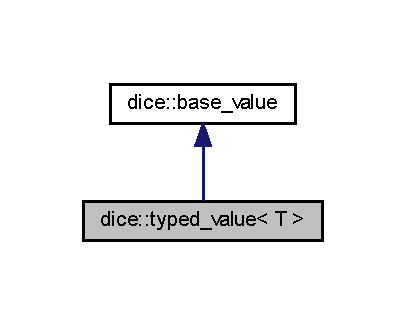
\includegraphics[width=195pt]{classdice_1_1typed__value__inherit__graph}
\end{center}
\end{figure}


Collaboration diagram for dice\+:\+:typed\+\_\+value$<$ T $>$\+:\nopagebreak
\begin{figure}[H]
\begin{center}
\leavevmode
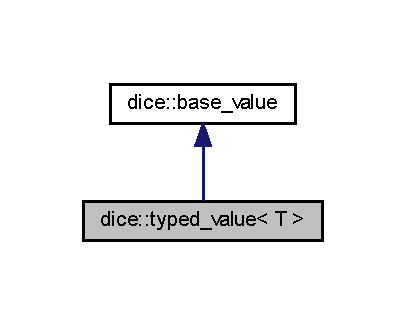
\includegraphics[width=195pt]{classdice_1_1typed__value__coll__graph}
\end{center}
\end{figure}
\subsection*{Public Types}
\begin{DoxyCompactItemize}
\item 
\mbox{\Hypertarget{classdice_1_1typed__value_a68dd4941f8e02bb9d4a7430530256887}\label{classdice_1_1typed__value_a68dd4941f8e02bb9d4a7430530256887}} 
using {\bfseries value\+\_\+type} = T
\end{DoxyCompactItemize}
\subsection*{Public Member Functions}
\begin{DoxyCompactItemize}
\item 
\mbox{\hyperlink{classdice_1_1typed__value_a44f8d5dc37013a90d605e67f71741837}{typed\+\_\+value}} (const value\+\_\+type \&value)
\begin{DoxyCompactList}\small\item\em Create value from data. \end{DoxyCompactList}\item 
\mbox{\hyperlink{classdice_1_1typed__value_a7cd2dad2087902ab85028fddf7c75c0b}{typed\+\_\+value}} (value\+\_\+type \&\&value)
\begin{DoxyCompactList}\small\item\em Create value from data. \end{DoxyCompactList}\item 
\mbox{\Hypertarget{classdice_1_1typed__value_a7ceb94854137f6ce6fbde9ce8d1b625a}\label{classdice_1_1typed__value_a7ceb94854137f6ce6fbde9ce8d1b625a}} 
{\bfseries typed\+\_\+value} (const \mbox{\hyperlink{classdice_1_1typed__value}{typed\+\_\+value}} \&)=delete
\item 
\mbox{\Hypertarget{classdice_1_1typed__value_a98cc3aaf7cfc64ec2cc5e64e66c8d9c0}\label{classdice_1_1typed__value_a98cc3aaf7cfc64ec2cc5e64e66c8d9c0}} 
void {\bfseries operator=} (const \mbox{\hyperlink{classdice_1_1typed__value}{typed\+\_\+value}} \&)=delete
\item 
\mbox{\Hypertarget{classdice_1_1typed__value_a3e8c1b40c238cf32e781a148baa03037}\label{classdice_1_1typed__value_a3e8c1b40c238cf32e781a148baa03037}} 
{\bfseries typed\+\_\+value} (\mbox{\hyperlink{classdice_1_1typed__value}{typed\+\_\+value}} \&\&)=default
\item 
\mbox{\Hypertarget{classdice_1_1typed__value_adfa842566fd143193eb0967a6b500626}\label{classdice_1_1typed__value_adfa842566fd143193eb0967a6b500626}} 
\mbox{\hyperlink{classdice_1_1typed__value}{typed\+\_\+value}} \& {\bfseries operator=} (\mbox{\hyperlink{classdice_1_1typed__value}{typed\+\_\+value}} \&\&)=default
\item 
\mbox{\hyperlink{value_8hpp_ab9af7d8ecc381e026ca4d07a745f23eb}{type\+\_\+id}} \mbox{\hyperlink{classdice_1_1typed__value_aa75a4167e6d3ff2640fd2fa65442e2ed}{type}} () const override
\begin{DoxyCompactList}\small\item\em Get type id of this type. \end{DoxyCompactList}\item 
void \mbox{\hyperlink{classdice_1_1typed__value_ae9563902b664c40a4b3d8a8cb201a194}{accept}} (\mbox{\hyperlink{classdice_1_1value__visitor}{value\+\_\+visitor}} $\ast$visitor) override
\begin{DoxyCompactList}\small\item\em Visit this value with given visitor. \end{DoxyCompactList}\item 
bool \mbox{\hyperlink{classdice_1_1typed__value_aeb5c87839a5e3ecb7beac6abc05e6701}{equals}} (const \mbox{\hyperlink{classdice_1_1base__value}{base\+\_\+value}} \&other) const override
\begin{DoxyCompactList}\small\item\em Compare 2 values. \end{DoxyCompactList}\item 
std\+::unique\+\_\+ptr$<$ \mbox{\hyperlink{classdice_1_1base__value}{base\+\_\+value}} $>$ \mbox{\hyperlink{classdice_1_1typed__value_a54490141b25b17213989fd2e859b4f59}{clone}} () const override
\begin{DoxyCompactList}\small\item\em Create a copy of this value. \end{DoxyCompactList}\item 
\mbox{\Hypertarget{classdice_1_1typed__value_a5033e424b0ff189d40ef51253f407ba0}\label{classdice_1_1typed__value_a5033e424b0ff189d40ef51253f407ba0}} 
value\+\_\+type \& {\bfseries data} ()
\item 
\mbox{\Hypertarget{classdice_1_1typed__value_addc189e4cc5c5be60cc5dd3911ae97f9}\label{classdice_1_1typed__value_addc189e4cc5c5be60cc5dd3911ae97f9}} 
const value\+\_\+type \& {\bfseries data} () const
\end{DoxyCompactItemize}
\subsection*{Static Public Member Functions}
\begin{DoxyCompactItemize}
\item 
\mbox{\Hypertarget{classdice_1_1typed__value_a8e3f3c7891feddcb9e0b7cb5727889eb}\label{classdice_1_1typed__value_a8e3f3c7891feddcb9e0b7cb5727889eb}} 
static \mbox{\hyperlink{value_8hpp_ab9af7d8ecc381e026ca4d07a745f23eb}{type\+\_\+id}} {\bfseries id} ()
\end{DoxyCompactItemize}


\subsection{Detailed Description}
\subsubsection*{template$<$typename T$>$\newline
class dice\+::typed\+\_\+value$<$ T $>$}

Value with data. 

\subsection{Constructor \& Destructor Documentation}
\mbox{\Hypertarget{classdice_1_1typed__value_a44f8d5dc37013a90d605e67f71741837}\label{classdice_1_1typed__value_a44f8d5dc37013a90d605e67f71741837}} 
\index{dice\+::typed\+\_\+value@{dice\+::typed\+\_\+value}!typed\+\_\+value@{typed\+\_\+value}}
\index{typed\+\_\+value@{typed\+\_\+value}!dice\+::typed\+\_\+value@{dice\+::typed\+\_\+value}}
\subsubsection{\texorpdfstring{typed\+\_\+value()}{typed\_value()}\hspace{0.1cm}{\footnotesize\ttfamily [1/2]}}
{\footnotesize\ttfamily template$<$typename T $>$ \\
\mbox{\hyperlink{classdice_1_1typed__value}{dice\+::typed\+\_\+value}}$<$ T $>$\+::\mbox{\hyperlink{classdice_1_1typed__value}{typed\+\_\+value}} (\begin{DoxyParamCaption}\item[{const value\+\_\+type \&}]{value }\end{DoxyParamCaption})\hspace{0.3cm}{\ttfamily [inline]}, {\ttfamily [explicit]}}



Create value from data. 


\begin{DoxyParams}{Parameters}
{\em value} & that will be copied \\
\hline
\end{DoxyParams}
\mbox{\Hypertarget{classdice_1_1typed__value_a7cd2dad2087902ab85028fddf7c75c0b}\label{classdice_1_1typed__value_a7cd2dad2087902ab85028fddf7c75c0b}} 
\index{dice\+::typed\+\_\+value@{dice\+::typed\+\_\+value}!typed\+\_\+value@{typed\+\_\+value}}
\index{typed\+\_\+value@{typed\+\_\+value}!dice\+::typed\+\_\+value@{dice\+::typed\+\_\+value}}
\subsubsection{\texorpdfstring{typed\+\_\+value()}{typed\_value()}\hspace{0.1cm}{\footnotesize\ttfamily [2/2]}}
{\footnotesize\ttfamily template$<$typename T $>$ \\
\mbox{\hyperlink{classdice_1_1typed__value}{dice\+::typed\+\_\+value}}$<$ T $>$\+::\mbox{\hyperlink{classdice_1_1typed__value}{typed\+\_\+value}} (\begin{DoxyParamCaption}\item[{value\+\_\+type \&\&}]{value }\end{DoxyParamCaption})\hspace{0.3cm}{\ttfamily [inline]}, {\ttfamily [explicit]}}



Create value from data. 


\begin{DoxyParams}{Parameters}
{\em value} & that will be moved \\
\hline
\end{DoxyParams}


\subsection{Member Function Documentation}
\mbox{\Hypertarget{classdice_1_1typed__value_ae9563902b664c40a4b3d8a8cb201a194}\label{classdice_1_1typed__value_ae9563902b664c40a4b3d8a8cb201a194}} 
\index{dice\+::typed\+\_\+value@{dice\+::typed\+\_\+value}!accept@{accept}}
\index{accept@{accept}!dice\+::typed\+\_\+value@{dice\+::typed\+\_\+value}}
\subsubsection{\texorpdfstring{accept()}{accept()}}
{\footnotesize\ttfamily template$<$typename T $>$ \\
void \mbox{\hyperlink{classdice_1_1typed__value}{dice\+::typed\+\_\+value}}$<$ T $>$\+::accept (\begin{DoxyParamCaption}\item[{\mbox{\hyperlink{classdice_1_1value__visitor}{value\+\_\+visitor}} $\ast$}]{visitor }\end{DoxyParamCaption})\hspace{0.3cm}{\ttfamily [inline]}, {\ttfamily [override]}, {\ttfamily [virtual]}}



Visit this value with given visitor. 


\begin{DoxyParams}{Parameters}
{\em visitor} & \\
\hline
\end{DoxyParams}


Implements \mbox{\hyperlink{classdice_1_1base__value_a8ab0acd9a7b10035a1c8f8a0f05b40b4}{dice\+::base\+\_\+value}}.

\mbox{\Hypertarget{classdice_1_1typed__value_a54490141b25b17213989fd2e859b4f59}\label{classdice_1_1typed__value_a54490141b25b17213989fd2e859b4f59}} 
\index{dice\+::typed\+\_\+value@{dice\+::typed\+\_\+value}!clone@{clone}}
\index{clone@{clone}!dice\+::typed\+\_\+value@{dice\+::typed\+\_\+value}}
\subsubsection{\texorpdfstring{clone()}{clone()}}
{\footnotesize\ttfamily template$<$typename T $>$ \\
std\+::unique\+\_\+ptr$<$\mbox{\hyperlink{classdice_1_1base__value}{base\+\_\+value}}$>$ \mbox{\hyperlink{classdice_1_1typed__value}{dice\+::typed\+\_\+value}}$<$ T $>$\+::clone (\begin{DoxyParamCaption}{ }\end{DoxyParamCaption}) const\hspace{0.3cm}{\ttfamily [inline]}, {\ttfamily [override]}, {\ttfamily [virtual]}}



Create a copy of this value. 

\begin{DoxyReturn}{Returns}
copied value 
\end{DoxyReturn}


Implements \mbox{\hyperlink{classdice_1_1base__value_a58335a522dda6d97332f938ead90aa15}{dice\+::base\+\_\+value}}.

\mbox{\Hypertarget{classdice_1_1typed__value_aeb5c87839a5e3ecb7beac6abc05e6701}\label{classdice_1_1typed__value_aeb5c87839a5e3ecb7beac6abc05e6701}} 
\index{dice\+::typed\+\_\+value@{dice\+::typed\+\_\+value}!equals@{equals}}
\index{equals@{equals}!dice\+::typed\+\_\+value@{dice\+::typed\+\_\+value}}
\subsubsection{\texorpdfstring{equals()}{equals()}}
{\footnotesize\ttfamily template$<$typename T $>$ \\
bool \mbox{\hyperlink{classdice_1_1typed__value}{dice\+::typed\+\_\+value}}$<$ T $>$\+::equals (\begin{DoxyParamCaption}\item[{const \mbox{\hyperlink{classdice_1_1base__value}{base\+\_\+value}} \&}]{other }\end{DoxyParamCaption}) const\hspace{0.3cm}{\ttfamily [inline]}, {\ttfamily [override]}, {\ttfamily [virtual]}}



Compare 2 values. 


\begin{DoxyParams}{Parameters}
{\em other} & value \\
\hline
\end{DoxyParams}
\begin{DoxyReturn}{Returns}
true iff both values have the same type and represent the same value (data() == other.\+data()) 
\end{DoxyReturn}


Implements \mbox{\hyperlink{classdice_1_1base__value_a81269be4c101eeef6d48810823e1835c}{dice\+::base\+\_\+value}}.

\mbox{\Hypertarget{classdice_1_1typed__value_aa75a4167e6d3ff2640fd2fa65442e2ed}\label{classdice_1_1typed__value_aa75a4167e6d3ff2640fd2fa65442e2ed}} 
\index{dice\+::typed\+\_\+value@{dice\+::typed\+\_\+value}!type@{type}}
\index{type@{type}!dice\+::typed\+\_\+value@{dice\+::typed\+\_\+value}}
\subsubsection{\texorpdfstring{type()}{type()}}
{\footnotesize\ttfamily template$<$typename T $>$ \\
\mbox{\hyperlink{value_8hpp_ab9af7d8ecc381e026ca4d07a745f23eb}{type\+\_\+id}} \mbox{\hyperlink{classdice_1_1typed__value}{dice\+::typed\+\_\+value}}$<$ T $>$\+::type (\begin{DoxyParamCaption}{ }\end{DoxyParamCaption}) const\hspace{0.3cm}{\ttfamily [inline]}, {\ttfamily [override]}, {\ttfamily [virtual]}}



Get type id of this type. 

\begin{DoxyReturn}{Returns}
type id of this type (\mbox{\hyperlink{value_8hpp_a7d7815802a2d6911ce76500f32b25399}{get\+\_\+type\+\_\+id$<$\+T$>$()}}) 
\end{DoxyReturn}


Implements \mbox{\hyperlink{classdice_1_1base__value_a5125d076b0ed6a398f4f4f8fe19ef60b}{dice\+::base\+\_\+value}}.



The documentation for this class was generated from the following file\+:\begin{DoxyCompactItemize}
\item 
C\+:/projects/dice/src/\mbox{\hyperlink{value_8hpp}{value.\+hpp}}\end{DoxyCompactItemize}

\hypertarget{classdice_1_1value__visitor}{}\section{dice\+:\+:value\+\_\+visitor Class Reference}
\label{classdice_1_1value__visitor}\index{dice\+::value\+\_\+visitor@{dice\+::value\+\_\+visitor}}


Visitor of a dice value.  




{\ttfamily \#include $<$value.\+hpp$>$}



Inheritance diagram for dice\+:\+:value\+\_\+visitor\+:\nopagebreak
\begin{figure}[H]
\begin{center}
\leavevmode
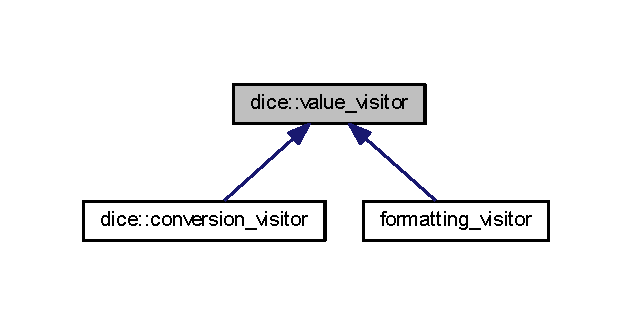
\includegraphics[width=304pt]{classdice_1_1value__visitor__inherit__graph}
\end{center}
\end{figure}
\subsection*{Public Member Functions}
\begin{DoxyCompactItemize}
\item 
\mbox{\Hypertarget{classdice_1_1value__visitor_a12a8d0f233ffced8b5c8f93327595e48}\label{classdice_1_1value__visitor_a12a8d0f233ffced8b5c8f93327595e48}} 
virtual void {\bfseries visit} (\mbox{\hyperlink{classdice_1_1typed__value}{typed\+\_\+value}}$<$ storage\+::int\+\_\+type $>$ $\ast$)=0
\item 
\mbox{\Hypertarget{classdice_1_1value__visitor_a5a140a4027d7bdb1a5f539afa2de59e2}\label{classdice_1_1value__visitor_a5a140a4027d7bdb1a5f539afa2de59e2}} 
virtual void {\bfseries visit} (\mbox{\hyperlink{classdice_1_1typed__value}{typed\+\_\+value}}$<$ storage\+::real\+\_\+type $>$ $\ast$)=0
\item 
\mbox{\Hypertarget{classdice_1_1value__visitor_a3ab1b89dacad2712686686047622ec1d}\label{classdice_1_1value__visitor_a3ab1b89dacad2712686686047622ec1d}} 
virtual void {\bfseries visit} (\mbox{\hyperlink{classdice_1_1typed__value}{typed\+\_\+value}}$<$ \mbox{\hyperlink{classdice_1_1decomposition}{storage\+::random\+\_\+variable\+\_\+type}} $>$ $\ast$)=0
\end{DoxyCompactItemize}


\subsection{Detailed Description}
Visitor of a dice value. 

The documentation for this class was generated from the following file\+:\begin{DoxyCompactItemize}
\item 
C\+:/projects/dice/src/\mbox{\hyperlink{value_8hpp}{value.\+hpp}}\end{DoxyCompactItemize}

\chapter{File Documentation}
\hypertarget{safe_8hpp}{}\section{C\+:/projects/dice/src/safe.hpp File Reference}
\label{safe_8hpp}\index{C\+:/projects/dice/src/safe.\+hpp@{C\+:/projects/dice/src/safe.\+hpp}}


Safe type for arithmetic operations on integral values.  


{\ttfamily \#include $<$limits$>$}\newline
{\ttfamily \#include $<$Safe\+Int3.\+hpp$>$}\newline
Include dependency graph for safe.\+hpp\+:\nopagebreak
\begin{figure}[H]
\begin{center}
\leavevmode
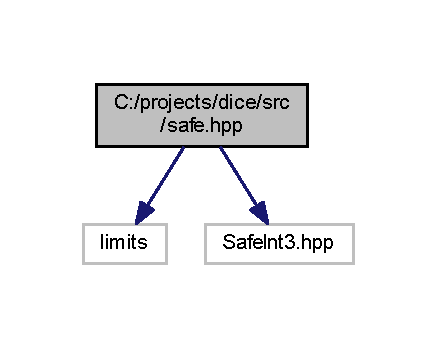
\includegraphics[width=210pt]{safe_8hpp__incl}
\end{center}
\end{figure}
This graph shows which files directly or indirectly include this file\+:\nopagebreak
\begin{figure}[H]
\begin{center}
\leavevmode
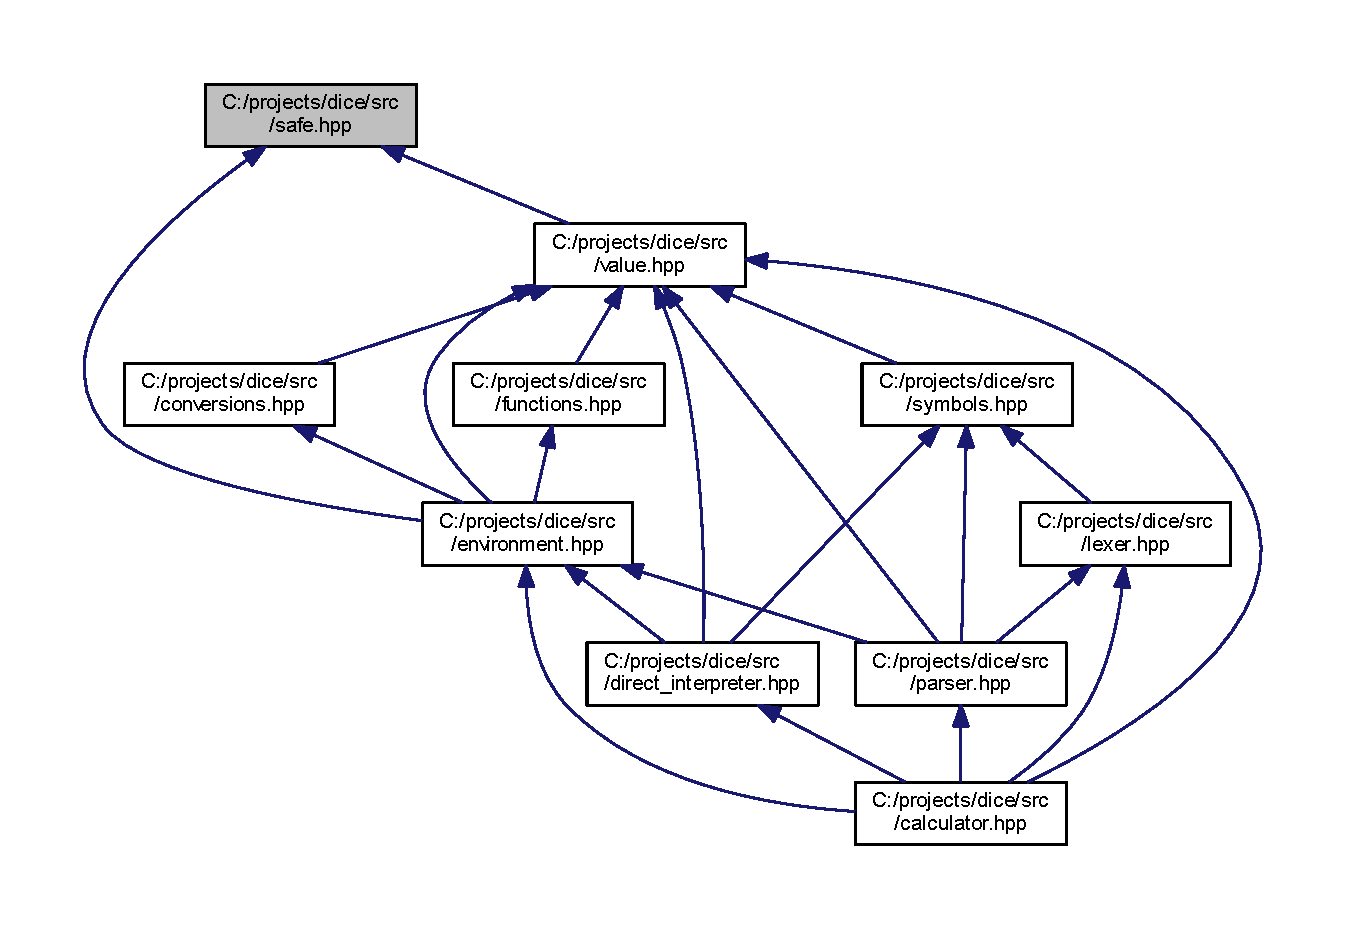
\includegraphics[width=350pt]{safe_8hpp__dep__incl}
\end{center}
\end{figure}
\subsection*{Classes}
\begin{DoxyCompactItemize}
\item 
struct \mbox{\hyperlink{structstd_1_1hash_3_01dice_1_1safe_3_01T_01_4_01_4}{std\+::hash$<$ dice\+::safe$<$ T $>$ $>$}}
\item 
class \mbox{\hyperlink{classstd_1_1numeric__limits_3_01dice_1_1safe_3_01T_01_4_01_4}{std\+::numeric\+\_\+limits$<$ dice\+::safe$<$ T $>$ $>$}}
\end{DoxyCompactItemize}
\subsection*{Macros}
\begin{DoxyCompactItemize}
\item 
\mbox{\Hypertarget{safe_8hpp_aa92d14d6f0ddfefa47082f5cf402caa2}\label{safe_8hpp_aa92d14d6f0ddfefa47082f5cf402caa2}} 
\#define {\bfseries N\+E\+E\+D\+S\+\_\+\+N\+U\+L\+L\+P\+T\+R\+\_\+\+D\+E\+F\+I\+N\+ED}~0
\end{DoxyCompactItemize}
\subsection*{Typedefs}
\begin{DoxyCompactItemize}
\item 
{\footnotesize template$<$typename T $>$ }\\using \mbox{\hyperlink{safe_8hpp_acd796e346e2b746739435c4a2983edba}{dice\+::safe}} = Safe\+Int$<$ T $>$
\begin{DoxyCompactList}\small\item\em Integral type with safe arithmetic operators. \end{DoxyCompactList}\item 
\mbox{\Hypertarget{safe_8hpp_a1f72ecd7606752bfe088742726caadcb}\label{safe_8hpp_a1f72ecd7606752bfe088742726caadcb}} 
using \mbox{\hyperlink{safe_8hpp_a1f72ecd7606752bfe088742726caadcb}{dice\+::safe\+\_\+int\+\_\+error}} = Safe\+Int\+Exception
\begin{DoxyCompactList}\small\item\em An error thrown when there is an overflow, underflow or divide by zero error. \end{DoxyCompactList}\end{DoxyCompactItemize}
\subsection*{Functions}
\begin{DoxyCompactItemize}
\item 
bool \mbox{\hyperlink{safe_8hpp_afd137ab6a0980246299511ba0f301858}{dice\+::is\+\_\+overflow\+\_\+error}} (const safe\+\_\+int\+\_\+error \&error)
\begin{DoxyCompactList}\small\item\em Check whether given exception is an overflow error. \end{DoxyCompactList}\item 
bool \mbox{\hyperlink{safe_8hpp_a9241d0fa80c1e5596015a540a4a21b7b}{dice\+::is\+\_\+divide\+\_\+by\+\_\+zero\+\_\+error}} (const safe\+\_\+int\+\_\+error \&error)
\begin{DoxyCompactList}\small\item\em Check whether given exception is an divide by zero error. \end{DoxyCompactList}\item 
\mbox{\Hypertarget{safe_8hpp_aeced5832cc1fd1b848df367fcbff680a}\label{safe_8hpp_aeced5832cc1fd1b848df367fcbff680a}} 
{\footnotesize template$<$typename T $>$ }\\\mbox{\hyperlink{safe_8hpp_acd796e346e2b746739435c4a2983edba}{dice\+::safe}}$<$ T $>$ {\bfseries std\+::max} (const \mbox{\hyperlink{safe_8hpp_acd796e346e2b746739435c4a2983edba}{dice\+::safe}}$<$ T $>$ \&a, const \mbox{\hyperlink{safe_8hpp_acd796e346e2b746739435c4a2983edba}{dice\+::safe}}$<$ T $>$ \&b)
\item 
\mbox{\Hypertarget{safe_8hpp_a5857b928dcee64cd9925906ae5366561}\label{safe_8hpp_a5857b928dcee64cd9925906ae5366561}} 
{\footnotesize template$<$typename T $>$ }\\\mbox{\hyperlink{safe_8hpp_acd796e346e2b746739435c4a2983edba}{dice\+::safe}}$<$ T $>$ {\bfseries std\+::max} (const \mbox{\hyperlink{safe_8hpp_acd796e346e2b746739435c4a2983edba}{dice\+::safe}}$<$ T $>$ \&a, const T \&b)
\item 
\mbox{\Hypertarget{safe_8hpp_a3be3da463310a7e462079dfd047d7d36}\label{safe_8hpp_a3be3da463310a7e462079dfd047d7d36}} 
{\footnotesize template$<$typename T $>$ }\\\mbox{\hyperlink{safe_8hpp_acd796e346e2b746739435c4a2983edba}{dice\+::safe}}$<$ T $>$ {\bfseries std\+::max} (const T \&a, const \mbox{\hyperlink{safe_8hpp_acd796e346e2b746739435c4a2983edba}{dice\+::safe}}$<$ T $>$ \&b)
\item 
\mbox{\Hypertarget{safe_8hpp_a25b47f00c0fa6cb4863c86de1fed10b5}\label{safe_8hpp_a25b47f00c0fa6cb4863c86de1fed10b5}} 
{\footnotesize template$<$typename T $>$ }\\\mbox{\hyperlink{safe_8hpp_acd796e346e2b746739435c4a2983edba}{dice\+::safe}}$<$ T $>$ {\bfseries std\+::min} (const \mbox{\hyperlink{safe_8hpp_acd796e346e2b746739435c4a2983edba}{dice\+::safe}}$<$ T $>$ \&a, const \mbox{\hyperlink{safe_8hpp_acd796e346e2b746739435c4a2983edba}{dice\+::safe}}$<$ T $>$ \&b)
\item 
\mbox{\Hypertarget{safe_8hpp_a38bf294087ffaf43b013bc084af3f316}\label{safe_8hpp_a38bf294087ffaf43b013bc084af3f316}} 
{\footnotesize template$<$typename T $>$ }\\\mbox{\hyperlink{safe_8hpp_acd796e346e2b746739435c4a2983edba}{dice\+::safe}}$<$ T $>$ {\bfseries std\+::min} (const \mbox{\hyperlink{safe_8hpp_acd796e346e2b746739435c4a2983edba}{dice\+::safe}}$<$ T $>$ \&a, const T \&b)
\item 
\mbox{\Hypertarget{safe_8hpp_a4deb6e583412717c3c3b9a6c56d3b9ed}\label{safe_8hpp_a4deb6e583412717c3c3b9a6c56d3b9ed}} 
{\footnotesize template$<$typename T $>$ }\\\mbox{\hyperlink{safe_8hpp_acd796e346e2b746739435c4a2983edba}{dice\+::safe}}$<$ T $>$ {\bfseries std\+::min} (const T \&a, const \mbox{\hyperlink{safe_8hpp_acd796e346e2b746739435c4a2983edba}{dice\+::safe}}$<$ T $>$ \&b)
\item 
\mbox{\Hypertarget{safe_8hpp_a79cfbd3d59a6e30c672c52a142f6f782}\label{safe_8hpp_a79cfbd3d59a6e30c672c52a142f6f782}} 
{\footnotesize template$<$typename T $>$ }\\void {\bfseries std\+::swap} (\mbox{\hyperlink{safe_8hpp_acd796e346e2b746739435c4a2983edba}{dice\+::safe}}$<$ T $>$ \&a, \mbox{\hyperlink{safe_8hpp_acd796e346e2b746739435c4a2983edba}{dice\+::safe}}$<$ T $>$ \&b)
\item 
\mbox{\Hypertarget{safe_8hpp_a671172f8a5b55c6bb968c10534553ce3}\label{safe_8hpp_a671172f8a5b55c6bb968c10534553ce3}} 
{\footnotesize template$<$typename T $>$ }\\std\+::ostream \& {\bfseries std\+::operator$<$$<$} (std\+::ostream \&output, \mbox{\hyperlink{safe_8hpp_acd796e346e2b746739435c4a2983edba}{dice\+::safe}}$<$ T $>$ \&value)
\item 
\mbox{\Hypertarget{safe_8hpp_ac5520589dbc09972ba26ea88eea56e95}\label{safe_8hpp_ac5520589dbc09972ba26ea88eea56e95}} 
{\footnotesize template$<$typename T $>$ }\\std\+::string {\bfseries std\+::to\+\_\+string} (const \mbox{\hyperlink{safe_8hpp_acd796e346e2b746739435c4a2983edba}{dice\+::safe}}$<$ T $>$ \&value)
\end{DoxyCompactItemize}


\subsection{Detailed Description}
Safe type for arithmetic operations on integral values. 



\subsection{Typedef Documentation}
\mbox{\Hypertarget{safe_8hpp_file_acd796e346e2b746739435c4a2983edba}\label{safe_8hpp_file_acd796e346e2b746739435c4a2983edba}} 
\index{safe.\+hpp@{safe.\+hpp}!safe@{safe}}
\index{safe@{safe}!safe.\+hpp@{safe.\+hpp}}
\subsubsection{\texorpdfstring{safe}{safe}}
{\footnotesize\ttfamily template$<$typename T $>$ \\
using \mbox{\hyperlink{safe_8hpp_acd796e346e2b746739435c4a2983edba}{dice\+::safe}} = typedef Safe\+Int$<$T$>$}



Integral type with safe arithmetic operators. 

For signed types, overflow, underflow and divide by zero all lead to an undefined behaviour. This type throws an exception (the safe\+\_\+int\+\_\+error type) in case of such error. 

\subsection{Function Documentation}
\mbox{\Hypertarget{safe_8hpp_file_a9241d0fa80c1e5596015a540a4a21b7b}\label{safe_8hpp_file_a9241d0fa80c1e5596015a540a4a21b7b}} 
\index{safe.\+hpp@{safe.\+hpp}!is\+\_\+divide\+\_\+by\+\_\+zero\+\_\+error@{is\+\_\+divide\+\_\+by\+\_\+zero\+\_\+error}}
\index{is\+\_\+divide\+\_\+by\+\_\+zero\+\_\+error@{is\+\_\+divide\+\_\+by\+\_\+zero\+\_\+error}!safe.\+hpp@{safe.\+hpp}}
\subsubsection{\texorpdfstring{is\+\_\+divide\+\_\+by\+\_\+zero\+\_\+error()}{is\_divide\_by\_zero\_error()}}
{\footnotesize\ttfamily bool dice\+::is\+\_\+divide\+\_\+by\+\_\+zero\+\_\+error (\begin{DoxyParamCaption}\item[{const \mbox{\hyperlink{safe_8hpp_a1f72ecd7606752bfe088742726caadcb}{safe\+\_\+int\+\_\+error}} \&}]{error }\end{DoxyParamCaption})\hspace{0.3cm}{\ttfamily [inline]}}



Check whether given exception is an divide by zero error. 


\begin{DoxyParams}{Parameters}
{\em error} & object\\
\hline
\end{DoxyParams}
\begin{DoxyReturn}{Returns}
true iff given exception is an divide by zero error 
\end{DoxyReturn}
\mbox{\Hypertarget{safe_8hpp_file_afd137ab6a0980246299511ba0f301858}\label{safe_8hpp_file_afd137ab6a0980246299511ba0f301858}} 
\index{safe.\+hpp@{safe.\+hpp}!is\+\_\+overflow\+\_\+error@{is\+\_\+overflow\+\_\+error}}
\index{is\+\_\+overflow\+\_\+error@{is\+\_\+overflow\+\_\+error}!safe.\+hpp@{safe.\+hpp}}
\subsubsection{\texorpdfstring{is\+\_\+overflow\+\_\+error()}{is\_overflow\_error()}}
{\footnotesize\ttfamily bool dice\+::is\+\_\+overflow\+\_\+error (\begin{DoxyParamCaption}\item[{const \mbox{\hyperlink{safe_8hpp_a1f72ecd7606752bfe088742726caadcb}{safe\+\_\+int\+\_\+error}} \&}]{error }\end{DoxyParamCaption})\hspace{0.3cm}{\ttfamily [inline]}}



Check whether given exception is an overflow error. 


\begin{DoxyParams}{Parameters}
{\em error} & object\\
\hline
\end{DoxyParams}
\begin{DoxyReturn}{Returns}
true iff given exception is an overflow error 
\end{DoxyReturn}

\hypertarget{symbols_8hpp}{}\section{C\+:/projects/dice/src/symbols.hpp File Reference}
\label{symbols_8hpp}\index{C\+:/projects/dice/src/symbols.\+hpp@{C\+:/projects/dice/src/symbols.\+hpp}}


Symbols in dice expressions (returned by lexer).  


{\ttfamily \#include $<$string$>$}\newline
{\ttfamily \#include $<$memory$>$}\newline
{\ttfamily \#include $<$type\+\_\+traits$>$}\newline
{\ttfamily \#include \char`\"{}value.\+hpp\char`\"{}}\newline
Include dependency graph for symbols.\+hpp\+:\nopagebreak
\begin{figure}[H]
\begin{center}
\leavevmode
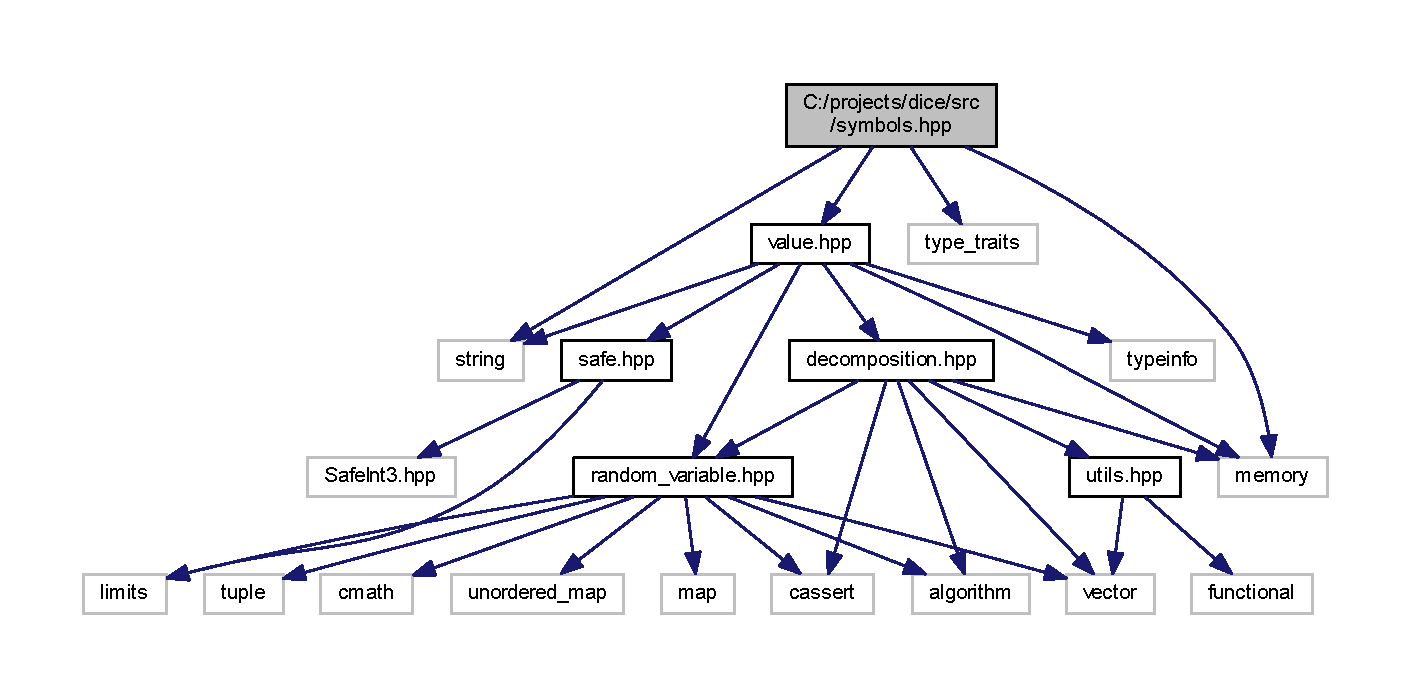
\includegraphics[width=350pt]{symbols_8hpp__incl}
\end{center}
\end{figure}
This graph shows which files directly or indirectly include this file\+:\nopagebreak
\begin{figure}[H]
\begin{center}
\leavevmode
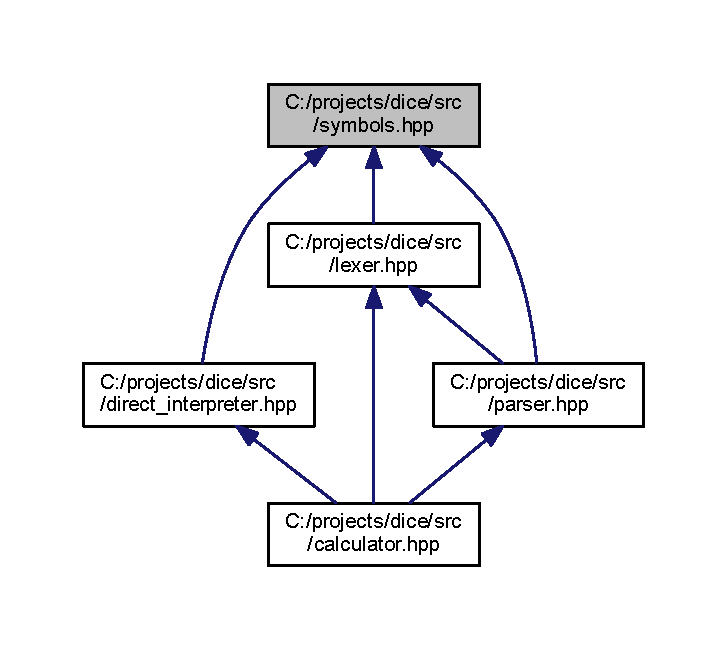
\includegraphics[width=349pt]{symbols_8hpp__dep__incl}
\end{center}
\end{figure}
\subsection*{Classes}
\begin{DoxyCompactItemize}
\item 
struct \mbox{\hyperlink{structdice_1_1symbol}{dice\+::symbol}}
\begin{DoxyCompactList}\small\item\em Terminal symbol returned by the lexer type. \end{DoxyCompactList}\end{DoxyCompactItemize}
\subsection*{Enumerations}
\begin{DoxyCompactItemize}
\item 
enum \mbox{\hyperlink{symbols_8hpp_ab0295a855bb7eadc138abd6993af3aea}{dice\+::symbol\+\_\+type}} \{ \newline
{\bfseries plus}, 
{\bfseries minus}, 
{\bfseries times}, 
{\bfseries divide}, 
\newline
{\bfseries rel\+\_\+op}, 
{\bfseries roll\+\_\+op}, 
{\bfseries in}, 
{\bfseries left\+\_\+paren}, 
\newline
{\bfseries right\+\_\+paren}, 
{\bfseries left\+\_\+square\+\_\+bracket}, 
{\bfseries right\+\_\+square\+\_\+bracket}, 
{\bfseries param\+\_\+delim}, 
\newline
{\bfseries semicolon}, 
{\bfseries var}, 
{\bfseries assign}, 
{\bfseries number}, 
\newline
{\bfseries func\+\_\+id}, 
{\bfseries id}, 
{\bfseries end}
 \}
\begin{DoxyCompactList}\small\item\em Type of a terminal symbol. \end{DoxyCompactList}\end{DoxyCompactItemize}
\subsection*{Functions}
\begin{DoxyCompactItemize}
\item 
std\+::string \mbox{\hyperlink{symbols_8hpp_aa542a90d900a186cee459f53537bc037}{dice\+::to\+\_\+string}} (const symbol \&symbol)
\begin{DoxyCompactList}\small\item\em Convert given symbol to string. \end{DoxyCompactList}\item 
std\+::string \mbox{\hyperlink{symbols_8hpp_a92dc762419e41c64e4c25bf2e44e4fa2}{dice\+::to\+\_\+string}} (symbol\+\_\+type type)
\begin{DoxyCompactList}\small\item\em Convert given symbol type to string. \end{DoxyCompactList}\end{DoxyCompactItemize}


\subsection{Detailed Description}
Symbols in dice expressions (returned by lexer). 



\subsection{Enumeration Type Documentation}
\mbox{\Hypertarget{symbols_8hpp_file_ab0295a855bb7eadc138abd6993af3aea}\label{symbols_8hpp_file_ab0295a855bb7eadc138abd6993af3aea}} 
\index{symbols.\+hpp@{symbols.\+hpp}!symbol\+\_\+type@{symbol\+\_\+type}}
\index{symbol\+\_\+type@{symbol\+\_\+type}!symbols.\+hpp@{symbols.\+hpp}}
\subsubsection{\texorpdfstring{symbol\+\_\+type}{symbol\_type}}
{\footnotesize\ttfamily enum \mbox{\hyperlink{symbols_8hpp_ab0295a855bb7eadc138abd6993af3aea}{dice\+::symbol\+\_\+type}}\hspace{0.3cm}{\ttfamily [strong]}}



Type of a terminal symbol. 



\subsection{Function Documentation}
\mbox{\Hypertarget{symbols_8hpp_file_aa542a90d900a186cee459f53537bc037}\label{symbols_8hpp_file_aa542a90d900a186cee459f53537bc037}} 
\index{symbols.\+hpp@{symbols.\+hpp}!to\+\_\+string@{to\+\_\+string}}
\index{to\+\_\+string@{to\+\_\+string}!symbols.\+hpp@{symbols.\+hpp}}
\subsubsection{\texorpdfstring{to\+\_\+string()}{to\_string()}\hspace{0.1cm}{\footnotesize\ttfamily [1/2]}}
{\footnotesize\ttfamily std\+::string dice\+::to\+\_\+string (\begin{DoxyParamCaption}\item[{const \mbox{\hyperlink{structdice_1_1symbol}{symbol}} \&}]{symbol }\end{DoxyParamCaption})}



Convert given symbol to string. 


\begin{DoxyParams}{Parameters}
{\em symbol} & \\
\hline
\end{DoxyParams}
\begin{DoxyReturn}{Returns}
string representation of the symbol for debugging and error messages. 
\end{DoxyReturn}
\mbox{\Hypertarget{symbols_8hpp_file_a92dc762419e41c64e4c25bf2e44e4fa2}\label{symbols_8hpp_file_a92dc762419e41c64e4c25bf2e44e4fa2}} 
\index{symbols.\+hpp@{symbols.\+hpp}!to\+\_\+string@{to\+\_\+string}}
\index{to\+\_\+string@{to\+\_\+string}!symbols.\+hpp@{symbols.\+hpp}}
\subsubsection{\texorpdfstring{to\+\_\+string()}{to\_string()}\hspace{0.1cm}{\footnotesize\ttfamily [2/2]}}
{\footnotesize\ttfamily std\+::string dice\+::to\+\_\+string (\begin{DoxyParamCaption}\item[{\mbox{\hyperlink{symbols_8hpp_ab0295a855bb7eadc138abd6993af3aea}{symbol\+\_\+type}}}]{type }\end{DoxyParamCaption})}



Convert given symbol type to string. 


\begin{DoxyParams}{Parameters}
{\em type} & of a symbol\\
\hline
\end{DoxyParams}
\begin{DoxyReturn}{Returns}
string representation of the symbol type for debugging and error messages. 
\end{DoxyReturn}

\hypertarget{utils_8hpp}{}\section{C\+:/projects/dice/src/utils.hpp File Reference}
\label{utils_8hpp}\index{C\+:/projects/dice/src/utils.\+hpp@{C\+:/projects/dice/src/utils.\+hpp}}


General purpose utility function templates.  


{\ttfamily \#include $<$vector$>$}\newline
{\ttfamily \#include $<$functional$>$}\newline
Include dependency graph for utils.\+hpp\+:\nopagebreak
\begin{figure}[H]
\begin{center}
\leavevmode
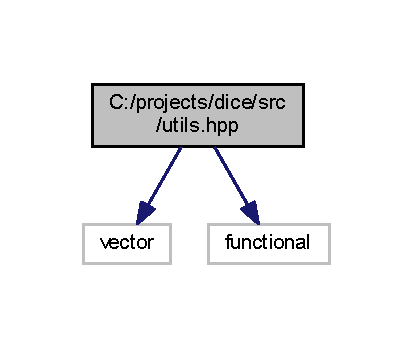
\includegraphics[width=198pt]{utils_8hpp__incl}
\end{center}
\end{figure}
This graph shows which files directly or indirectly include this file\+:\nopagebreak
\begin{figure}[H]
\begin{center}
\leavevmode
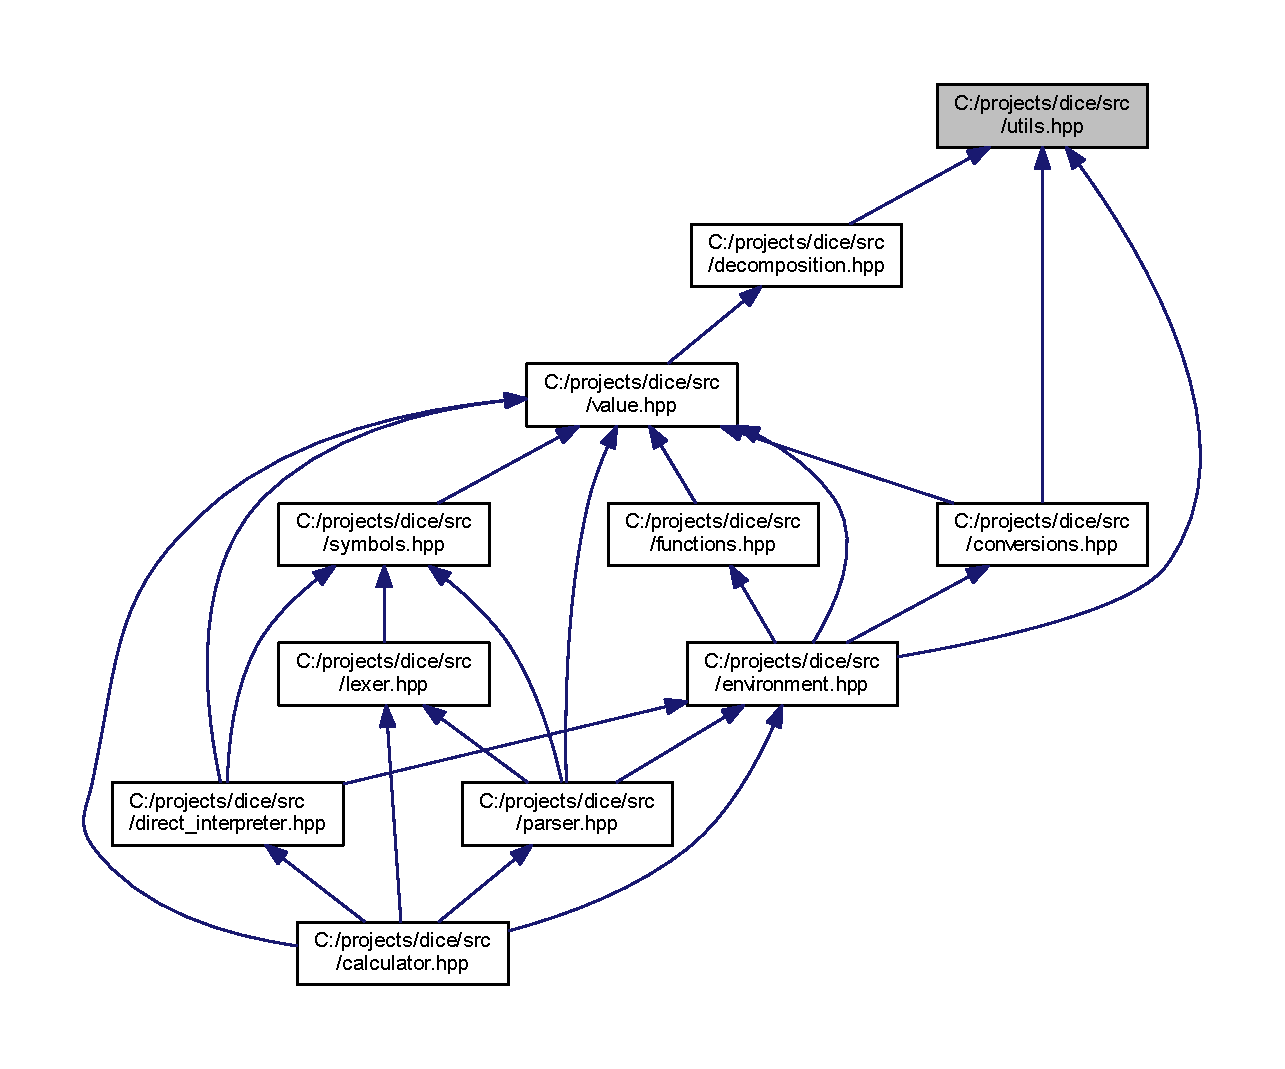
\includegraphics[width=350pt]{utils_8hpp__dep__incl}
\end{center}
\end{figure}
\subsection*{Functions}
\begin{DoxyCompactItemize}
\item 
{\footnotesize template$<$typename T , typename Less  = std\+::less$<$\+T$>$$>$ }\\std\+::vector$<$ T $>$ \mbox{\hyperlink{utils_8hpp_a76c303cd6d428781aba0af2068485c7e}{dice\+::sorted\+\_\+union}} (const std\+::vector$<$ T $>$ \&a, const std\+::vector$<$ T $>$ \&b, Less is\+\_\+less=Less())
\begin{DoxyCompactList}\small\item\em Compute union of sorted lists A and B. \end{DoxyCompactList}\item 
{\footnotesize template$<$typename T $>$ }\\T \mbox{\hyperlink{utils_8hpp_ab5f71aca381e999396a566ef7ef794e1}{dice\+::clamp}} (const T \&value, const T \&lower, const T \&upper)
\begin{DoxyCompactList}\small\item\em Clamp a value to given range. \end{DoxyCompactList}\end{DoxyCompactItemize}


\subsection{Detailed Description}
General purpose utility function templates. 



\subsection{Function Documentation}
\mbox{\Hypertarget{utils_8hpp_file_ab5f71aca381e999396a566ef7ef794e1}\label{utils_8hpp_file_ab5f71aca381e999396a566ef7ef794e1}} 
\index{utils.\+hpp@{utils.\+hpp}!clamp@{clamp}}
\index{clamp@{clamp}!utils.\+hpp@{utils.\+hpp}}
\subsubsection{\texorpdfstring{clamp()}{clamp()}}
{\footnotesize\ttfamily template$<$typename T $>$ \\
T dice\+::clamp (\begin{DoxyParamCaption}\item[{const T \&}]{value,  }\item[{const T \&}]{lower,  }\item[{const T \&}]{upper }\end{DoxyParamCaption})}



Clamp a value to given range. 


\begin{DoxyParams}{Parameters}
{\em value} & \\
\hline
{\em lower} & bound of the range \\
\hline
{\em upper} & bound of the range\\
\hline
\end{DoxyParams}
\begin{DoxyReturn}{Returns}
lower if value $<$ lower upper if value $>$ upper value otherwise 
\end{DoxyReturn}
\mbox{\Hypertarget{utils_8hpp_file_a76c303cd6d428781aba0af2068485c7e}\label{utils_8hpp_file_a76c303cd6d428781aba0af2068485c7e}} 
\index{utils.\+hpp@{utils.\+hpp}!sorted\+\_\+union@{sorted\+\_\+union}}
\index{sorted\+\_\+union@{sorted\+\_\+union}!utils.\+hpp@{utils.\+hpp}}
\subsubsection{\texorpdfstring{sorted\+\_\+union()}{sorted\_union()}}
{\footnotesize\ttfamily template$<$typename T , typename Less  = std\+::less$<$\+T$>$$>$ \\
std\+::vector$<$T$>$ dice\+::sorted\+\_\+union (\begin{DoxyParamCaption}\item[{const std\+::vector$<$ T $>$ \&}]{a,  }\item[{const std\+::vector$<$ T $>$ \&}]{b,  }\item[{Less}]{is\+\_\+less = {\ttfamily Less()} }\end{DoxyParamCaption})}



Compute union of sorted lists A and B. 

Both lists have to be sorted by given comparer.


\begin{DoxyParams}{Parameters}
{\em a} & sorted list A \\
\hline
{\em b} & sorted list B \\
\hline
{\em is\+\_\+less} & comparer (use operator $<$ by default)\\
\hline
\end{DoxyParams}
\begin{DoxyReturn}{Returns}
sorted union of lists A and B 
\end{DoxyReturn}

\hypertarget{value_8hpp}{}\section{C\+:/projects/dice/src/value.hpp File Reference}
\label{value_8hpp}\index{C\+:/projects/dice/src/value.\+hpp@{C\+:/projects/dice/src/value.\+hpp}}


Value in a dice expression.  


{\ttfamily \#include $<$memory$>$}\newline
{\ttfamily \#include $<$string$>$}\newline
{\ttfamily \#include $<$typeinfo$>$}\newline
{\ttfamily \#include \char`\"{}safe.\+hpp\char`\"{}}\newline
{\ttfamily \#include \char`\"{}random\+\_\+variable.\+hpp\char`\"{}}\newline
{\ttfamily \#include \char`\"{}decomposition.\+hpp\char`\"{}}\newline
Include dependency graph for value.\+hpp\+:\nopagebreak
\begin{figure}[H]
\begin{center}
\leavevmode
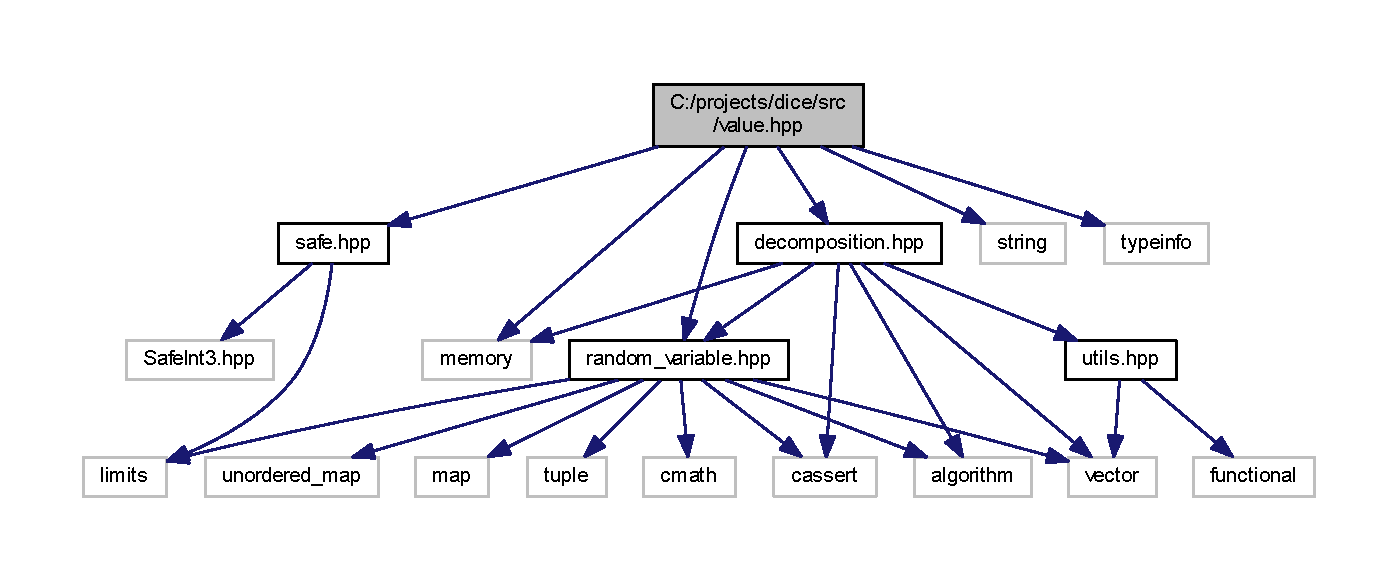
\includegraphics[width=350pt]{value_8hpp__incl}
\end{center}
\end{figure}
This graph shows which files directly or indirectly include this file\+:\nopagebreak
\begin{figure}[H]
\begin{center}
\leavevmode
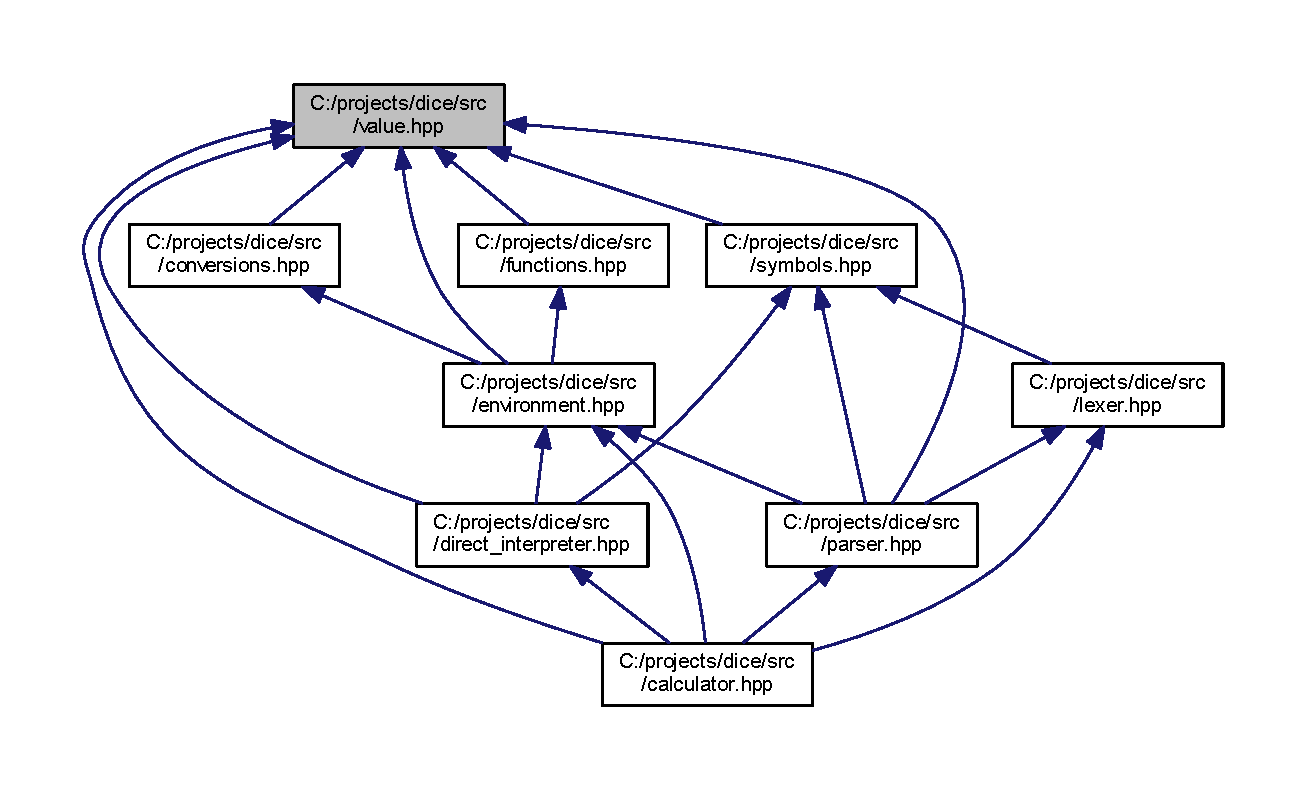
\includegraphics[width=350pt]{value_8hpp__dep__incl}
\end{center}
\end{figure}
\subsection*{Classes}
\begin{DoxyCompactItemize}
\item 
class \mbox{\hyperlink{classdice_1_1typed__value}{dice\+::typed\+\_\+value$<$ T $>$}}
\begin{DoxyCompactList}\small\item\em Value with data. \end{DoxyCompactList}\item 
class \mbox{\hyperlink{classdice_1_1value__visitor}{dice\+::value\+\_\+visitor}}
\begin{DoxyCompactList}\small\item\em Visitor of a dice value. \end{DoxyCompactList}\item 
class \mbox{\hyperlink{classdice_1_1base__value}{dice\+::base\+\_\+value}}
\begin{DoxyCompactList}\small\item\em Parent of all value types that are used in dice expressions. \end{DoxyCompactList}\item 
class \mbox{\hyperlink{classdice_1_1typed__value}{dice\+::typed\+\_\+value$<$ T $>$}}
\begin{DoxyCompactList}\small\item\em Value with data. \end{DoxyCompactList}\end{DoxyCompactItemize}
\subsection*{Typedefs}
\begin{DoxyCompactItemize}
\item 
\mbox{\Hypertarget{value_8hpp_a0cee38bdc43f4a004e131e53eb579917}\label{value_8hpp_a0cee38bdc43f4a004e131e53eb579917}} 
using {\bfseries dice\+::storage\+::int\+\_\+type} = safe$<$ int $>$
\item 
\mbox{\Hypertarget{value_8hpp_a84b40525b369ed2862ee37ffc78673e2}\label{value_8hpp_a84b40525b369ed2862ee37ffc78673e2}} 
using {\bfseries dice\+::storage\+::real\+\_\+type} = double
\item 
\mbox{\Hypertarget{value_8hpp_a95475a7e7b6b0e8f0ac5738de5dbe59e}\label{value_8hpp_a95475a7e7b6b0e8f0ac5738de5dbe59e}} 
using {\bfseries dice\+::storage\+::random\+\_\+variable\+\_\+type} = decomposition$<$ int\+\_\+type, real\+\_\+type $>$
\item 
\mbox{\Hypertarget{value_8hpp_ae08dd7aa0330f19098bf0f1037736ffe}\label{value_8hpp_ae08dd7aa0330f19098bf0f1037736ffe}} 
using {\bfseries dice\+::type\+\_\+int} = typed\+\_\+value$<$ storage\+::int\+\_\+type $>$
\item 
\mbox{\Hypertarget{value_8hpp_a03a6944f1b609de16641192c30896552}\label{value_8hpp_a03a6944f1b609de16641192c30896552}} 
using {\bfseries dice\+::type\+\_\+real} = typed\+\_\+value$<$ storage\+::real\+\_\+type $>$
\item 
\mbox{\Hypertarget{value_8hpp_ac1a2b326ac4f73f62389ba9c351f4da5}\label{value_8hpp_ac1a2b326ac4f73f62389ba9c351f4da5}} 
using {\bfseries dice\+::type\+\_\+rand\+\_\+var} = typed\+\_\+value$<$ storage\+::random\+\_\+variable\+\_\+type $>$
\end{DoxyCompactItemize}
\subsection*{Enumerations}
\begin{DoxyCompactItemize}
\item 
\mbox{\Hypertarget{value_8hpp_ab9af7d8ecc381e026ca4d07a745f23eb}\label{value_8hpp_ab9af7d8ecc381e026ca4d07a745f23eb}} 
enum \mbox{\hyperlink{value_8hpp_ab9af7d8ecc381e026ca4d07a745f23eb}{dice\+::type\+\_\+id}} \{ {\bfseries integer}, 
{\bfseries real}, 
{\bfseries random\+\_\+variable}
 \}
\begin{DoxyCompactList}\small\item\em Type identifier of a value in a dice expression. \end{DoxyCompactList}\end{DoxyCompactItemize}
\subsection*{Functions}
\begin{DoxyCompactItemize}
\item 
\mbox{\Hypertarget{value_8hpp_a7d7815802a2d6911ce76500f32b25399}\label{value_8hpp_a7d7815802a2d6911ce76500f32b25399}} 
{\footnotesize template$<$typename Value\+Type $>$ }\\type\+\_\+id \mbox{\hyperlink{value_8hpp_a7d7815802a2d6911ce76500f32b25399}{dice\+::get\+\_\+type\+\_\+id}} ()
\begin{DoxyCompactList}\small\item\em Translate C++ types to type\+\_\+id. \end{DoxyCompactList}\item 
\mbox{\Hypertarget{value_8hpp_afbaba9142b81828196eea597f31b2ccc}\label{value_8hpp_afbaba9142b81828196eea597f31b2ccc}} 
{\footnotesize template$<$$>$ }\\type\+\_\+id {\bfseries dice\+::get\+\_\+type\+\_\+id$<$ storage\+::int\+\_\+type $>$} ()
\item 
\mbox{\Hypertarget{value_8hpp_a578498bd6f298412ad6372e04b15711e}\label{value_8hpp_a578498bd6f298412ad6372e04b15711e}} 
{\footnotesize template$<$$>$ }\\type\+\_\+id {\bfseries dice\+::get\+\_\+type\+\_\+id$<$ storage\+::real\+\_\+type $>$} ()
\item 
\mbox{\Hypertarget{value_8hpp_a13f9d948fef2b5fb98782562194d8f81}\label{value_8hpp_a13f9d948fef2b5fb98782562194d8f81}} 
{\footnotesize template$<$$>$ }\\type\+\_\+id {\bfseries dice\+::get\+\_\+type\+\_\+id$<$ storage\+::random\+\_\+variable\+\_\+type $>$} ()
\item 
std\+::string \mbox{\hyperlink{value_8hpp_af848a0ca9b1baba1d52fe6fbbe28e9b2}{dice\+::to\+\_\+string}} (type\+\_\+id tid)
\begin{DoxyCompactList}\small\item\em Convert type id to a human readable string. \end{DoxyCompactList}\item 
{\footnotesize template$<$typename T , typename... Value$>$ }\\std\+::unique\+\_\+ptr$<$ T $>$ \mbox{\hyperlink{value_8hpp_a6c2eca285fa025fbf228f56ccad8f8e8}{dice\+::make}} (Value \&\&... data)
\begin{DoxyCompactList}\small\item\em Create a value used in dice expressions. \end{DoxyCompactList}\end{DoxyCompactItemize}


\subsection{Detailed Description}
Value in a dice expression. 



\subsection{Function Documentation}
\mbox{\Hypertarget{value_8hpp_file_a6c2eca285fa025fbf228f56ccad8f8e8}\label{value_8hpp_file_a6c2eca285fa025fbf228f56ccad8f8e8}} 
\index{value.\+hpp@{value.\+hpp}!make@{make}}
\index{make@{make}!value.\+hpp@{value.\+hpp}}
\subsubsection{\texorpdfstring{make()}{make()}}
{\footnotesize\ttfamily template$<$typename T , typename... Value$>$ \\
std\+::unique\+\_\+ptr$<$T$>$ dice\+::make (\begin{DoxyParamCaption}\item[{Value \&\&...}]{data }\end{DoxyParamCaption})}



Create a value used in dice expressions. 


\begin{DoxyTemplParams}{Template Parameters}
{\em T} & type of the value. It has to be derived from base\+\_\+value. T\+::value\+\_\+type has to be defined and the type T has to have a constructor with T\+::value\+\_\+type as its argumnet. \\
\hline
{\em Value} & types of argumnets passed to the construction of T\+::value\+\_\+type.\\
\hline
\end{DoxyTemplParams}

\begin{DoxyParams}{Parameters}
{\em data} & argumnets forwarded to the constructor of T\+::value\+\_\+type.\\
\hline
\end{DoxyParams}
\begin{DoxyReturn}{Returns}
new value (pointer to base\+\_\+value) 
\end{DoxyReturn}
\mbox{\Hypertarget{value_8hpp_file_af848a0ca9b1baba1d52fe6fbbe28e9b2}\label{value_8hpp_file_af848a0ca9b1baba1d52fe6fbbe28e9b2}} 
\index{value.\+hpp@{value.\+hpp}!to\+\_\+string@{to\+\_\+string}}
\index{to\+\_\+string@{to\+\_\+string}!value.\+hpp@{value.\+hpp}}
\subsubsection{\texorpdfstring{to\+\_\+string()}{to\_string()}}
{\footnotesize\ttfamily std\+::string dice\+::to\+\_\+string (\begin{DoxyParamCaption}\item[{\mbox{\hyperlink{value_8hpp_ab9af7d8ecc381e026ca4d07a745f23eb}{type\+\_\+id}}}]{tid }\end{DoxyParamCaption})\hspace{0.3cm}{\ttfamily [inline]}}



Convert type id to a human readable string. 


\begin{DoxyParams}{Parameters}
{\em tid} & id of a type\\
\hline
\end{DoxyParams}
\begin{DoxyReturn}{Returns}
name of the type 
\end{DoxyReturn}

%--- End generated contents ---

% Index
\backmatter
\newpage
\phantomsection
\clearemptydoublepage
\addcontentsline{toc}{chapter}{Index}
\printindex

\end{document}
